%\documentclass[final,3p,times,twocolumn]{elsarticle}
\documentclass[authoryear,preprint,review,11pt,doubleblind]{elsarticle}
%\documentclass[authoryear,preprint,review,11pt]{elsarticle}


    %% Use the option review to obtain double line spacing
    %% \documentclass[authoryear,preprint,review,12pt]{elsarticle}

    %% Use the options 1p,twocolumn; 3p; 3p,twocolumn; 5p; or 5p,twocolumn
    %% for a journal layout:
    %% \documentclass[final,1p,times]{elsarticle}
    %% \documentclass[final,1p,times,twocolumn]{elsarticle}
    %% \documentclass[final,3p,times]{elsarticle}
    %% \documentclass[final,3p,times,twocolumn]{elsarticle}
    %% \documentclass[final,5p,times]{elsarticle}
    %% \documentclass[final,5p,times,twocolumn]{elsarticle}
\usepackage[utf8x]{inputenc}
    \usepackage{amssymb}
    \usepackage{svg}
    \usepackage{lineno}
    \usepackage[colorlinks=true,linkcolor=blue]{hyperref}%
    \usepackage{orcidlink}
    \usepackage{setspace}
    \usepackage{tabularx}
    \usepackage{xltabular}
    \usepackage{longtable}
    \usepackage{ltablex}
    \usepackage{booktabs}
    \usepackage{multirow}
    \usepackage{hyperref}
    \usepackage{dirtytalk}
    \usepackage[english]{babel}
    \usepackage{pdflscape}
    \usepackage{float}
 \usepackage{caption}
\usepackage{subcaption}

  
    %\usepackage{csquotes}
    \usepackage{microtype}
    \interfootnotelinepenalty=10000
    %\onehalfspacing %TODO Remove Line before final export
    %Path relative to the main .tex file 
    \graphicspath{ {./Figures/} }

    \journal{Sustainable Cities and Society}
    \begin{document}
    \newcolumntype{L}{>{\raggedleft\arraybackslash}X}
    \begin{frontmatter}

    %% Title, authors and addresses

    %% use the tnoteref command within \title for footnotes;
    %% use the tnotetext command for the associated footnote;
    %% use the fnref command within \author or \address for footnotes;
    %% use the fntext command for the associated footnote;
    %% use the corref command within \author for corresponding author footnotes;
    %% use the cortext command for the associated footnote;
    %% use the ead command for the email address,
    %% and the form \ead[url] for the home page:
    %% \title{Title\tnoteref{label1}}
    %% \tnotetext[label1]{}
    %% \author{Name\corref{cor1}\fnref{label2}}
    %% \ead{email address}
    %% \ead[url]{home page}
    %% \fntext[label2]{}
    %% \cortext[cor1]{}
    %% \affiliation{organization={},
    %%             addressline={},
    %%             city={},
    %%             postcode={},
    %%             state={},
    %%             country={}}
    %% \fntext[label3]{}

    \title{URBAN DIGITAL TWIN-BASED SOLUTION USING  GEOSPATIAL INFORMATION FOR SOLID WASTE MANAGEMENT}

    \author[Utwente]{Iván Cárdenas-León\corref{cor1}\,\orcidlink{0009-0005-0245-633X}}
    \affiliation[Utwente]{organization={Faculty of Geo-Information Science and Earth Observation (ITC), University of Twente},%Department and Organization
                addressline={Hallenweg 8}, 
                city={Enschede},
                postcode={7522 NH}, 
                state={Overijssel},
                country={Netherlands}}

    \cortext[cor1]{Corresponding author}
    \ead{i.l.cardenasleon@utwente.nl}
    %\credit{Conceptualization, Data curation, Investigation, Formal Analysis, Visualization, Methodology, Software, Writing - original draft}

    \author[Utwente]{Mila Koeva\,\orcidlink{0000-0001-7612-5270}}
    %\credit{Supervision, Project administration, Writing - review \& editing}
    \author[Utwente]{Pirouz Nourian\,\orcidlink{0000-0002-3817-7931}}
    %\credit{Supervision, Writing - review \& editing}
    \author[UPretoria]{Calayde Davey\,\orcidlink{0000-0001-9249-5829}}
    %\credit{Conceptualization, Data curation, Supervision \& editing}

    \affiliation[UPretoria]{organization={Department of Architecture, Faculty of Engineering, Built Environment and Information Technology, University of Pretoria},%Department and Organization
                addressline={Private Bag x 20}, 
                city={Hatfield},
                postcode={0028}, 
                state={Gauteng},
                country={South Africa}}

    \begin{abstract}
    \label{sec:abstract}
    With over 2 billion metric tons generated annually, global solid waste (SW) production has severe environmental consequences. Though not a primary SDG, effective waste management (SWM) is vital for meeting targets 11.6, 12.4, and 12.5. South Africa, in particular, deals with significant SW generation and inadequate collection services. Therefore, this paper presents a Urban Digital Twin (UDT) protoptype to tackle these issues, involving stakeholder prioritization, integrating real-time monitoring, citizen participation, waste generation simulations, optimized collection routes, and a control Dashboard where stakeholders' system requirements were included. With the UDT, optimized collection routes are proposed that reduces fuel use, operational costs, and emissions. The opinions of the stakeholders on the usefulness of the UDT varied due to their backgrounds and skills. Most of them appreciated the Dashboard visualization and the UDT possibilities for resource optimization. The performance of the UDT depends on computer capacity and local or online processing. This UDT prototype sets the foundation for digital twinning in SWM, scalable to different areas, vehicles, and production levels. Our Digital twinning approach, citizen involvement, and multi-stakeholder engagement enhance the SWM, particularly benefiting resource-limited countries.
    \end{abstract}

    %TODO: Get Graphical abstract and Highlights
    % %%Graphical abstract
    % % \begin{graphicalabstract}
    % %     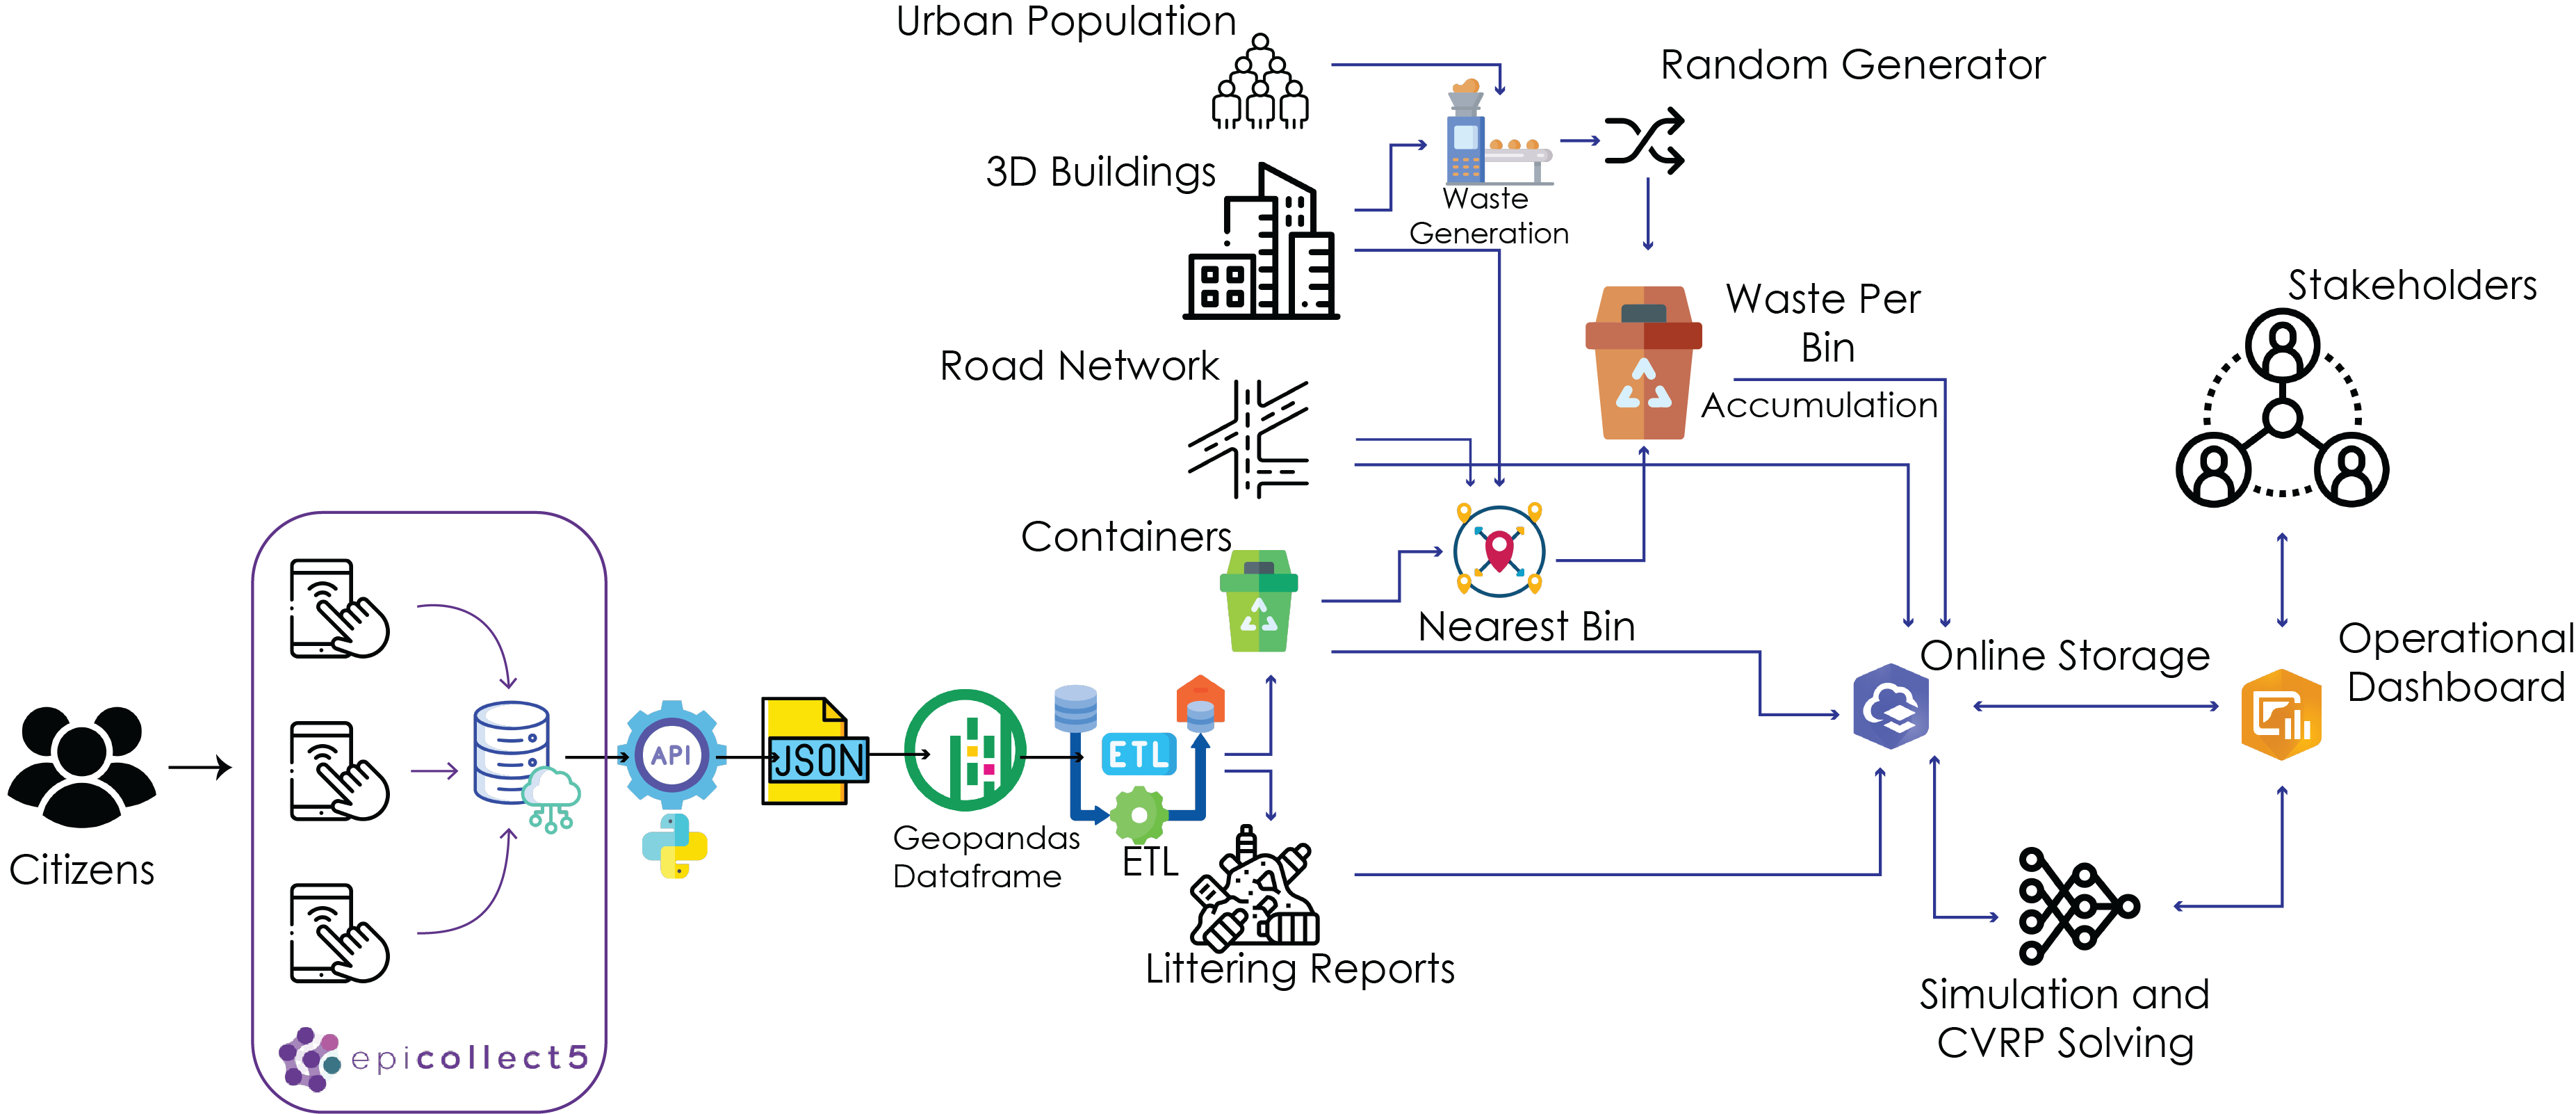
\includegraphics[width=\textwidth]{Figures/System Architecture.png}
    % % \end{graphicalabstract}

    % % % %%Research highlights
    % % \begin{highlights}
    % %\todo[inline]{add Highlights}
    % \item Solid Waste Digital Twin architecture for improved waste management.
    % \item Stakeholder engagement for fit-to-context design.
    % \item Integration of Geo-information for solid waste daily generation estimation.
    % \item Network analysis for saturated containers waste collection.
    % \item Interactive dashboard for operational control of solid waste collection.
    % \end{highlights}

    \begin{keyword}
    
    %% keywords here, in the form: keyword \sep keyword
    Digital Twins \sep Solid Waste Management \sep Citizen Science \sep Volunteered Geographical Information (VGI) \sep Vehicle Routing Problem (VRP)
    \end{keyword}   
    \end{frontmatter}

    %\linenumbers
    %% main text

    \section{Introduction}
    \label{sec:Intro}
    Urban Digital Twin (UDT) refers to a digital replica of some of the physical assets of a district or neighborhood of a city that can be used to co-create and test scenarios with city-specific parameters \citep{Ruohomaki2018}. It goes beyond the static 2D or 3D representation, becoming a model for the past, present, and future state \citep{geohubDigitalTwinningUrban2022}. %Digital twinning aims to provide mechanisms for understanding the spatial dynamics and the impacts of climate change, biodiversity loss, permeability, unsustainable transport, and effects of anthropogenic impacts on the city environment \citep{caprariDigitalTwin22}. 
    A UDT %falls within the Augmented Urban Planning framework for strategic planning \citep{Azadi2023}
    and can work as a Decision Support System to inform urban planners and designers of the impact a project development will have and be a driver for citizen involvement in the planning process \citep{Dembski2019, Dembski2020}. Although there has been some advancements in interesting UDTs into  well-known urban challenges such as air quality \citep{Mak2021}, traffic management \citep{Ibrahim2022}, parking occupancy, or parking restrictions \citep{latreCityThingsIntegrated2016}, some other city challenges have been left behind, such as underground management, water supply or urban greenery.

    %UDTs have a process of \textit{data feeding - information response - implementation reaction} cycle that can move in near-real time and operate as urban computing workflows through web communication and processing \citep{Nourian2018}. Most cities use Internet of Things (IoT) devices to feed initial data into the UDT development cycle\citep{abadiaSystematicSurveyInternet2022}.% Using sensors that communicate through technologies such as Wi-Fi, mobile networks (3G/4G/5G), 6LoWAN, Bluetooth, Radio or NFC \citep{Balaji2019},  

    Solid waste (SW) management is another one of these challenges. It has been identified as an important topic for integrating such sensors to improve urban sustainability, as it significantly impacts the quality of urban life \citep{Ismagilova2019}. According to the World Bank, around 2.24 billion metric tons of municipal SW was generated in 2020 worldwide \citep{Kaza2021}.% This number increased as medical waste during the COVID-19 pandemic contributed to these values, ranging between 62\% and 350\%, according to  \citep{Yousefi2021}, or between 18\% and 425\%, according to \citep{Liang2021}.
    Of the overall annual waste generation, around 33\% is not being managed in environmentally safe ways \citep{Kaza2018}. 

    The United Nations does not include SW management as a primary Sustainable Development Goal (SDG), potentially reducing its visibility in the political agenda \citep{rodicResolvingGovernanceIssues2017}. However, tackling the issue is intrinsically related to twelve of the 17 SDGs, principally SDGs 11, 12, and 13 \citep{Wilson2015}. Therefore, waste management is critical for achieving holistic sustainability in cities.
    
%Many UDTs in the global north often begin with a top-down IoT-first approach. However, in other world regions (such as the global south), advanced communications infrastructure and institutional knowledge are not mature enough to start UDTs from that position. To activate local UDT initiatives in such regions may need an alternative, bottom-up, and people-first approach instead.

    Previous studies have incorporated the use of geospatial data, such as land use, road network configuration, street slope \citep{Hina2020, Sahib2021, Malakahmad2014} and computer vision for identifying containers  \citep{Moral2022} in the improvement of SW collection. However, there has not been an integrated approach that includes a 3D estimation of waste generation, citizen-tagged container location, and route collection improvement.

    %As such, this paper aims to advance sustainable waste management practices holistically, improve urban cleanliness, reduce environmental impacts, and enhance the overall quality of life in rapidly growing developing world urban areas. 
    As such, This study presents a UDT prototype that incorporates waste generation simulations of containers and vehicle routing optimization based on the generation and prediction of future waste volumes. The study area is the Hatfield and Hillcrest neighborhoods in the City of Tshwane (CoT), South Africa. This research presents the first South African Digital Twin model for SW management based on volunteered geographical information, 3D LiDAR city scans, 3D waste generation calculations, and open-source geospatial data. This proposes a UDT waste prototype that might be replicated in other regions.

This paper is a continuation of the work originally presented in The 18th 3DGeoInfo conference \citep{cardenasivanSolidWasteVirtual24}. Here, we explore integrating urban digital twin technology with solid waste management systems to address the challenges of waste collection, intermittence, and illegal dumping in urban environments.

    \subsection{Background}
    \label{subsec:Background}
    \subsubsection{Geogrpahical context}
In South Africa, 30.5 million tons of residential, commercial and institutional solid waste were generated in 2017 \cite
    
    In the City of Tshwane, the administrative capital of South Africa, protests have arisen due to irregularities in urban service provision. Residents are advocating for equitable service delivery and consistency equivalent to that of the historically privileged white areas of the city during apartheid \citep{Mokebe2018}. Following a major municipal services strike in 2023, the CoT has since restored its waste removal schedule after grappling with many challenges from the illegal strike affecting service delivery \citep{berlintonCityEmployees23}. While city officials note general improvements in waste operations across all seven city regions, illegal dumping remains a significant concern, posing health risks. Residents are encouraged to report uncollected bins regularly, and residents from all walks of society play an important role in maintaining the city's cleanliness \citep{ramadieCityTshwane23, njiloTshwaneBattles23}. 
   
   The city reports that the SW that reaches the landfill per capita is around 1.95kg/d \citep{tshwaneCityTshwane20222022}, indicating waste production is higher than the national average. With over six hundred illegal dumping hotspots detected, the city has identified measures to improve the SW management system, including confirming illegal dumping sites, allocating new containers, and applying intense cleanup of streets \citep{tshwaneConsolidatedAuditedAnnual2022}. Previous studies suggest that executing the type of measures, such as the ones identified by CoT, requires moving from a traditional static model to a dynamic one that adapts to changes in waste generation, incorporates real-time container monitoring and frequent collection route optimization \citep{Anagnostopoulos2015b, Hina2020, Ramson2022}. Moreover, the model should include active citizen participation supported by government structures for improved SW management \citep{kubanzaSustainableSolidWaste2020}.
   
    \subsubsection{Solid waste monitoring}
    \label{subsubsec:Monitoring}
    SW container identification has been done via survey \citep{alsobkySmartFramework23}, on-field road-by-road data collection \citep{ kiranCharacterizationQuantification23} or data directly sourced from local authorities \citep{Hina2020}. Advanced approaches propose video recordings where cameras are integrated into collection vehicles and post-processed through computer vision techniques to geo-locate and classify container types in a city \citep{Moral2022}. These approaches help to identify \textit{where} SW should be collected but do not monitor \textit{fullness} (capacity or current saturation state).
    
    Several monitoring sensors for solid waste saturation or container \textit{fullness} have been designed. Some include ultrasonic sensors on container lids \citep{Chaudhari2018, Joshi2022, Karthik2021, Mahajan2017, Ramson2017}, weight sensors at the bottom of containers \citep{Rovetta2009}, mixes of both \citep{Ali2020, Vicentini2009} or infrared sensors \citep{Singh2016}. The cited studies using ultrasonic sensors were only tested at the prototype level, limited to two containers, and data is later reported to a centralized system. These sensors still need to be tested in outdoor conditions of cities and scaled to several containers to test realistic management and operations scenarios. Nonetheless, \citet{Ali2020} simulations demonstrated the possibility of creating production records and using these to forecast daily generation levels for individual containers.

    While Rovetta et al. and Vicentini et al. tested ultrasonic sensors outdoors in Shanghai (PR China) with controlled scenarios for residential and commercial usage, these tests used human operators for reporting containers. Citizens were invited to use particular containers, creating a bias in the actual values of on-site volume generation. These studies also propose including route optimization for waste collection in conjunction with the sensors. However, they do not implement this with real-time information.

   Utrecht, Netherlands, has already incorporated ultrasound sensors and daily rerouting based on \textit{fullness} of containers. This approach reduces the required vehicles and prevents container overflow \citep{utrechtUndergroundContainersMunicipality2021}, demonstrating the systemic value of integrating the sensors with route optimization.

\subsubsection{Routing optimization based on geospatial information}
    \label{subsubsec:routing}
    SW collection is an inverse goods distribution problem - items must be collected instead of delivered. Necessarily, any waste collection route optimizations improve the efficiencies of waste collection systems. Collection route optimization problems depend on the number of collection points, waiting times for loading and unloading, accumulated distances between landfills and collection points, and distances between collection points \citep{Sarmah2019}.

 Route optimization is a well-studied topic and has many different approaches. Analytical approaches focus on mathematical methods that analyze efficiency for improving collection routes. For example, research that focuses on changes in road-length segments shows reductions in cost, energy, or vehicle operating times, while vehicles using less fuel also allow an increase of area coverage \citep{erdincRouteOptimizationElectric2019, Hannan2018, Sahib2021}. Agent-based modeling approaches can simulate SW generation and sequential filling of collected containers based on the shortest routes between filled containers, which helps maximize potential profits \citep{Likotiko2017}. Geospatial information approaches show how network analysis could be implemented using route lengths, topography, and collection times \citep{Hemidat2017, Jovicic2010, Malakahmad2014}. Approaches can be integrated, for example, where mathematical route optimizing use of road networks, traffic data, and geospatial collection scheme information are combined and tested against agent-based model simulations \citep{nguyen-trongOptimizationMunicipalSolid2017}. These vehicle routing optimization problems all share typical constraints: 1) clear start- and end-points for each route (depot or landfill), 2) each container is served by only one route, 3) vehicle collection capacity limits, and 4)  comply with local traffic regulations.

    The approaches show reductions in operation times, fuel savings, and human work hours. Only \citet{Likotiko2017} considers consecutive optimizations based on container volumes or \textit{fullness} and waste production dynamics, such as constant changes in SW generation, which would require real-time data that can re-optimize routes. However, these optimization approaches aim to produce one-fit-for-all solutions rather than adapt to unique area requirements and local waste generation dynamics.

    \subsubsection{Stakeholder identification and classification}
    \label{subsubsec:stakeholders}
    Waste management systems include dynamic and interrelated technological, political, environmental, and socio-economic aspects, including diverse stakeholders \citep{Zaman2011}. Understanding stakeholder characteristics, concerns, local conditions, and constraints helps increase participation, effectiveness, and willingness to find appropriate solutions \citep{Lishan2021, palacios-agundezIntegratingStakeholdersDemands2014}. Defining the UDT use case for complex, interrelated issues (such as urban waste management) requires balancing stakeholder interests. Therefore, it is important to understand the stakeholder landscape, context, relationships, and the particularities of what is at stake \citep{Freeman2010}.

     Stakeholder salience theory \citep{Mitchell1997, Shafique2022} classifies stakeholders on three attributes: \textit{Power}, \textit{Urgency},  \textit{Legitimacy}, and \textit{Proximity}. This stakeholder framework has 16 typologies classification that helps to distinguish between  stakeholders, delineating their roles and limitations according to the possession, or exclusion, of each attributes. According to this classification, Definitive and crucial stakeholders take the most important roles in project operation and management (See Figure \ref{fig:figure2})
    
    % %\begin{figure}[htb]
    %     \centering
    %     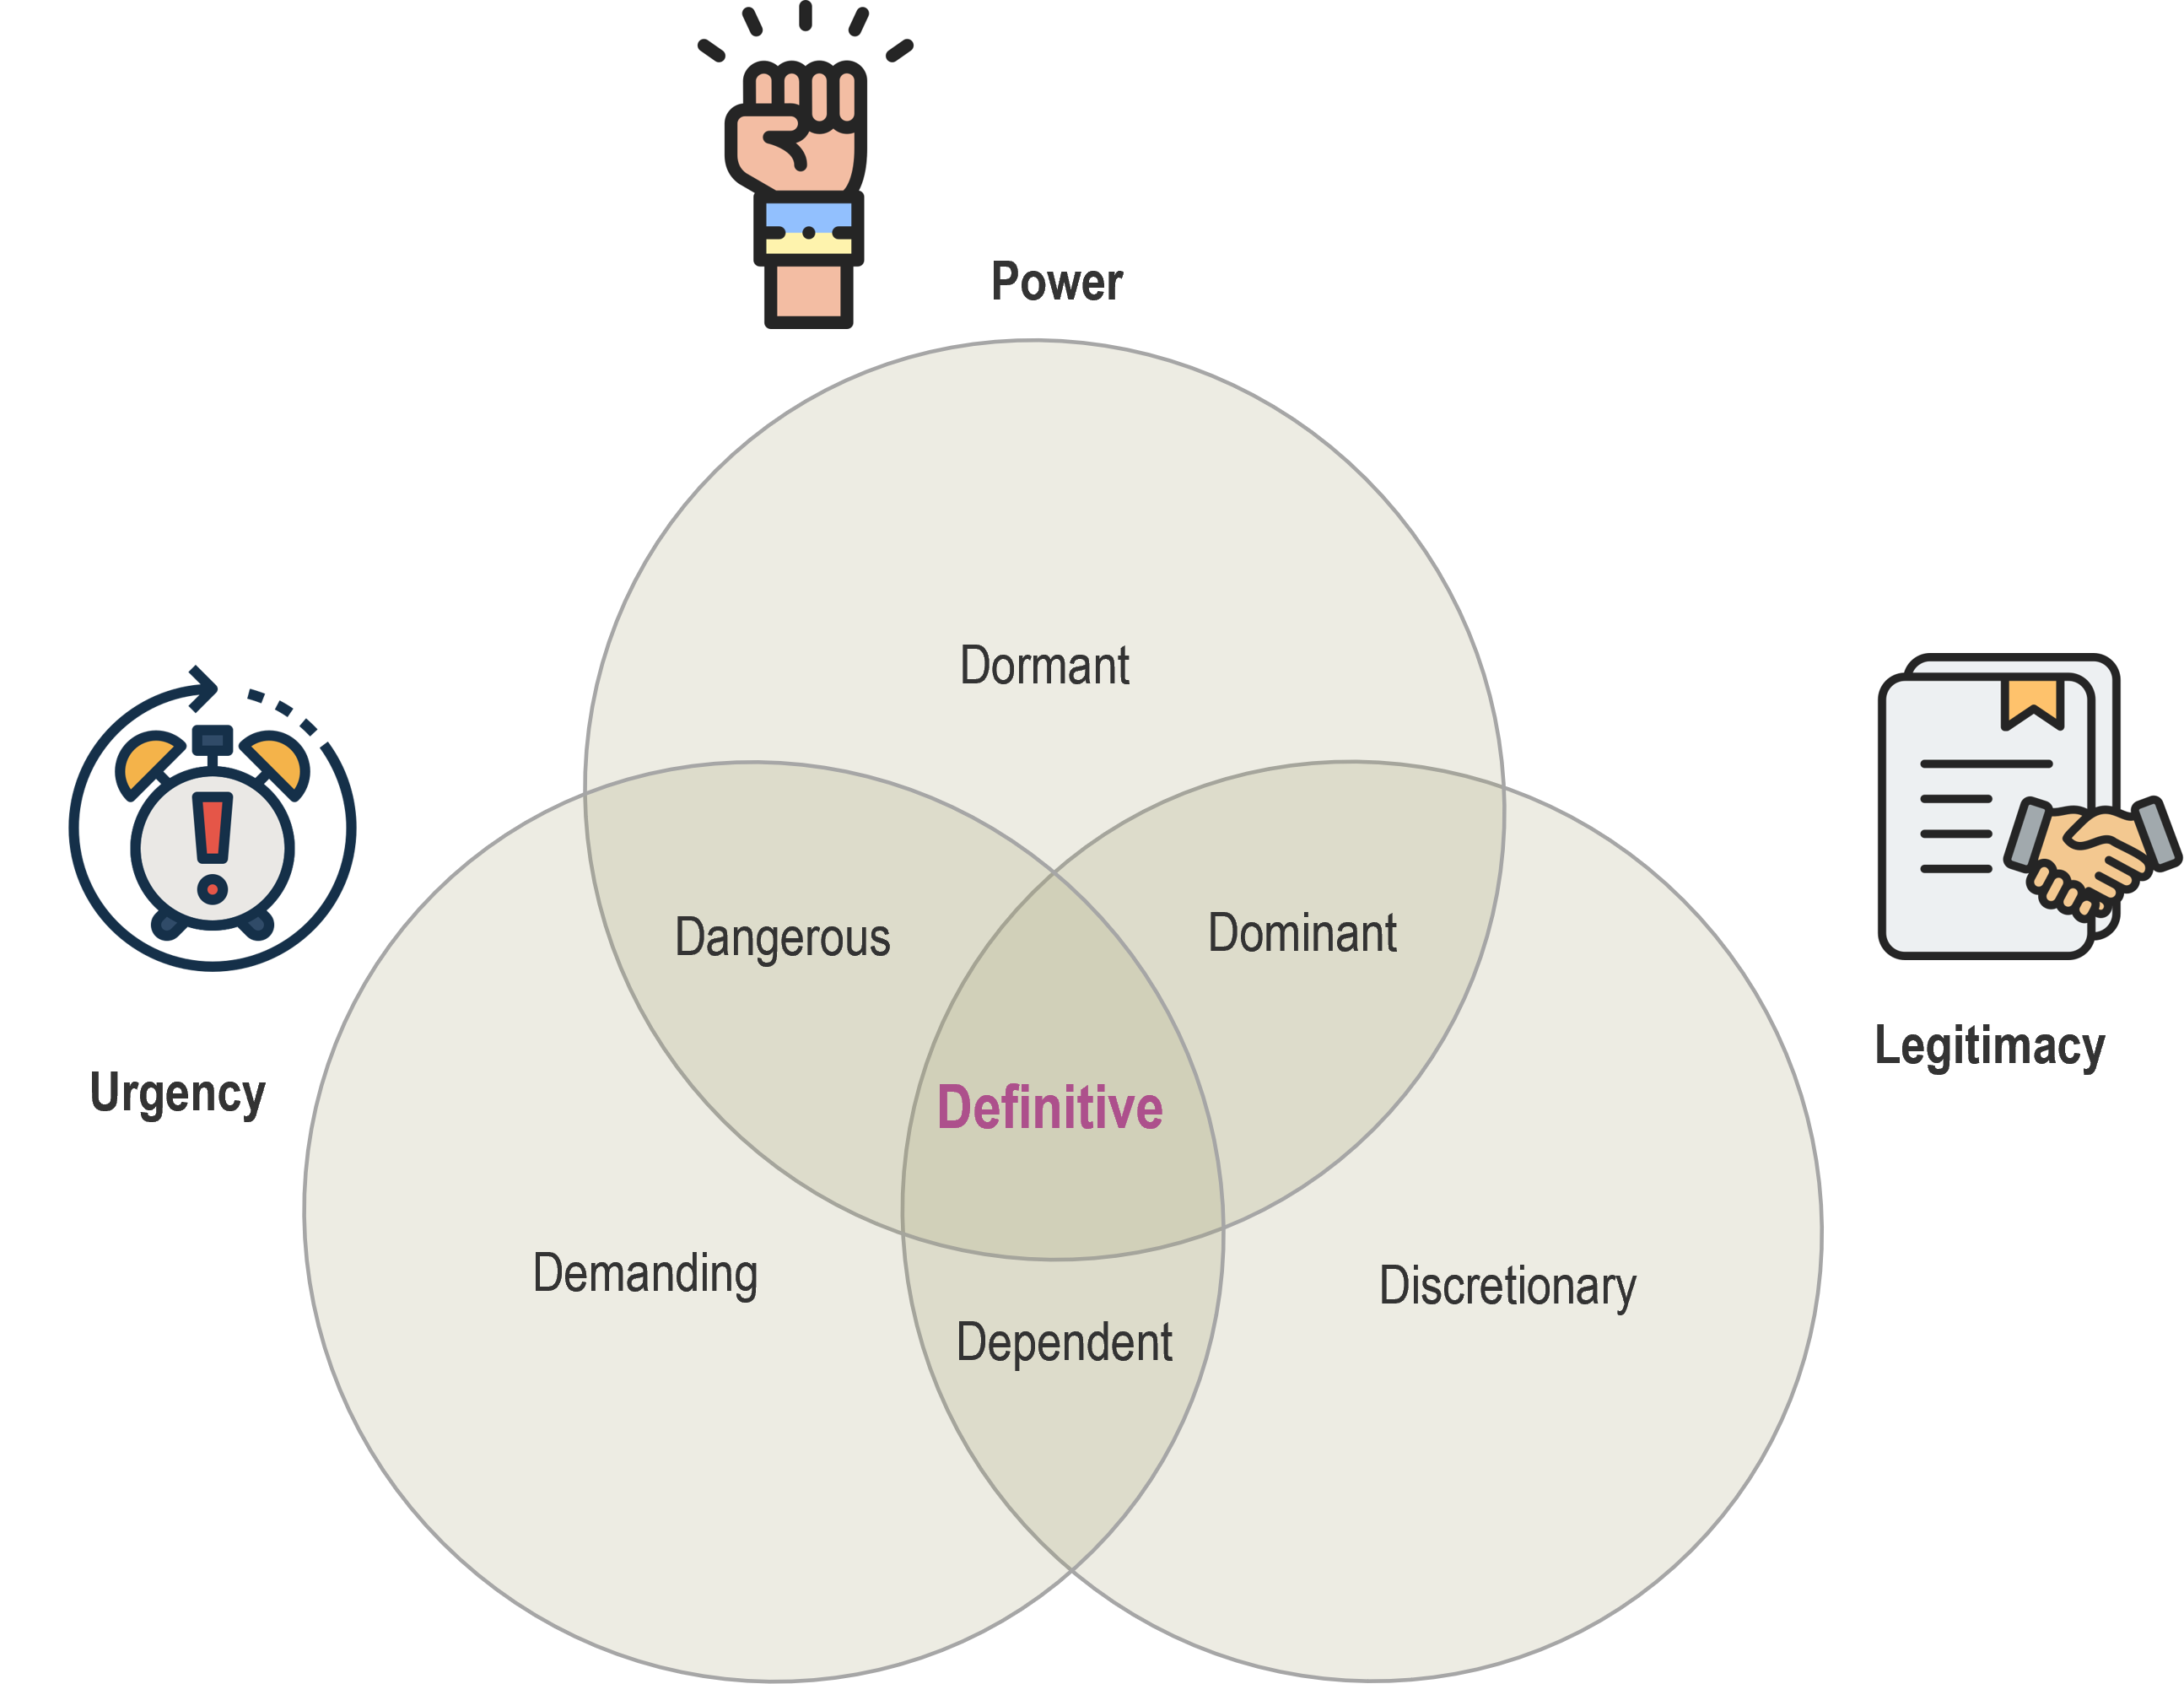
\includegraphics[width=0.8\columnwidth]{Stakeholders Mitchel.png}
    %     \caption{Stakeholders Typology. One, two, or three attributes are present. Source: Mitchel et al. (1997)}
    %     \label{fig:graph1}
    % \end{figure}

    % Critics of Mitchell, et al.'s model argue that it overlooks vulnerable stakeholders, especially those who lack in the main attributes \citep{Shafique2022}. \citet{Driscoll2004} suggests incorporating spatial and temporal dimensions, emphasizing the importance of physical and social proximity influencing stakeholder relationships. \citet{Shafique2022} closes the spatial-temporal gap by introducing \textit{Proximity} as an independent attribute, coexisting with \textit{Power}, \textit{Urgency}, and \textit{Legitimacy} (Figure \ref{fig:figure2}) Their adapted salient model expands to eight stakeholder classifications including vulnerable stakeholders and aspects of project operations beyond organizational management.
    
    \begin{figure}[!h]
        \centering
        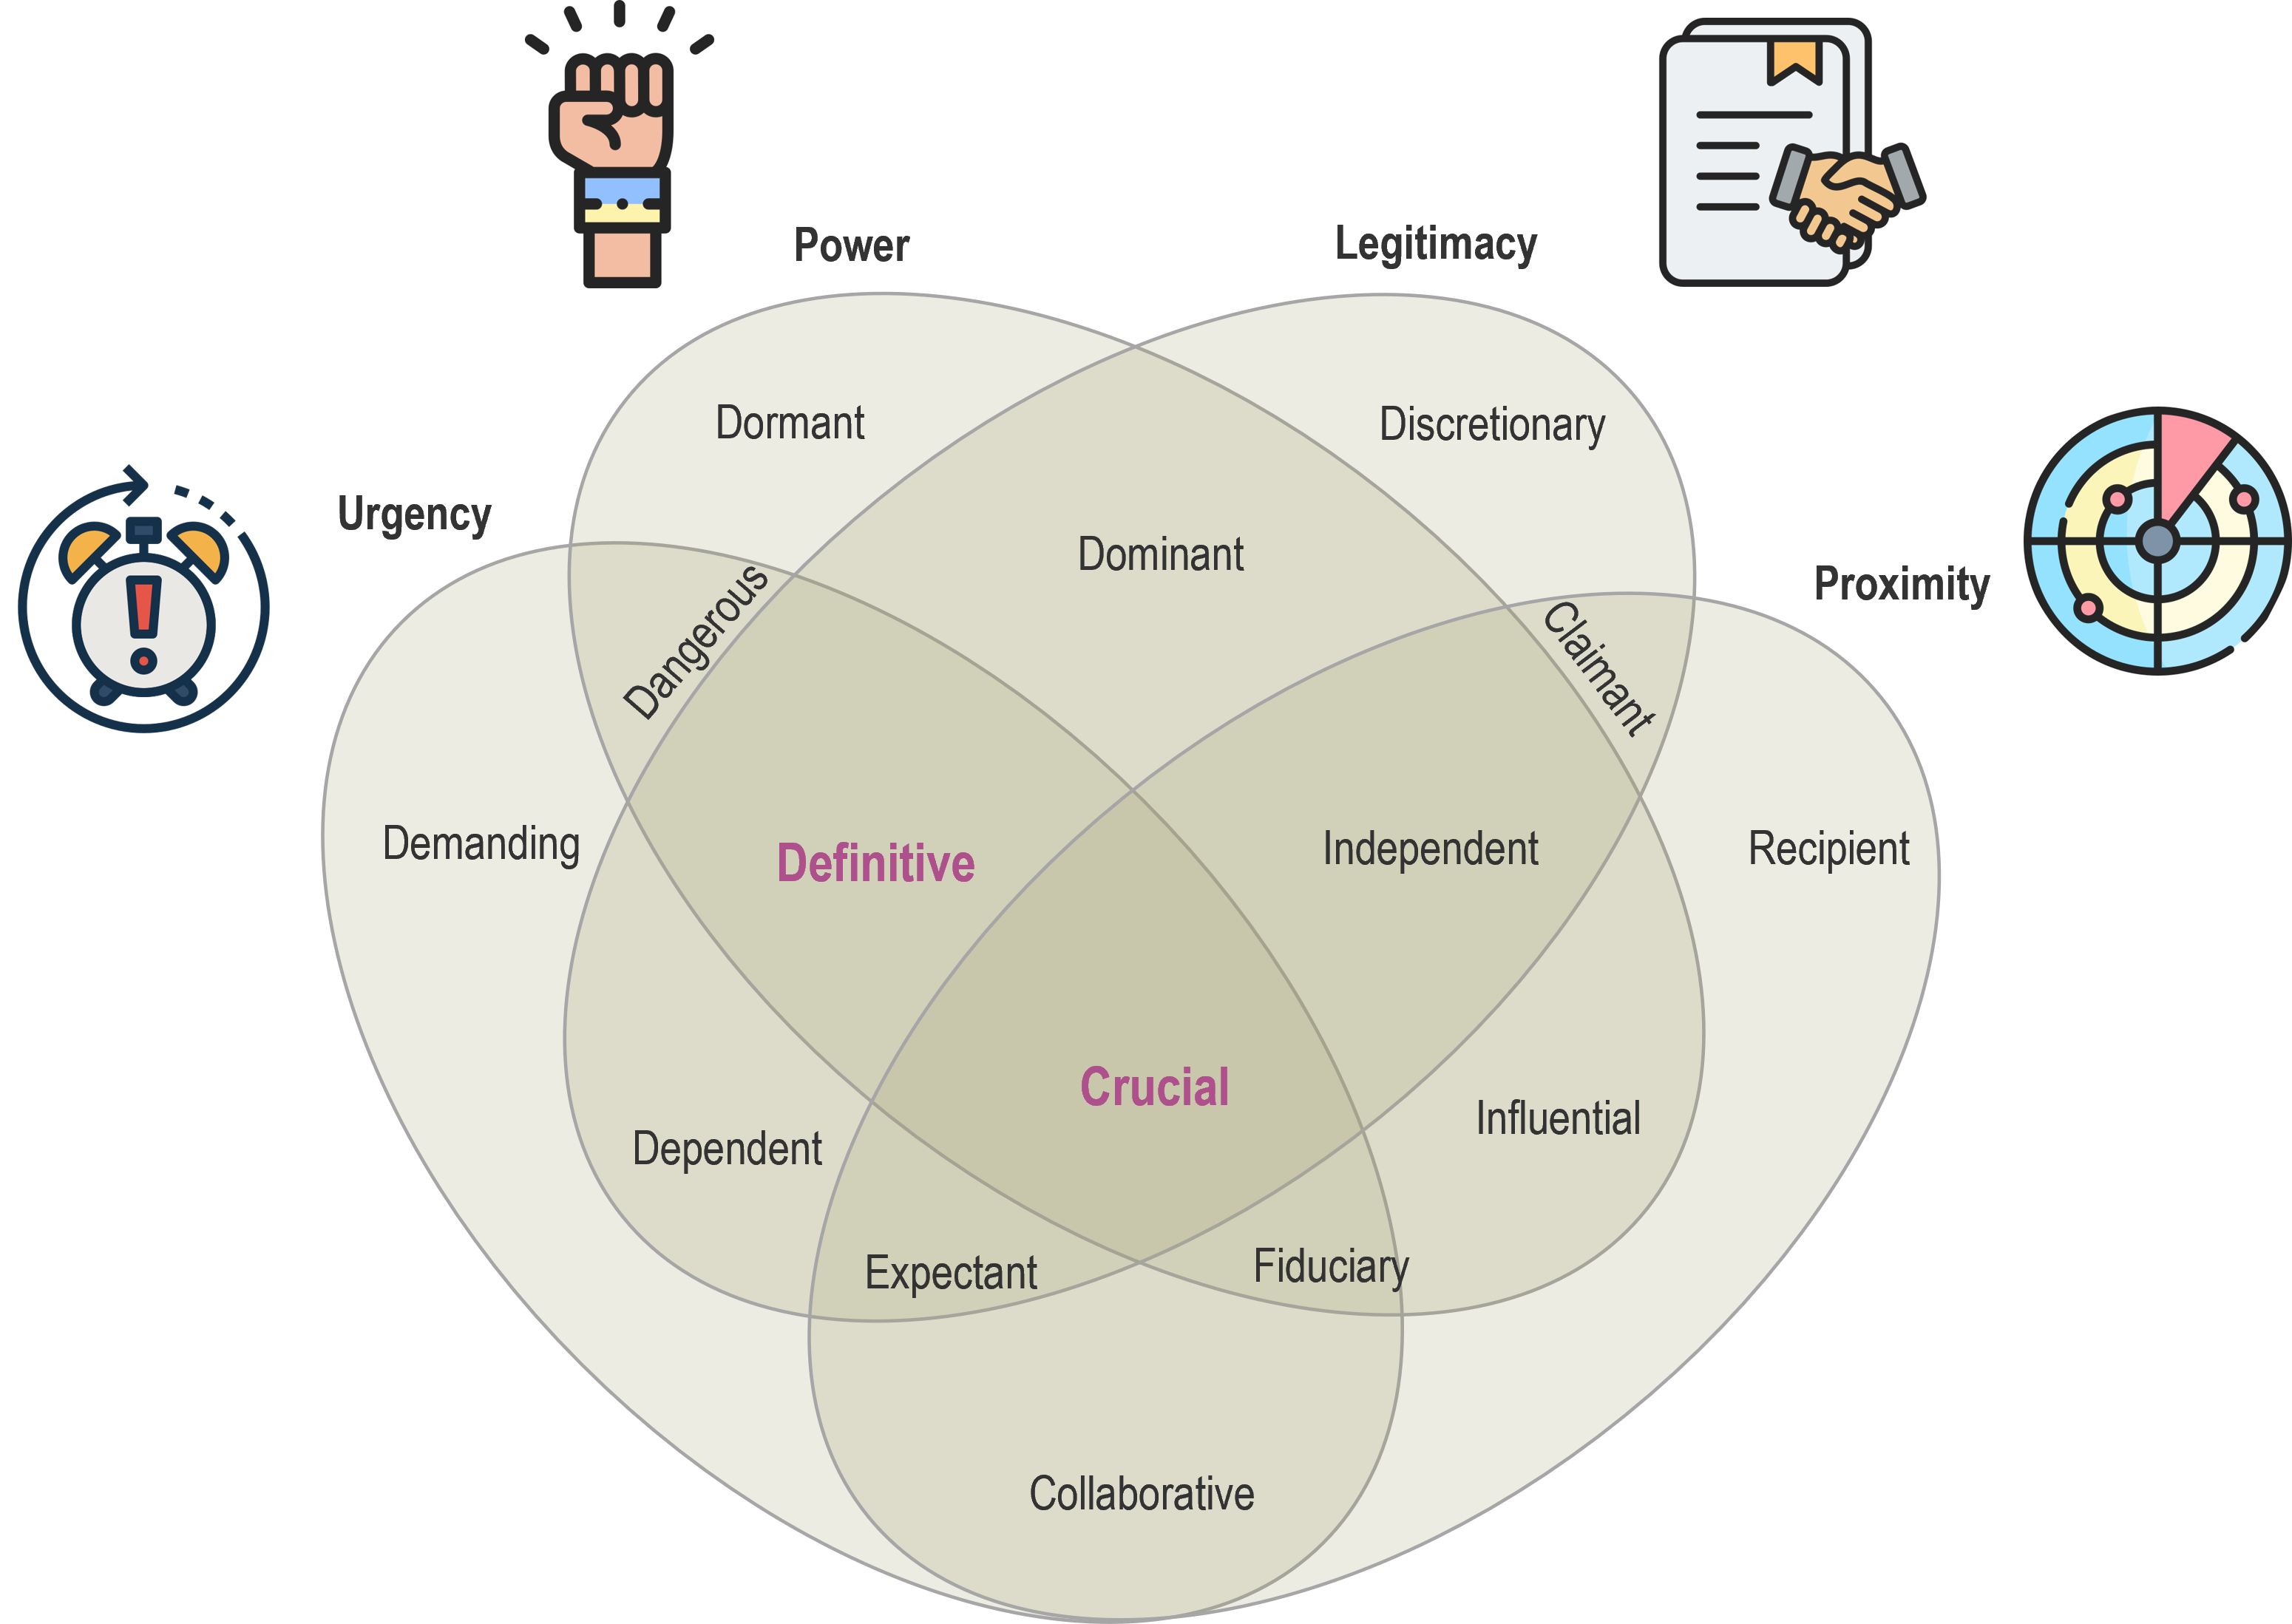
\includegraphics[width=0.8\columnwidth]{Figures/Shafique Stakeholders.png}
        \caption{Stakeholders' typology with four attributes and their relationships. Source: (Shafique \& Gabriel, 2022)}
        \label{fig:figure2}
    \end{figure}
    % \begin{table}[htb]
    %     \label{tab:table1}
    %     \centering
    %     \caption{Stakeholders' Typology, attributes, and description. Source: Shafique \& Gabriel (2022)}
    %     \todo[inline]{not sure if all of this is necessary for the paper or better to show the image}
    %     \begin{tabularx}{\columnwidth}{l X X}
    %         \toprule
    %         \#  & New Typology (Attributes) & Description \\
    %         \midrule
    %         4   & Recipient (Proximity) & Recipient stakeholders receive some benefit from the project because they reside in or close to the project implementation area. Although not the project's target beneficiaries, they benefit indirectly from it because of their physical closeness to its beneficial outcomes. \\
    %         7   & Claimant (Legitimacy \& Proximity)    & Claimant stakeholders have a perceived legitimate role and claim to the project and reside in or close to the project area. They receive a direct benefit from the project outcomes. \\
    %         9   & Influential (Power \& Proximity)  &  Influential stakeholders are powerful and either reside in or have some form of control over the project implementation area. \\
    %         10&Collaborative (Urgency \& Proximity) & Collaborative stakeholders do not possess power and legitimacy. However, because they were affected by the disaster due to their closeness to affected areas, they have a high interest in the urgent completion of the reconstruction project. Their collaboration contributes to the success of the project. \\
    %         12 & Independent (Power, Legitimacy \& Proximity) & Independent stakeholders can implement the project without the help of other stakeholders because of their ability to influence others and the official recognition of their role in implementation. These are usually local stakeholders with a physical presence in the project area \\
    %         13 & Expectant (Legitimacy, Urgency \& Proximity) & Expectant stakeholders are not considered powerful but expect to benefit directly from the project because they possess urgency, proximity, and legitimacy attributes. Other stakeholders (though not necessarily project implementers) recognize them as stakeholders, legitimizing their role. \\
    %         14 & Fiduciary (Power, Urgency \& Proximity) & If collaborative stakeholders acquire power over the project implementation area, they become fiduciary stakeholders. Project managers recognize their responsibility to report directly to these stakeholders on project outcomes. Vulnerable-affected communities might aspire to this role by demanding community-driven approaches to project implementation. \\
    %         15 & Crucial (Power, Legitimacy, Urgency \& Proximity) & Crucial stakeholders are the project's decision-makers, implementers, and beneficiaries. Possession of proximity attributes helps them gain direct benefits from the project. For vulnerable affected communities, the role of a crucial stakeholder is even better than that of a fiduciary stakeholder.\\
    %         \bottomrule
    %     \end{tabularx}
    % \end{table}
    
    This  salient model does not consider a method for identifying the possession of each attribute and the relationships between one and another stakeholder. Any classification, naturally, carries a research bias regarding stakeholder typologies and designations.

\subsection{Research Gap and Contribution}

As explained above,
    
    \section{Methods} \label{sec:Methods}
    Our UDT development process includes on-site and desktop geospatial data collection, stakeholder identification and prioritization, 3D city digital reconstruction, SW generation estimation, and optimal SW collection routes design. In the conclusion, we also include an assessment and reflection on the UDT process.
    \subsection{Study area} \label{subsec:Study Area}
    The study area (9.45 km$^2$) is the Hatfield and Hillcrest neighborhoods in Pretoria, City of Tshwane, South Africa. The area has various land uses, ranging from residential to agricultural, including the University of Pretoria campuses (See Figure \ref{fig:studyArea}). The area includes the Hatfield City Improvement District (CID), a private non-profit organization performing local urban management functions. The CID is taxpayer-funded through property levies which are collected by the municipality and transferred to the  CID to provide urban services (such as cleaning and maintaining public spaces, providing private security, or urban beautification) \citep{cidHatfieldCIDBrochure2021}.
    \begin{figure*}[h!]
        \centering
        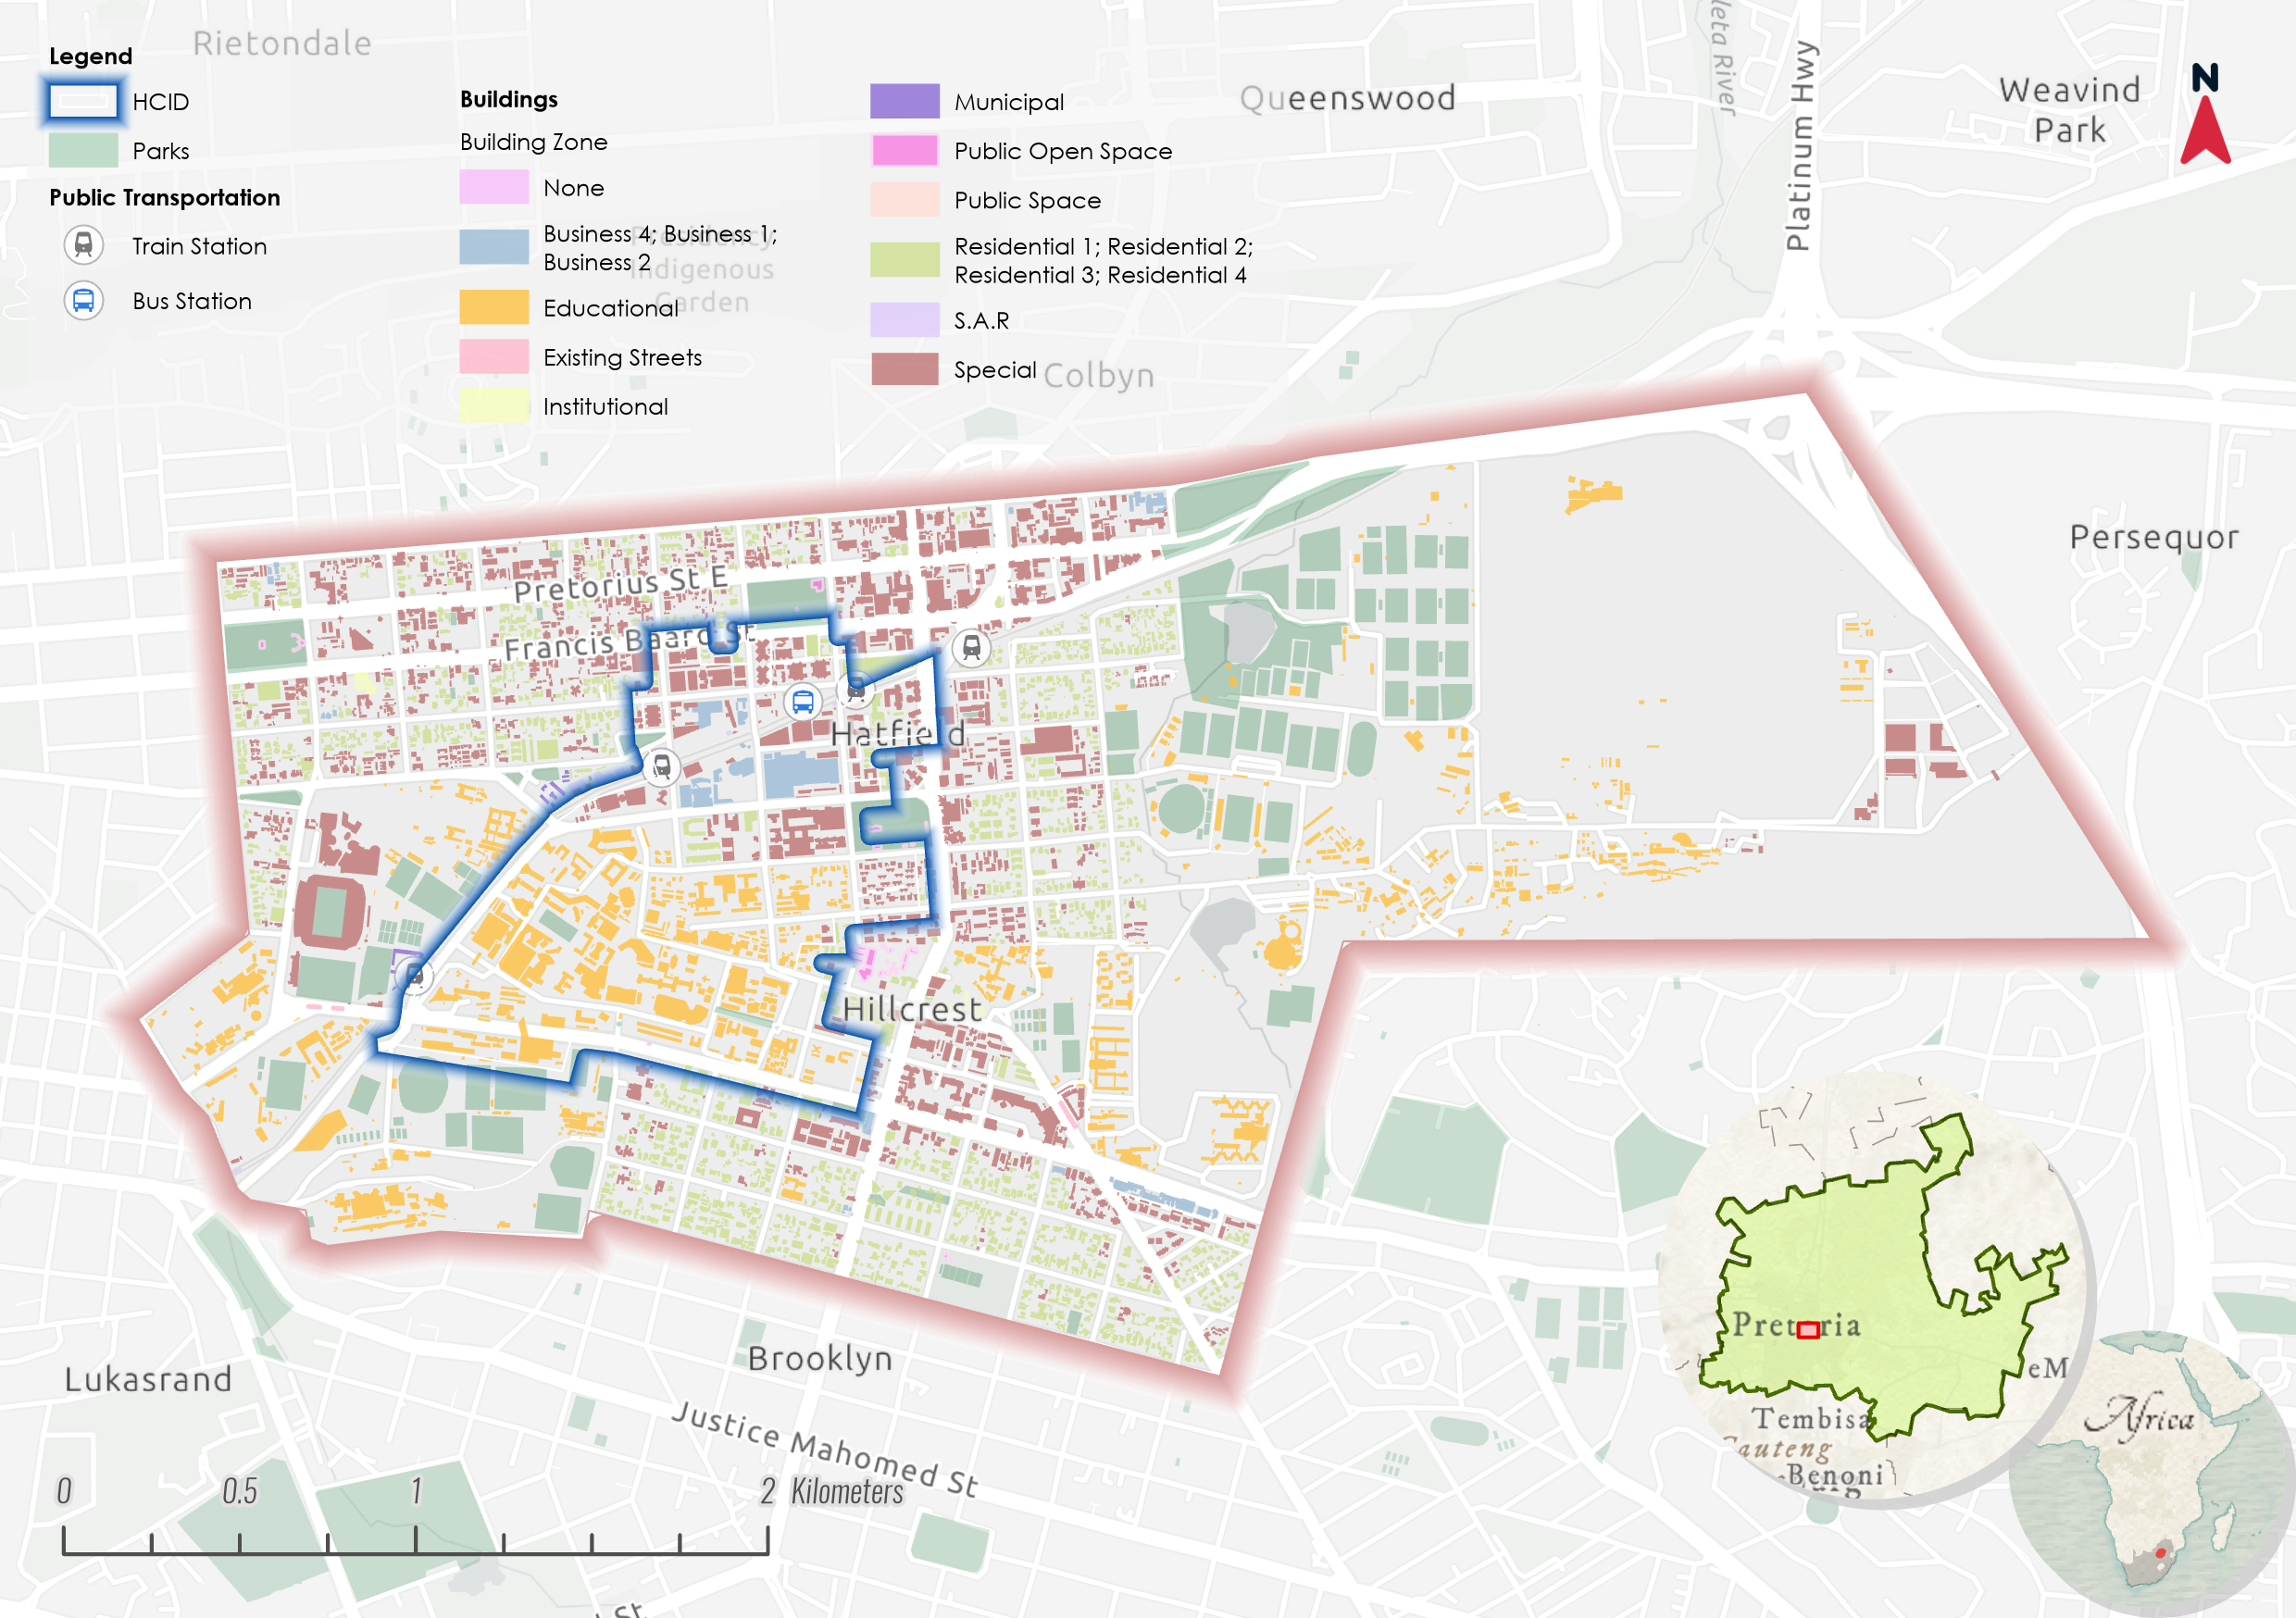
\includegraphics[width=\linewidth]{Figures/Study Area+HICD.png}
        \caption{Hatfield Digital Twin City Study Area.}
        \label{fig:studyArea}
    \end{figure*}
    \subsection{Geospatial datasets} \label{subsec:Geospatial}
    Our research uses geospatial data from CoT, the National Geo-Spatial Information Centre of South Africa, and data collected by the Department of Architecture at the University of Pretoria. The initial data is summarized in Table \ref{tab:Datasets}. For a web application, all data was reprojected to WGS 1984 (ESPG: 4326). Length and area attributes were calculated in Hartebeesthoek94 / Lo29 (ESPG: 2053).

    \begin{table*}[!h]
        \caption{Datasets used}
        \scriptsize
        \label{tab:Datasets}
        \begin{tabularx}{\textwidth}{X X X X X X}
            \toprule
            Geospatial Dataset & Specifications & Data Type & Date & \shortstack{Coordinate\\ System} & Source \\
            \midrule
            LIDAR Scanning & Aerial laser scanning with 0.6m of separation & LAS & June,2019&EPSG:4148&CoT GIS, ESRI \\\\
            Buildings&Building footprints with attributes Name,type of building&Vector Polygons& March,2023&EPSG: 4326&OpenStreetMaps Contribuitors\\\\
            Road Network&Polyline of motorcar roads, including total length, road direction, road type&Vector Lines&March, 2023&EPSG:2053&CoT GIS portal\\\\
            Aerial Imagery&Very High-Resolution Imagery from Unmanned aerial vehicles - UAV from the study area. RGB Bands. 0.1m Spatial Resolution&Raster&June,2018&EPSG:2053&CoT GIS Portal\\\\
            Zoning&Polygons Defining regulations for land use&Vector Polygons&March 2023&EPSG:2053&CoT GIS Portal\\\\
            Global Settlement Population&Estimated Residential population per 100x100m cell. Epoch 2020&Raster&June, 2022&EPSG:54009&GHS population grid multitemporal (1975-2030) \citep{Schiavina2022}\\\\
            Solid Waste Containers and Littering Location&1,270 containers and 820 illegal dumping reports &March,2023&EPSG:4326&Vector Point& On-field data collection - \citep{cardenasivanSolidWasteVirtual24}\\\\
            \bottomrule
        \end{tabularx}
    \end{table*}

\subsection{Urban waste management digital twin design} \label{subsec:Phase3}
    The UDT design requires a series of steps in digital city reconstruction, waste calculation, route optimization, and system integration.  Figure \ref{fig:flowchart}, shows a detailed flowchart summarizing the process.

    The UDT prototype is designed assumes a constant input of waste generation, which is simulated for this research, and an adaptative waste collection route. In this sense, the tool is design as a constant monitoring of waste management for operational improvement and reduction of human intervention
    
    \begin{figure*}[!h]
    \centering
        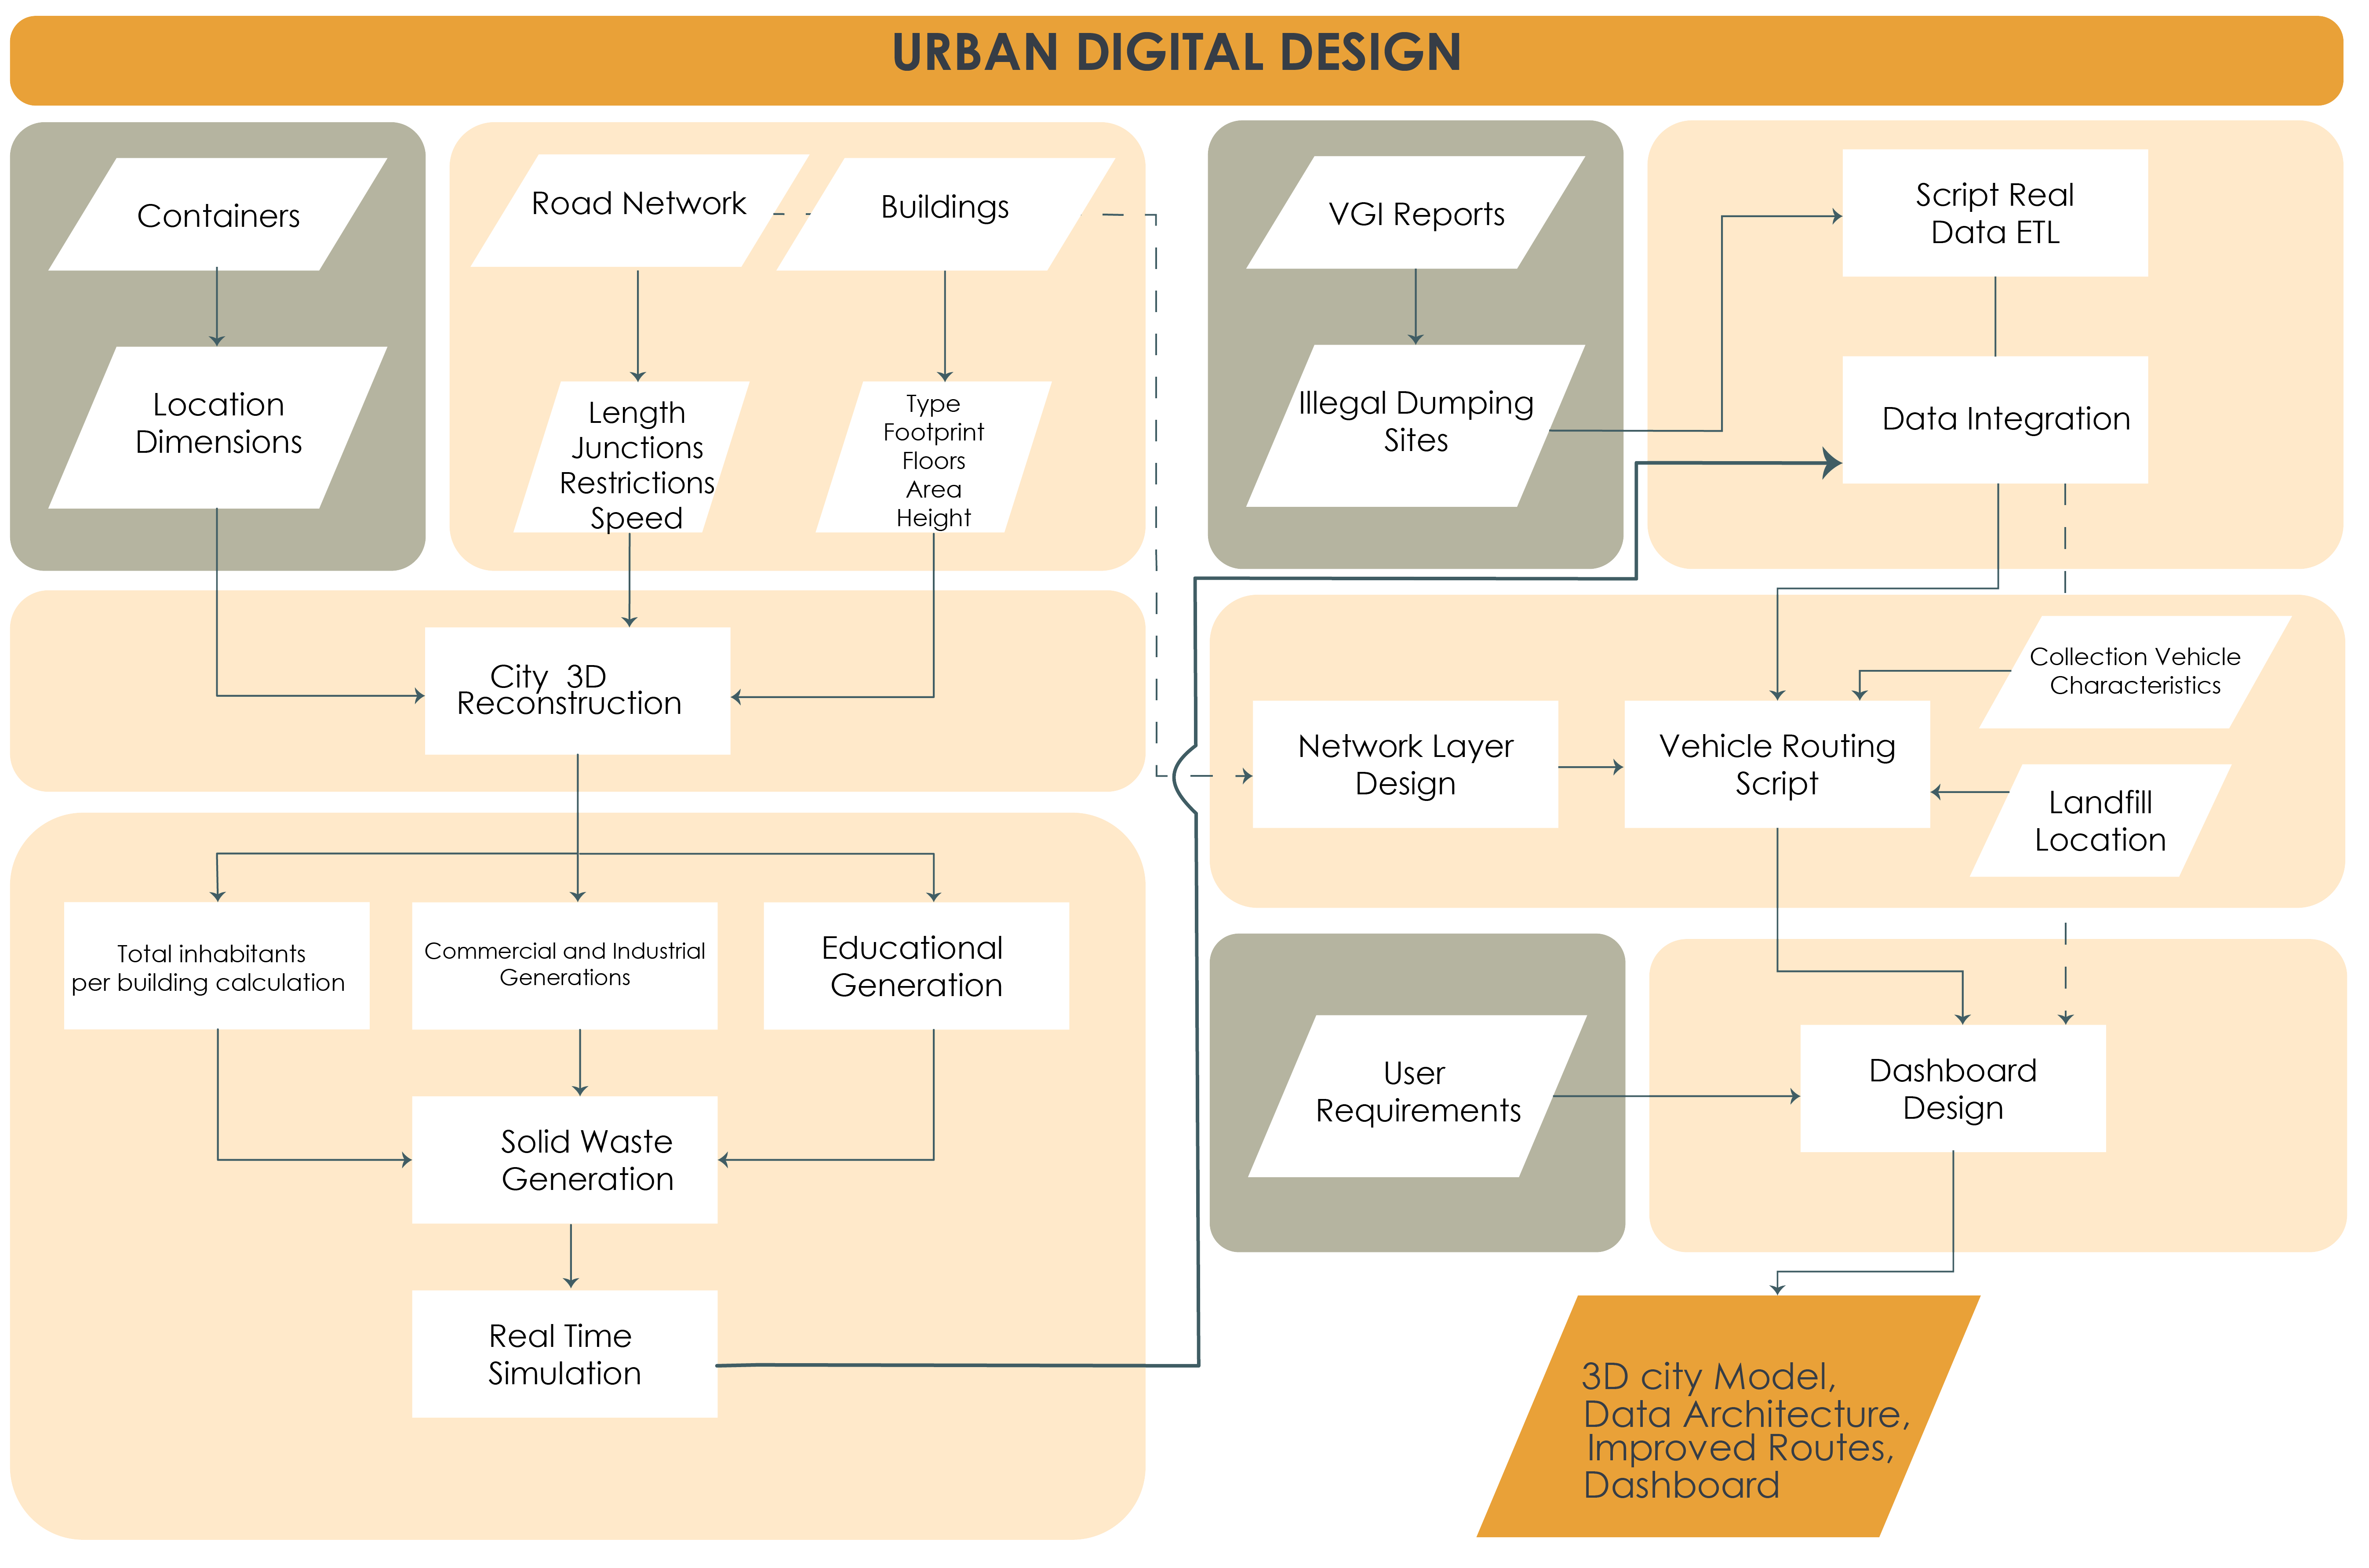
\includegraphics[width=1.2\linewidth]{Figures/Phase III_.png}
        \caption{Urban Digital Twin Design Flowchart.}
        \label{fig:flowchart}
    \end{figure*}

\subsubsection{Stakeholder identification} \label{subsec:stakeholderIdent}
   Stakeholders in this area often engaged in voluntary and open academic discussions about local city issues with students and teachers at the University of Pretoria. One academic discussion was held to unpack general ideas on improving local SW management. With voluntary consent, the discussion was recorded, transcribed, anonymized, and analyzed following a method developed by \citet{Radford2022}. The discussion was further analyzed to identify potential additional or missing stakeholders. The relationships of \textit{Power}, \textit{Urgency}, \textit{Legitimacy}, and \textit{Proximity} were classified and drawn according to the adapted salient model \citep{Mitchell1997, Shafique2022}.

    To further classify and reduce subjectivity, an Analytical Hierarchical Process (AHP) pairwise comparison was made \citep{Saaty1987, Saaty1990}. Each attribute was compared on a nine-point scale, where stakeholder \textit{i} is compared with stakeholder \textit{j} (Table \ref{tab:Saaty}).
    
    \begin{table}[h!]
        \centering
        \caption{Analythical Hierarchical Process pairwise comparison. Source: (T. L. Saaty, 1990)}
        \small
        \label{tab:Saaty}
        \begin{tabularx}{\linewidth}{X c}
            \toprule
            Relative Importance&Definition – X: Power, Urgency, Legitimacy, Proximity\\
            \midrule
            1&\textit{i} and \textit{j} have equal X\\
            3&\textit{i} have moderate X over \textit{j}\\
            5&\textit{i} have strong X over \textit{j}\\
            7&\textit{i} have very strong X over \textit{j}\\
            9&\textit{i} have extreme X importance over \textit{j}\\
            2,4,6,8&Intermediate values between two adjacent judgments\\
            Reciprocal&When the relation is inverse –
            (eg. \textit{j} has strong X over \textit{i}: 1/5)\\
            \bottomrule        
        \end{tabularx}
    \end{table}
    
    A comparison matrix was generated, values were normalized, and, based on the resultant eigenvector of each attribute, the stakeholders were classified according to the adapted salience model types. From this result, \textit{Definitive} and \textit{Crucial} stakeholders were considered the primary end-users of the UDT.

    \subsubsection{System architecture and data integration}\label{subsubsec:SystemArch}
    Integrating the elements into one Digital Twin followed the architecture proposed in Figure \ref{fig:architecture}. The process includes retrieving citizens' collected data through Epicollect5 API, exporting data to a JSON file, filtering and transforming data into a CSV point file, and converting the point layer to visualize SW containers. SW containers were allocated to buildings using a near function. The optimal route for waste collection vehicles is calculated using the ArcPy routing module and resulting routes and pick-up sequences are displayed in an online operational dashboard, updating every 6 seconds. The online dashboard contains important descriptive statistics and key requirements identified by stakeholders (see section \ref{subsec:stakeholderIdent}). The whole system was assembled in a local setup with a computer featuring 28 GB RAM, 3.8 GHz - 8 cores – 16 threads CPU, and 4 GB dedicated GPU; and also a  Cloud service using  ArcGIS server
with 64 GB RAM, 2.1 GHz - 8 cores – 16 threads CPU, and no GPU.


    
       \begin{figure*}[h]
       \centering
    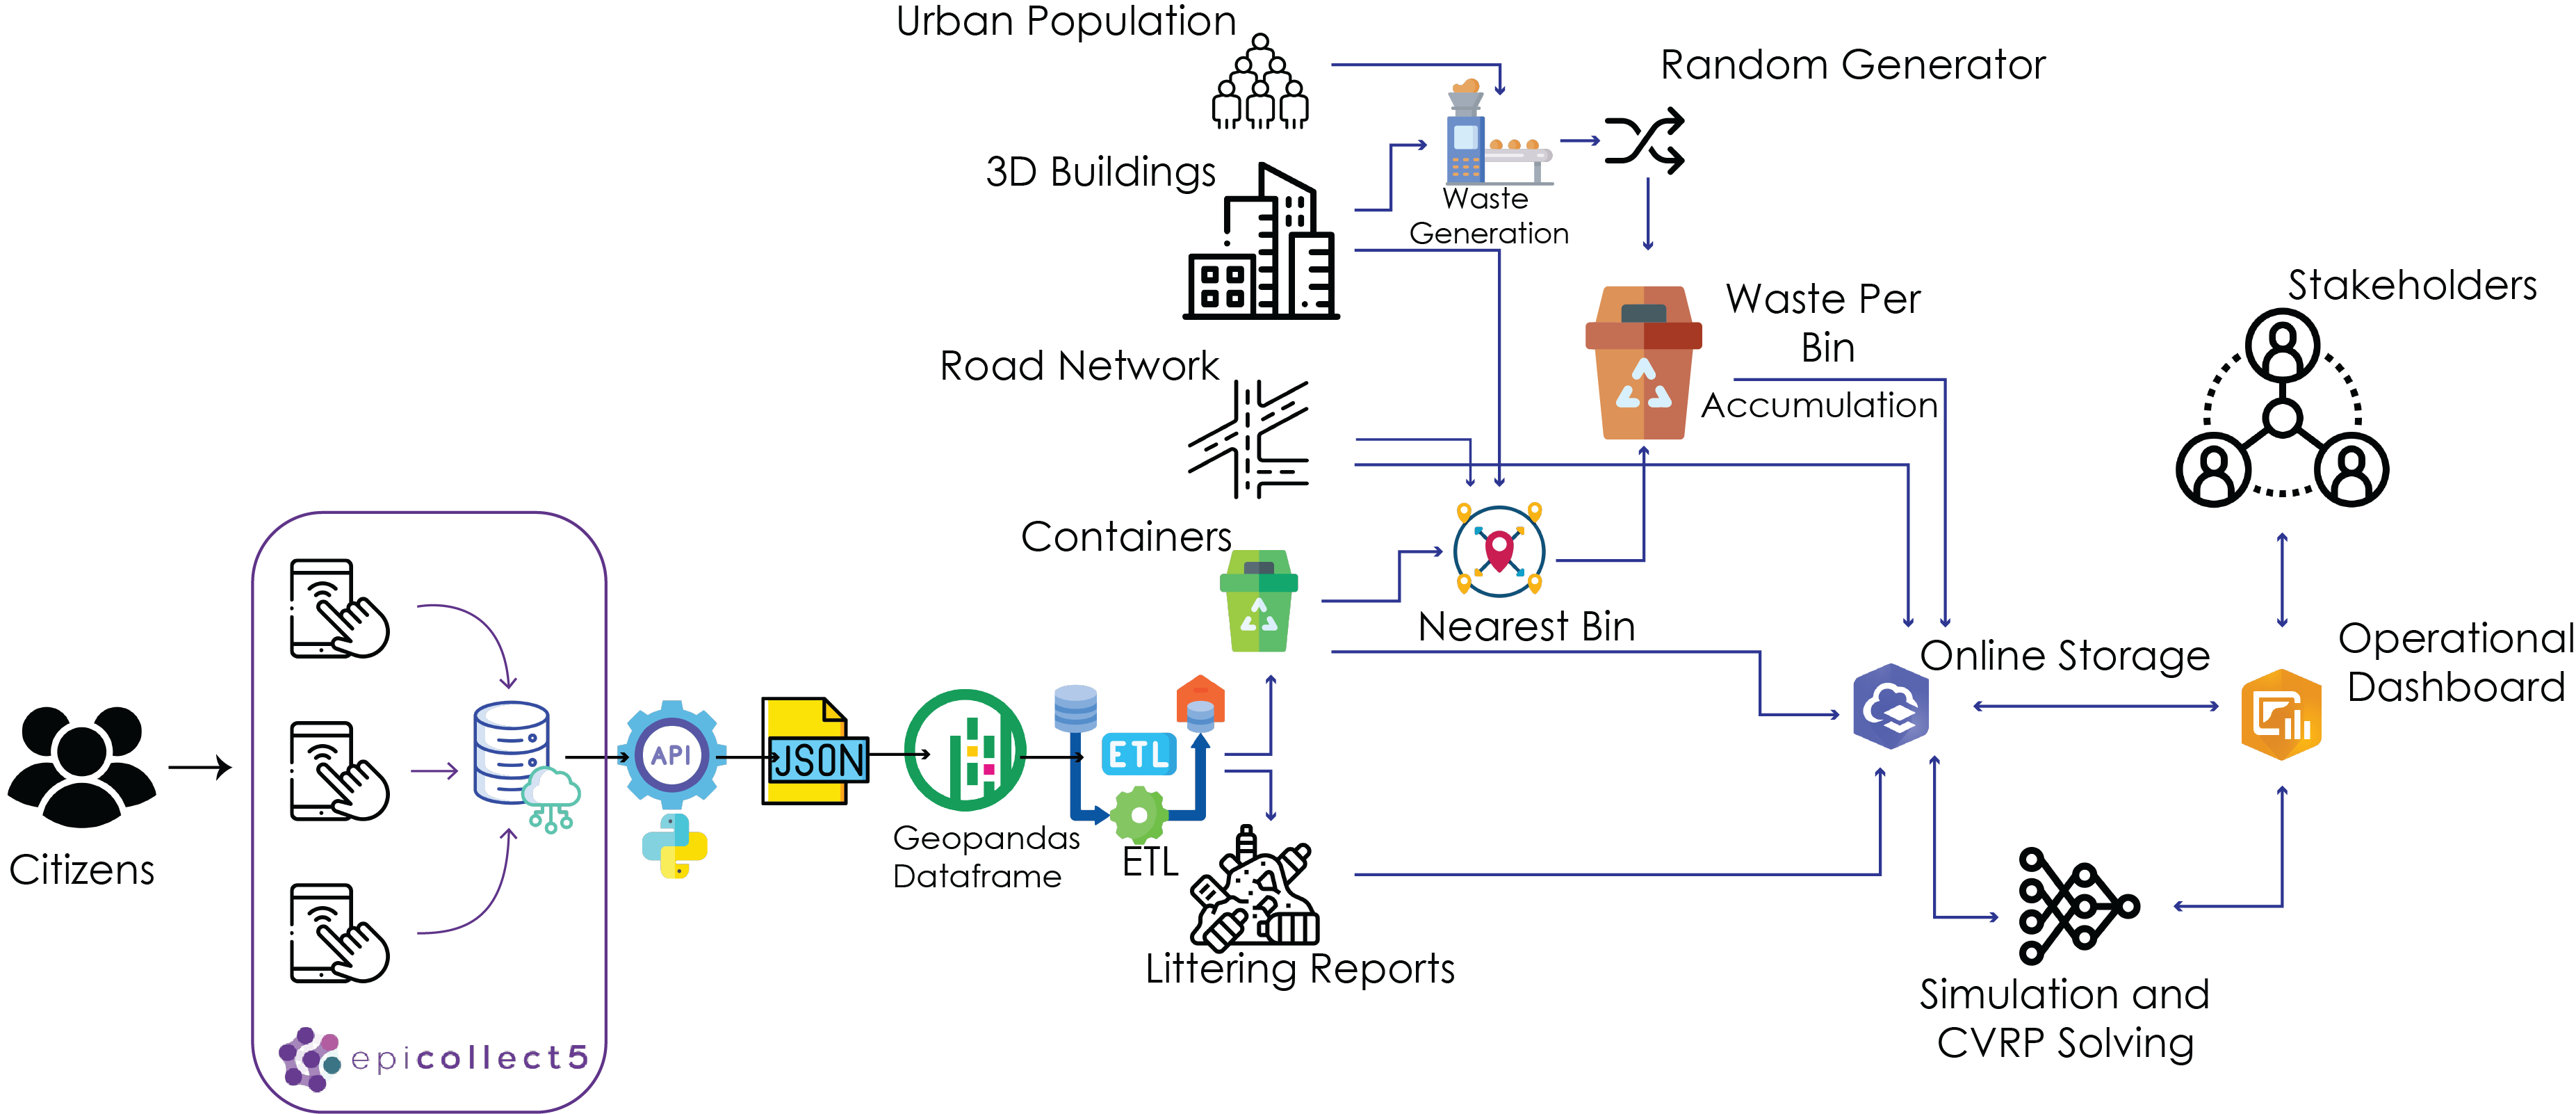
\includegraphics[width=1.2\textwidth]{Figures/System Architecture.png}
        \caption{Waste Digital Twin Architecture}
        \label{fig:architecture}
    \end{figure*}

    % \subsubsection{City buildings reconstruction} \label{subsubsec:Buildings}
    % City buildings were reconstructed using aerial LiDAR scanning data acquired in  June 2019 and classified into five categories: ground, noise, low-vegetation, high-vegetation, and building points. OpenStreetMap (OSM) building footprints \citep{contributorsPlanetDumpRetrieved2023} were used to improve building classification by performing 2D intersections, further differentiating vegetation from buildings. The building points were transformed into a flat raster (no Z-values), and void areas were filled in at a distance of 1.2m (double the pixel size of the LiDAR scan). The resulting raster was transformed into polygons. Edge angles were normalized into right angles and diagonals to obtain geometrically valid polygons. The final polygons were checked with the OSM to extract missing building footprints. The footprints were merged into a single file containing complete building footprints of the study area. The quality of the result was tested with a confusion matrix analyzing 1,000 random point locations in the study area. 

    % From the ground classification of the LiDAR point cloud, a Digital Terrain Model, Digital Surface Model, and Normalized Digital Surface Model were generated. Together with the building footprints, these were used to extract the base elevation of the buildings and average height. To improve quality, polygons with areas $<25m^2$ and heights $>3m$ were identified and visually inspected to detect and eliminate false positive results (generally related to trees).

    % CityGML 3.0 model attributes, namely, \textit{number of stories above ground, class, function, }and\textit{ usage} were used to add extensive building attribute information, support classification, and produce waste generation estimates. Individual building data was obtained by combining OSM information, CoT zoning \citep{tshwaneGeographicInformationSystem2023}, and on-field validation of the building attributes, performed by a group of undergraduate architecture students at the university. For each building, the total estimated floor area was calculated by dividing building height by 2.4m (the minimum required room heights in the city) \citep{tshwaneTshwaneTownplanningScheme2014}, and multiplying this with the footprint area to obtain the total estimated floor area. Where on-field validation was impossible, a UAV Image was used to perform quality control in classifying buildings and determining their usage. 

    \subsubsection{Solid waste generation calculation} \label{subsubsec:Generation}
    For residential population estimation, we used the Global Human Settlement Population Layer \citep{Schiavina2022} on a 100m resolution. We calculate population density per pixel based on each polygon's total floor area of residential buildings. We used the population density value to derive an estimated population count for each residential building. This was multiplied by an average waste production value, allowing us to estimate the daily waste production per building.
   
    Non-residential buildings were categorized into four classes (see Table \ref{tab:waste1}) ordered by high-to-low SW generation rates. We selected the upper tier value of the SW generation range, as indicated by \citet{Karadimas2008} as there are limitations on local SW production per type of building or economic activity.

    \begin{table*}[h!]
        \centering
        \caption{Building classes, related commercial activity, and waste production. Source: adapted from Karadimas \& Loumos, 2008.}
        \footnotesize
        \label{tab:waste1}
        \begin{tabularx}{\linewidth}{l X r}
            \toprule
            Category&Typical Commercial Activity&\shortstack{Waste production \\
            $(kg/m^2 - d)$}\\
            \midrule
            A& Supermarket, bakery, restaurant, grocery store, greengrocery store, fish store, fast food, bar, pub, club, café.&0.419\\
            B& Butcher store, patisserie, hairdresser, wine-vault, floristry, garage, pizzeria.&0.225\\
            C& Theatre, church, school, bookstore, barbershop, traditional café, pharmacy, post office, lingerie.&0.124\\
            D& Embassy, office, Insurance company, chapel, betting shop, tutoring center, shoe store, clothing store, jewelry store, video club.&0.024\\
            \bottomrule        
        \end{tabularx}
    \end{table*}

    For each building and its closest container, we used an “as-the-crow-flies” method to indicate where SW might likely be deposited and collected. We assigned a 600kg/m3 waste density per container based on the local collection company's operational estimation for the current routing scheme. To simulate waste production at each location, a random number between 0 and 1/24th of the total daily production was generated, and a maximum excess of daily waste production was set to 20\%.

    \subsubsection{Optimal Collection Route} \label{subsec:OptimalR}
    A network analysis was performed using a Capacitated Vehicle Routing problem solver \citep{ESRI2023c} to calculate optimal collection routes. The route solution model has several factors, including the aggregated containers’ locations, current volumes and levels, and vehicle capacity limits.

    %The solver uses a nearest insertion heuristics algorithm combined with the Tabú search meta-heuristic method \citep{ESRI2023a}. Such algorithms explores iterative solutions by moving between neighbors to find the best overall result. \citep{Avdoshin2019, Laporte2014}.  In nearest insertion, the algorithm picks the shortest edge and adds consecutive nodes to the solution where the total distance is minimized. \citep{Nilsson2003}. The Tabú search method allows moves with a negative gain if a positive has not been found. The algorithm creates a list of illegal moves to avoid infinite circular loops. Once a neighbouring solution is chosen, it will be added to the tabu list, ensuring that it is not revisited unless it leads to an improved tour or is removed from the list (\textit{ibid}).

    For this study, the road vector layer was first classified to identify directional segments and their categories (residential, highway, road-link) and vehicle speed restrictions. Next, a Network Analysis layer was created to identify edges and nodes, with edge weights calculated based on travel time using maximum speed and segment length. Containers with saturation over 75\% were selected and loaded into the network as collection orders.

    Analysis start- and end-conditions were set, waste accumulation simulations occurred, and network problem-solving occurred every sixth waste generation iteration (skipping the 24th for non-working hours). The solution involved creating an OD matrix representing the shortest path between collection orders and the landfill location, with collection orders added sequentially to optimize routes using a Tabú search meta-heuristic approached \citep{ESRI2023c}.

    After each solution, collected waste containers and saturation levels were reset, and non-collected orders continued accumulating until reaching the threshold. Routes and orders were, then, deleted to accommodate new routes and prevent processing memory overload.

    \subsection{Stakeholder Assesment} \label{sub:MethAssesment}

    This UDT development took place from Jan 2023 - June 2023. A UDT demonstration was conducted in July with 21 voluntary participants, showcasing the UDT dashboard's visualization and operating capabilities, and various data interactions. The demonstration included an overview of the UDT's development process, complemented by a demonstration video (see \ref{fig:video}). After the video, participants freely explored the tool and provided feedback through a simple voluntary and anonymous questionnaire.

    \begin{figure}[!ht]
        \centering
        
\includegraphics[width=\linewidth]{Figures/video.png}
        \caption{Demonstration Video Urban Digital Twin for Solid Waste Management - \href{https://www.youtube.com/embed/6k209psuRqw}{https://www.youtube.com/embed/6k209psuRqw}}
        \label{fig:video}
    \end{figure}

    The questionnaire, utilizing a five-point Likert scale, was designed to assess user satisfaction, usability, and usefulness based on the methods proposed by \citet{Ballatore2020} and the added value analysis by Pelzer \citep{Pelzer2014} (See Figure \ref{fig:AssesmentFr}). The UDT was evaluated and discussed following the three classes (purpose, trust, and function) of the Gemini Principles \citep{aGeminiPrinciplesGuiding2018}, as seen in Figure \ref{fig:DTPrinciples}.

    \begin{figure}[H]    
    \centering
    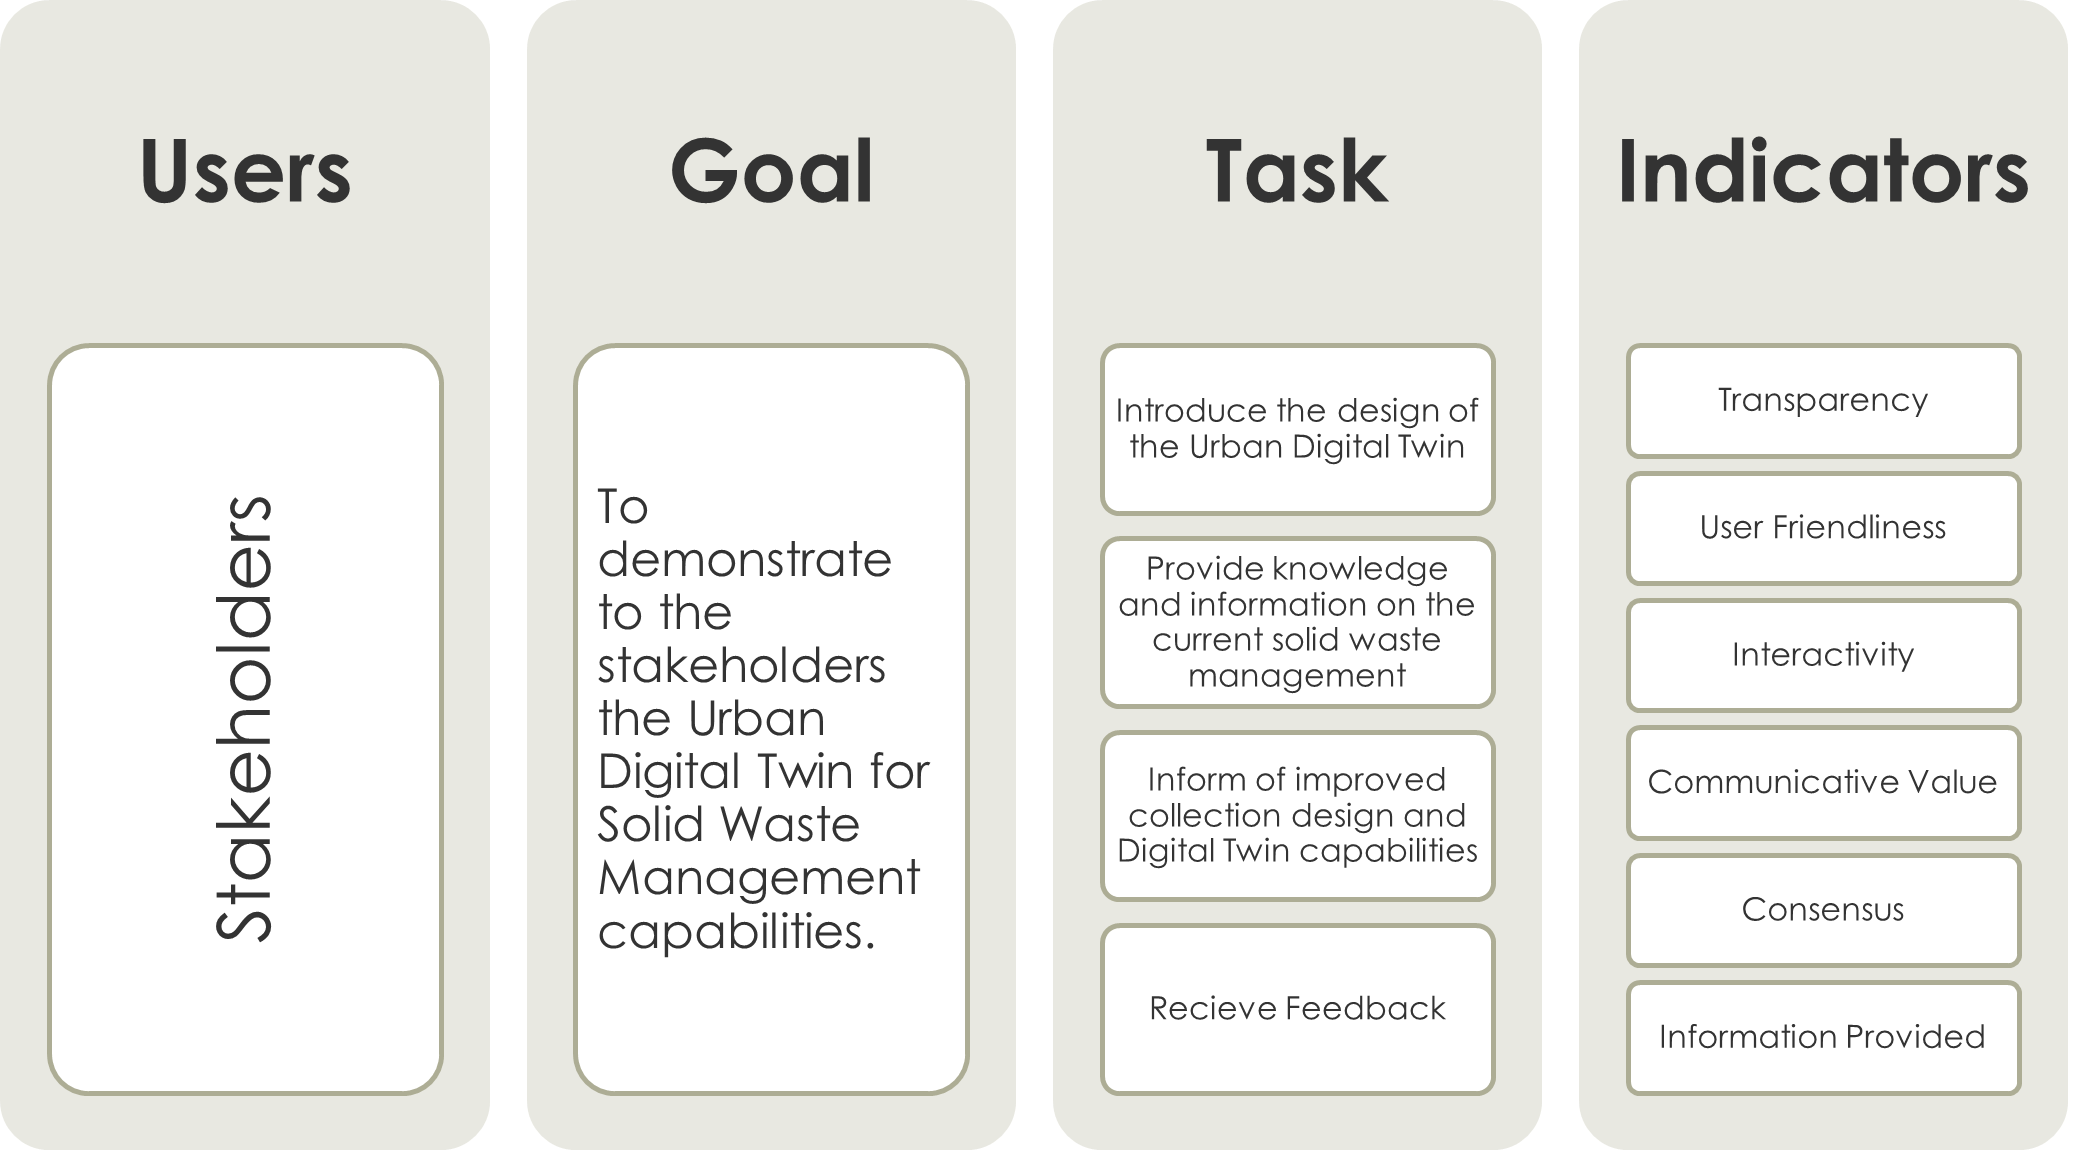
\includegraphics[width=\linewidth]{Figures/AssesmentFr.png}
        \caption{Assessment Framework.
        Source: adaptation (Aguilar et al., 2021 ; Ballatore et al., 2020 ; Pelzer et al., 2014)}
        \label{fig:AssesmentFr}
    \end{figure}

    \begin{figure}[H]
    \centering
    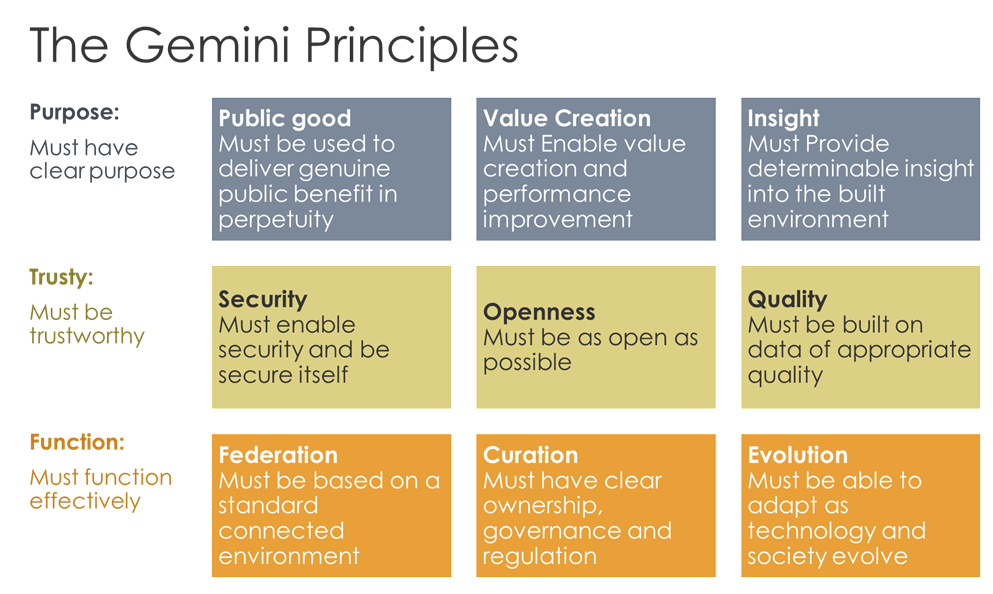
\includegraphics[width=0.8\linewidth]{Figures/Gemini.png}
        \caption{Digital Twins Gemini Principles. Source: (Bolton A \& Schooling, 2018)}
        \label{fig:DTPrinciples}
    \end{figure}

    \section{Results}
    \subsection{Current Practices}
According to the Community Survey Report of the Province of Gauteng \citep{africaProvincialProfileGauteng2018}, the CoT had 2,921,488 inhabitants in 2011 and 3,275,152 in 2016, reflecting an average annual growth rate of 2.28\%. Extrapolating with the same growth rate, the estimated population for 2023 is approximately 3,835,010 inhabitants.

 The 2011 census shows that the CoT had an urbanization level of 92.3\% \citep{africaCensus20112012}. Assuming no significant change in urbanization levels, the total population in the urban area of Tshwane is estimated to be 3,539,714 inhabitants in 2023 \footnote{After this research was completed, Statistics South Africa released the 2022/2023 Census. The total population of CoT is estimated to be 4.040.315 inhabitants; no specification on the urban-rural composition was made \citep{statisticssouthafricaCensus202223}.
 }. At a rate of 1.95 kg/inhabitant/day \citep{tshwaneCityTshwane20222022}, the estimated total production is 6,902.44 Tons/day for residential, commercial, and industrial waste.

The stakeholder discussions offer insights into the city's waste collection processes. The municipality collects waste weekly with $18m^3$ compacter vehicles with an efficiency of 4km/L of diesel. Each suburb has a designated collection day; collection companies only manage building types and residential unit counts. Due to high waste production, restaurants have a daily waste collection. Additionally, individual businesses can contract private waste collection companies to meet their specific needs. The municipality employs a team of foot workers in public areas to address pedestrian and vehicle littering. Equipped with bags for litter collection, they transport the collected waste to central points for truck pickup. Unlike scheduled truck collections, foot personnel operate on an "as-needed" basis

The CID provides an additional public space litter-picking service with 16-foot workers and one truck. %They receive 70,000 to 80,000 garbage bags annually from the municipality, and collection activities are logged manually by workers and their supervisors.
Foot workers adhere to a standardized schedule, picking litter in their designated area from 7 AM to 11 AM, covering approximately 1 to 1.5 blocks each. In the afternoon, they focus on tree maintenance and biowaste cleanup. During city events, in commercial streets (where bars and restaurants are located), or after weekends, workers concentrate on event areas before resuming regular duties. Private student accommodations, housing approximately 30,000 students, have their private waste collection using small trucks.

Various collectors in the city transport the waste to five existing landfills. Typically, waste is taken to the nearest landfill. In the Hatfield study area, this is the Hatherley Municipal Dumping Site located at 28.407°E - 25.741S %(Figure \ref{fig:landfill}).
At these sites, trucks unload waste as directed by supervisors and compact it when necessary. Landfills are open to the public for discarding various materials, including construction waste, electrical appliances, or bio-degradable waste.

    % \begin{figure*}[!ht]
    % \centering
    % 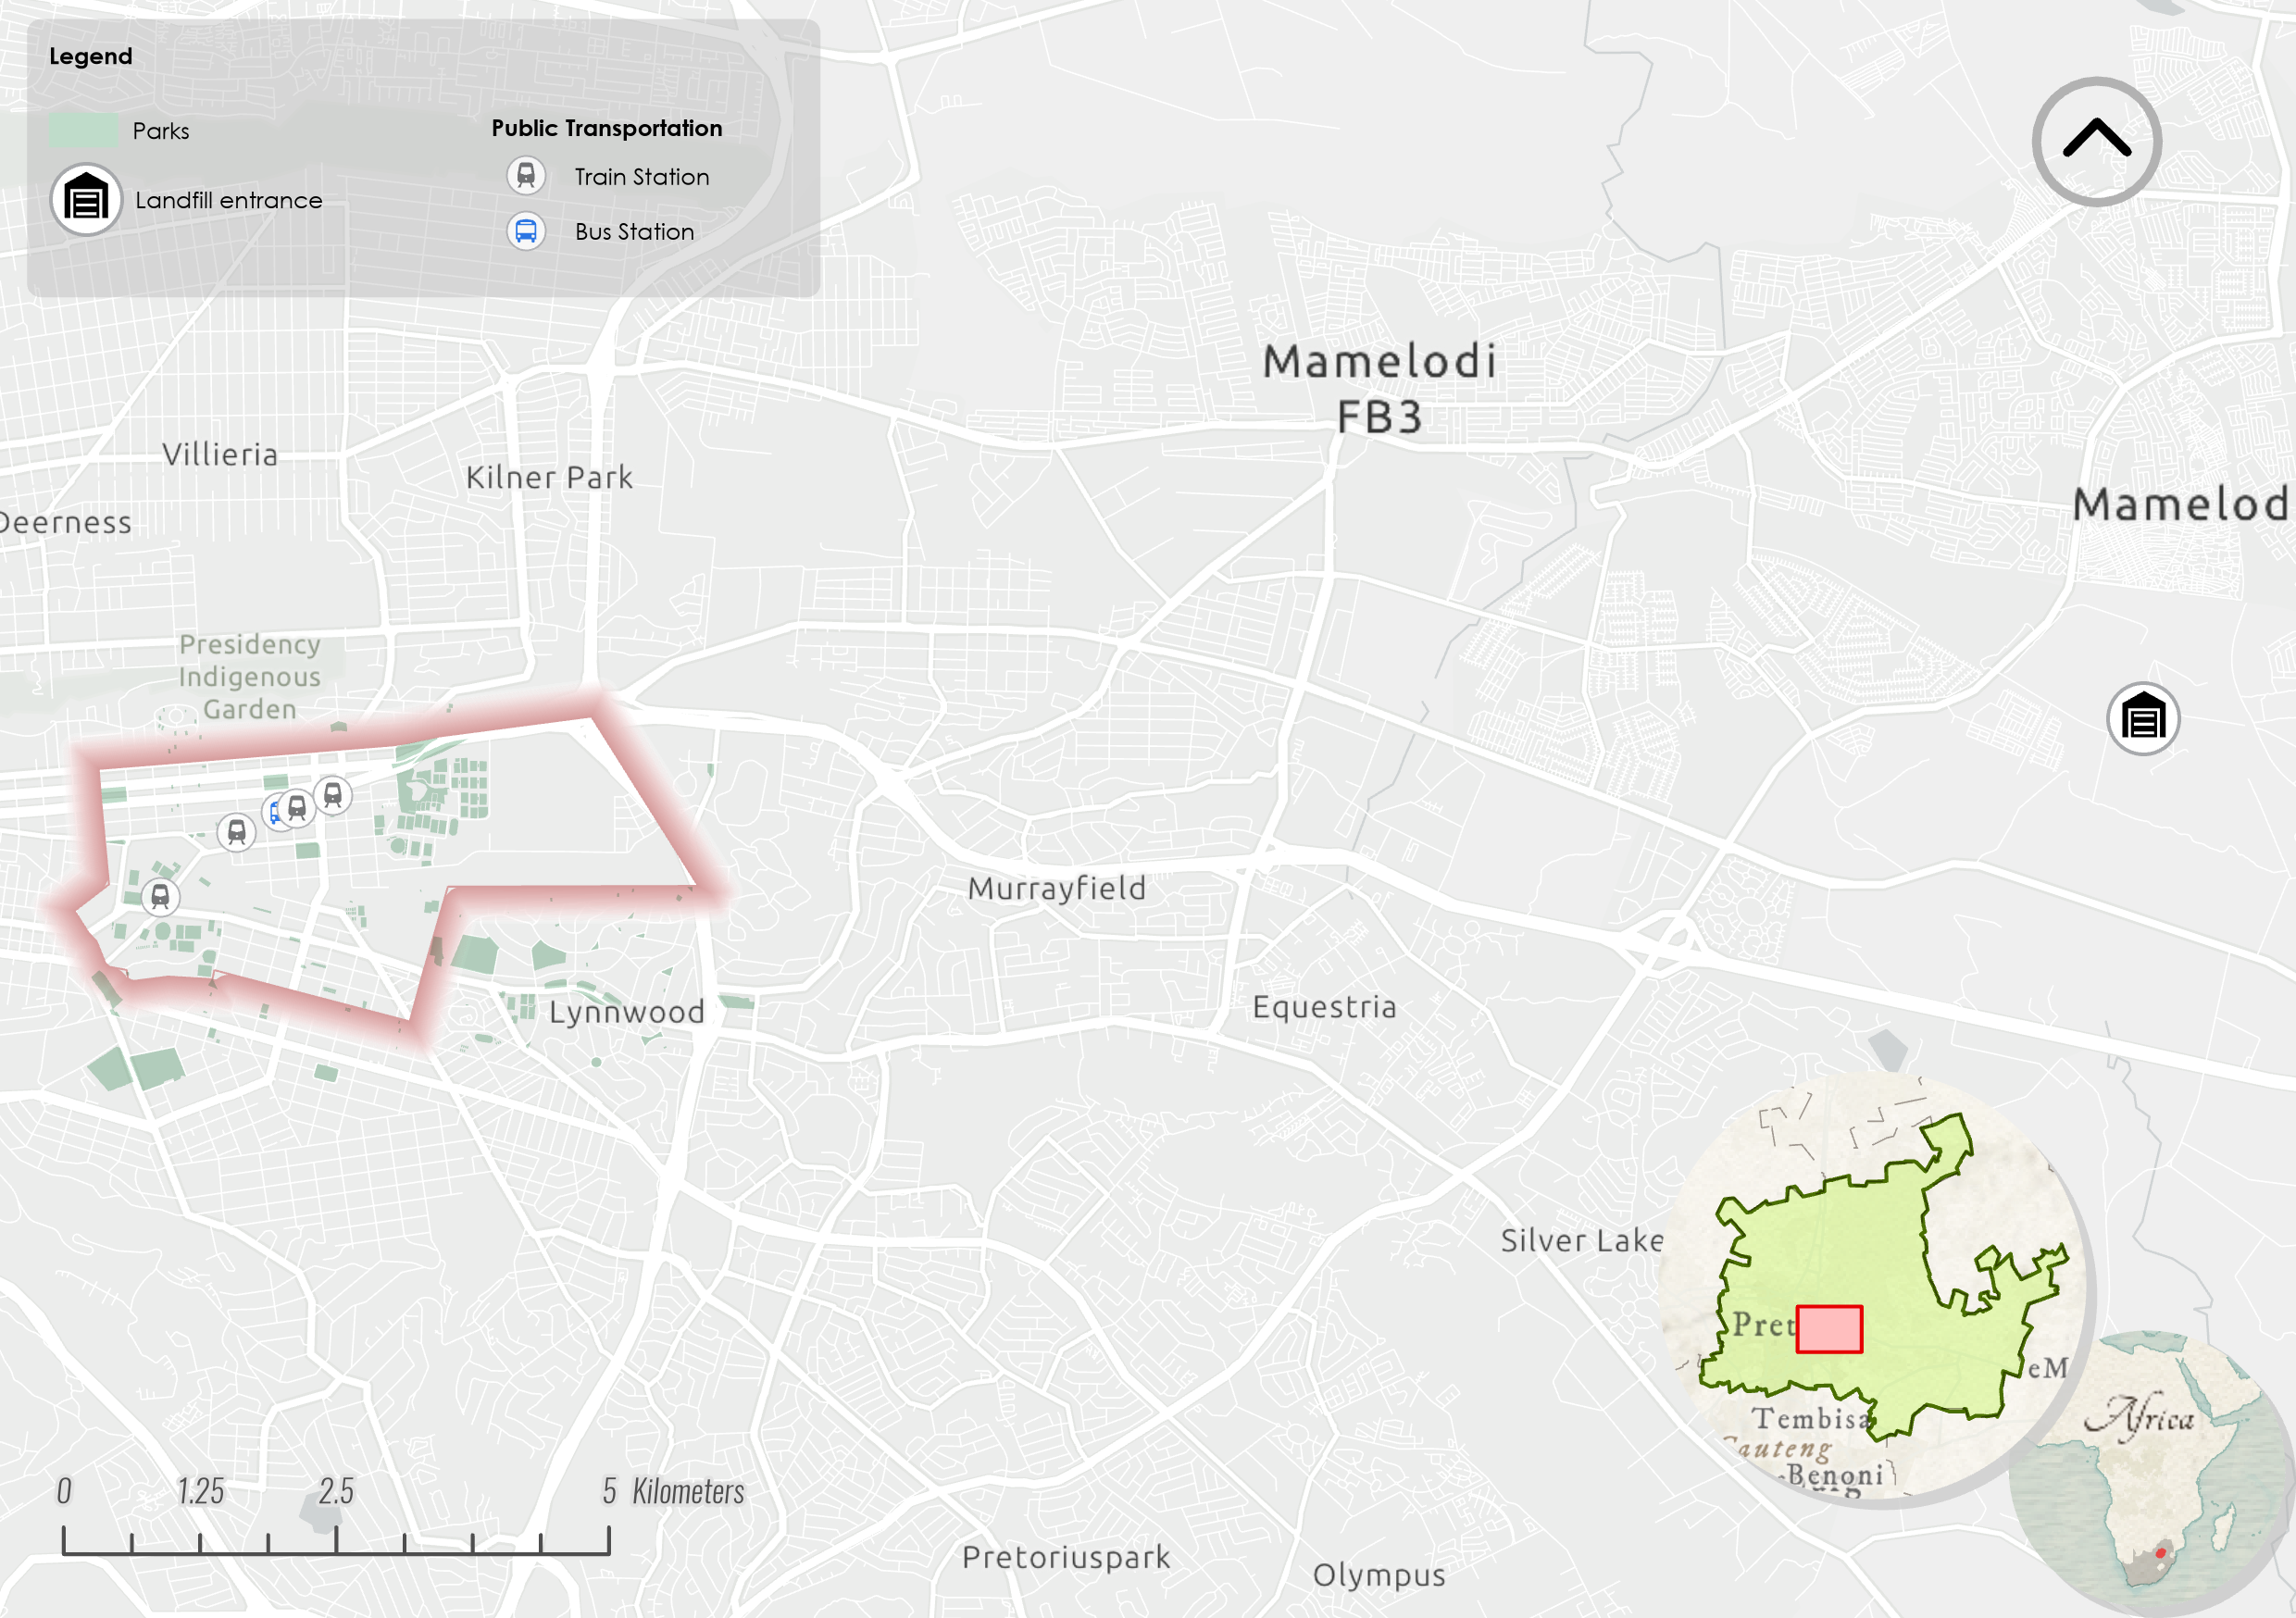
\includegraphics[width=\linewidth]{Figures/Landfill_Entrance.png}
    %     \caption{Hatherley Municipal Dumping Site location in relation to the study area}
    %     \label{fig:landfill}
    % \end{figure*}

    % \subsection{Stakeholder classification and system requirements} \label{subsec:Classification}

    Through stakeholder and academic discussions, 15 stakeholders were identified. After analyzing the anonymous transcripts, four pairwise comparison matrices were created for the four analyzed attributes and classified into typologies, shown in Table \ref{tab:stakeholderTyp}. %For this UDT prototype, three non-stakeholders were identified: local researchers, student residence managers, and compost providers.

    \begin{table*}[h!]
    \centering
        \caption{Stakeholders' attributes and typologies. Attribute values are percentage weights for each attribute calculated. Bold numbers indicate the largest weight for each attribute, and blue numbers indicate the lowest weight for each attribute. Typologies highlighted in purple are the stakeholders considered a primary focus for compliance with user requirements.}
        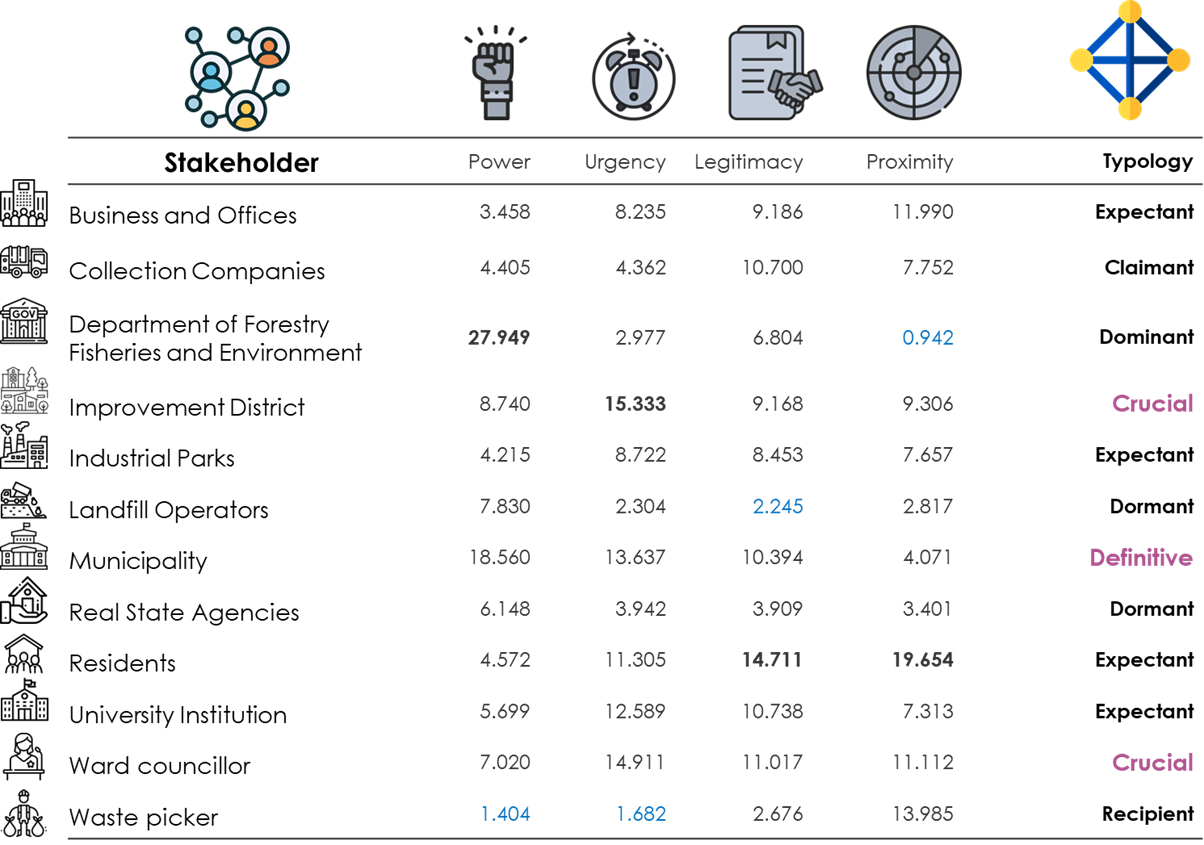
\includegraphics[width=\linewidth]{Figures/stakeholders Result.png}
        \label{tab:stakeholderTyp}    
    \end{table*}
   
%The most powerful political stakeholders are the Department of Forestry Fisheries and Environment (DFFE), which is responsible for regulating SW management, and landfill operators, who control dumping sites and benefit economically from waste collection and disposal (financial power).

 %   Regarding \textit{urgency}, stakeholders like the CID and Ward Counselors were deemed crucial due to their roles in local governance and citizen representation. Their important roles underscore the necessity for effective waste management to fulfill promises to taxpayers and address community concerns.
    
 %   Stakeholder \textit{legitimacy} is generally balanced, with each stakeholder having its own claims and recognition by others. However, residents gain more \textit{legitimacy} due to their direct impact on service performance and the consequences of illegal dumping. As the proposed UDT focuses solely on waste collection, landfill operators have lower legitimacy compared to other stakeholders.

 %   Finally, residents and waste pickers have higher \textit{proximity} to waste, making them more directly impacted by any changes in waste management. In contrast, the Department of Forestry Fisheries and Environment (DFFE) has the least \textit{proximity} to stakeholders as its role is focused on national policies rather than local issues and solutions.

    Using this adapted salience model, the CID and Ward Councilors are deemed \textit{crucial} stakeholders, ranking high in all attributes. The municipality is classified as a \textit{definitive} stakeholder, scoring high in three attributes but with lower \textit{proximity}. These three stakeholders, identified as end-users of the UDT tool, were selected based on this classification. Figure \ref{fig:typologies} shows the distribution of the stakeholders among the sixteen possible typologies.

    \begin{figure*}[htb]
    \centering
    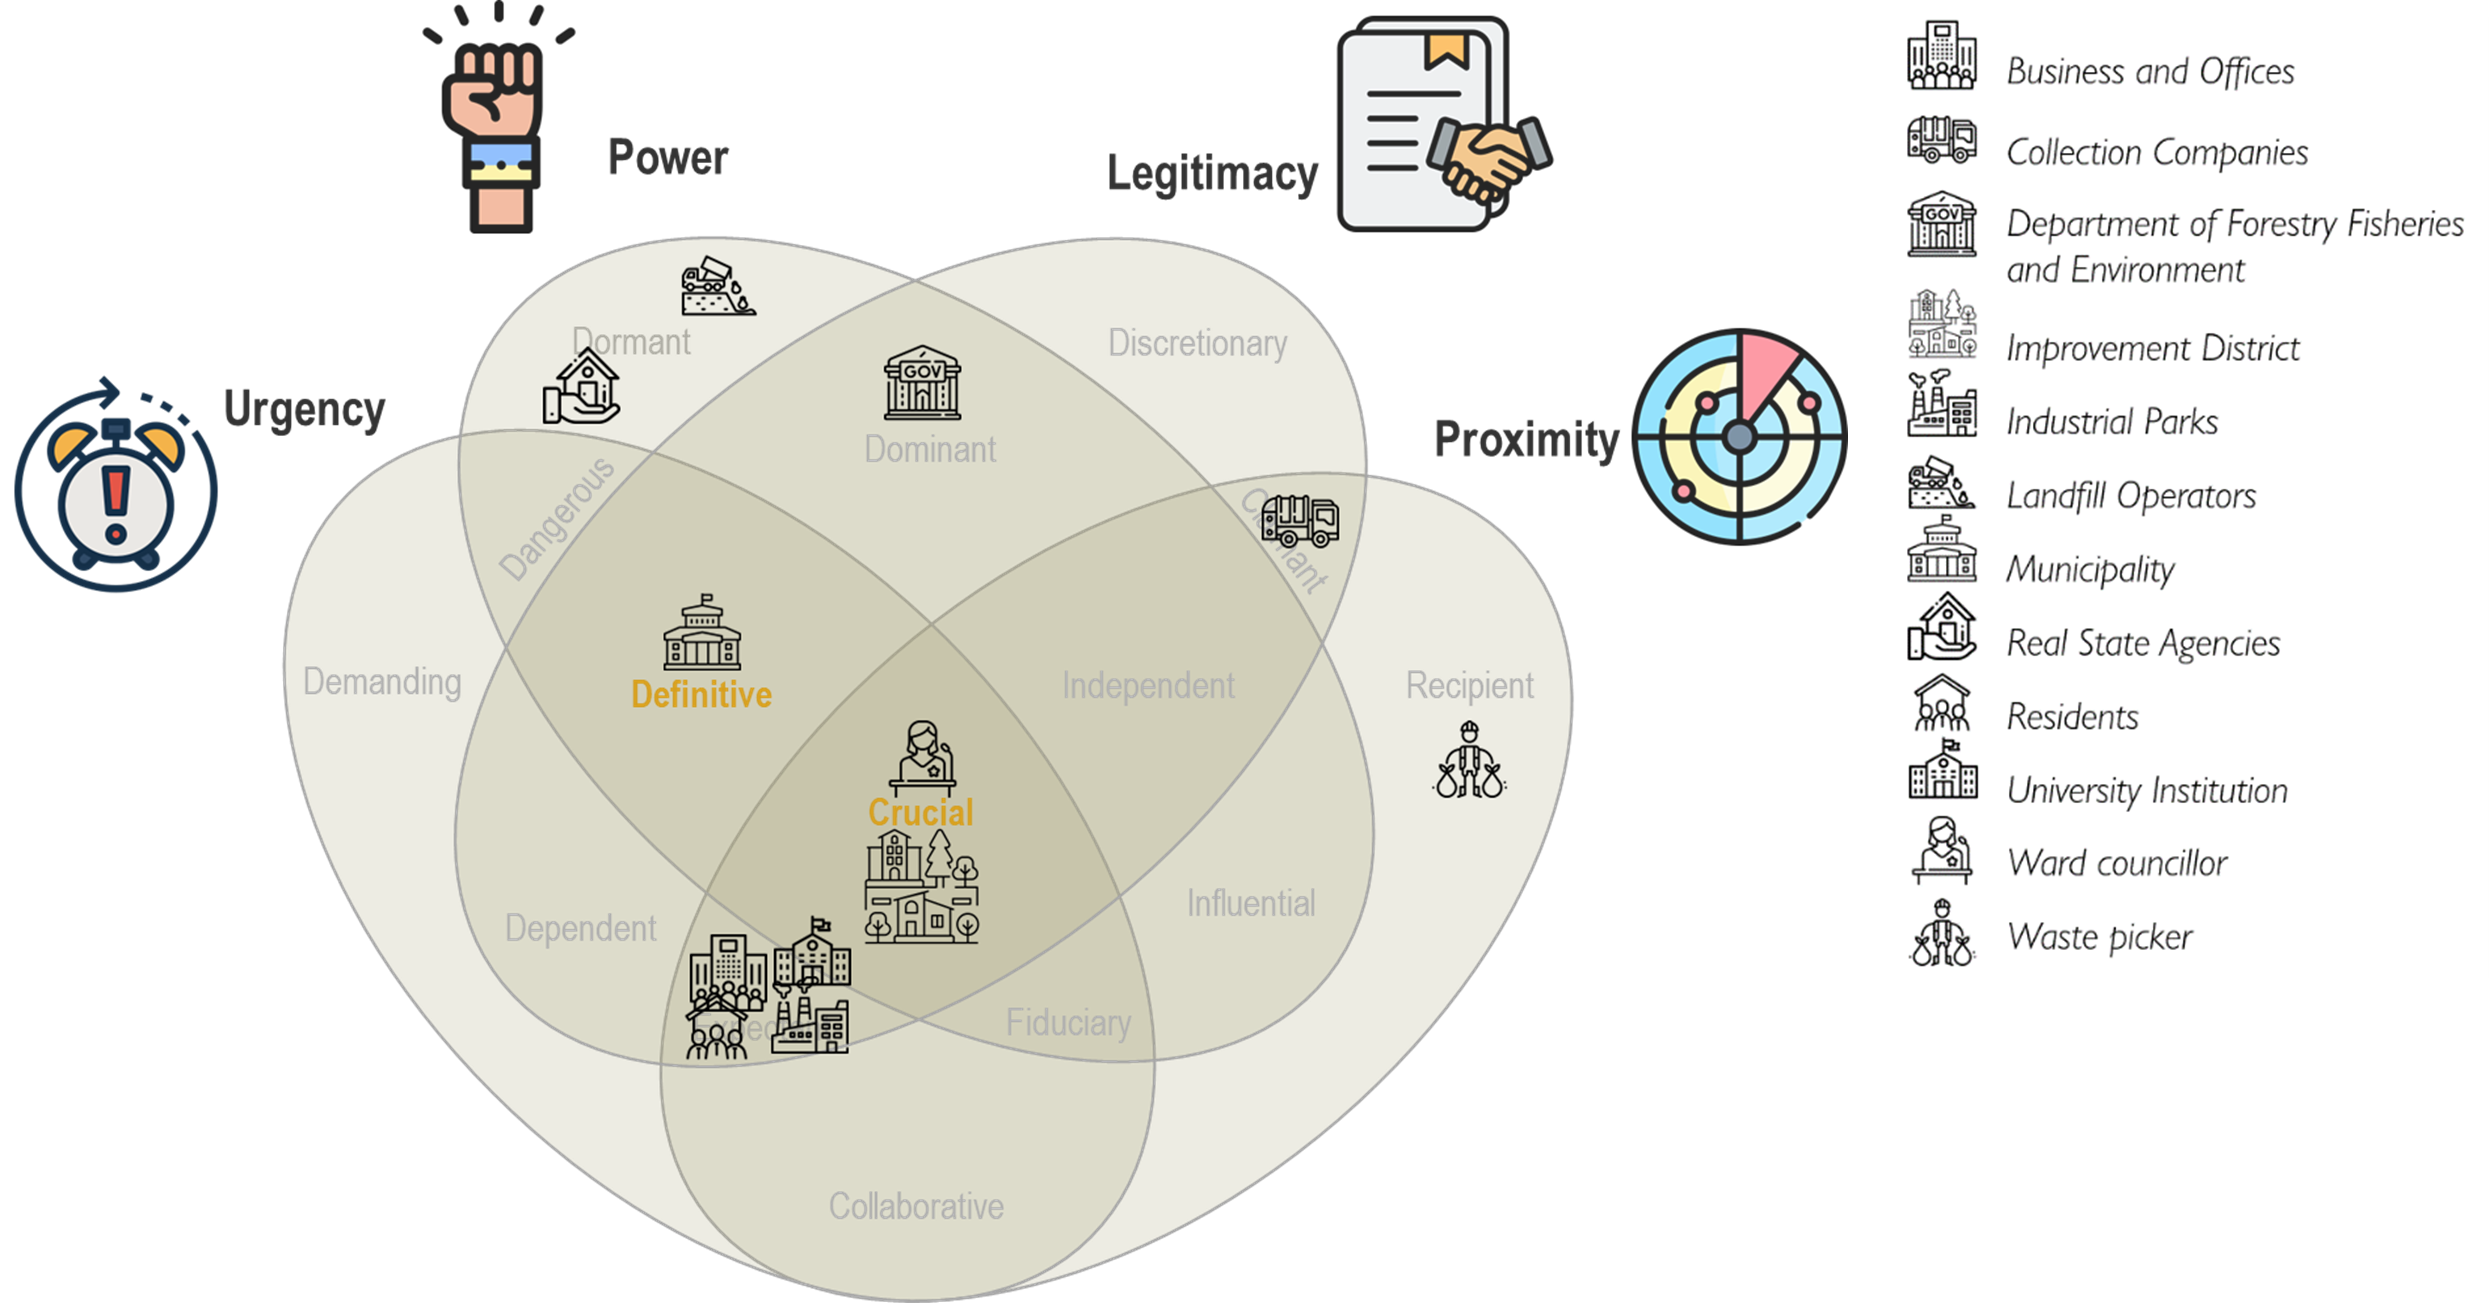
\includegraphics[width=1.2\linewidth]{Figures/Stakeholders map.png}
        \caption{Stakeholders’ typologies for Waste Collection Digital Twin.}
        \label{fig:typologies}
    \end{figure*}

    Stakeholders identified 32 requirements for improving SW management, with "zero waste" and "assessing environmental impact" being the most common. These can be grouped into Strategic, Performance, and Operational categories.% (Table \ref{tab:initialReq}). %The requirements emphasized the importance of aligning with the Sustainable Development Goals (SDGs), Nationally Determined Contributions (NDC) under the Paris Agreement, and European Sustainability Reporting (ESG) Standards (Table \ref{tab:initialReq}).
% \begin{center}
% \scriptsize
%     \begin{longtable}{l r}
%         \caption{Stakeholder user requirements} \label{tab:initialReq} \\
% %        \scriptsize
%         \toprule Category&Elements\\ \toprule \endfirsthead  
%         \toprule Category&Elements\\ \toprule \endhead  
%         \bottomrule 
%         \multicolumn{2}{r}{{Continued in next page}}\\ \midrule      \endfoot
%         \midrule 
%         \bottomrule \endlastfoot
%         \multirow{10}{*}{Strategic} &Carbon footprint reduction\\
%                                     &Environmental impact\\
%                                     &ESG reports\\
%                                     &Polluter Identification\\
%                                     &Reports to NDC for Paris Agreement\\
%                                     &Scalability to Country\\
%                                     &SDG Goals performance\\
%                                     &Sources of waste\\
%                                     &Type of waste generated\\
%                                     &Zero Waste\\
%         \midrule
%         \multirow{8}{*}{Performance}&Dedicated person-hours\\
%                                     &Optimally used container's location\\
%                                     &Recycling per building\\
%                                     &Recycling per campus (university)\\
%                                     &Recycling per sorting area\\
%                                     &Total Generation Waste\\
%                                     &Trucks Fuel consumption\\
%                                     &Waste production heatmaps\\
%         \midrule
%         \multirow{14}{*}{Operational}&Container capacity level\\
%                                     &Container location\\
%                                     &Data Time series\\
%                                     &Emissions measurement (odors)\\
%                                     &Event preparations\\
%                                     &Historic accumulation of waste\\
%                                     &Optimal collection route\\
%                                     &Proportion and quantities that go to landfill\\
%                                     &Real-time measurement\\
%                                     &Real-time generation\\
%                                     &Simple design\\
%                                     &Street sweepers distribution\\
%                                     &Visualization designed (also) for illiterate people\\
%                                     &Waste pickers distribution\\
%     \end{longtable}
% \end{center}
Considering the \textit{urgency} of \textit{definitive} and \textit{crucial} stakeholders and recognizing constraints (such as a short time frame, few resources, and external data beyond the methodology's scope), 17 identified requirements were excluded from the final UDT. Table \ref{tab:finalReq} lists the final included requirements.

    \begin{table}[h!]
        \centering
        \caption{Final Requirements included in the Waste Management Digital Twin.}
        \scriptsize
        \label{tab:finalReq}
        \begin{tabularx}{\linewidth}{X r}
            \toprule
            Category&Elements\\
            \midrule
            \multirow{5}{*}{Strategic}&Polluter Identification\\
                                        &Scalability to Country\\
                                        &SDG Goals performance (MSW Generated Tons/d)\\
                                        &Sources of waste\\
            \midrule
            \multirow{4}{*}{Performance}&Optimally used container's location\\
                                        &Total Generation Waste\\
                                        &Trucks Fuel consumption\\
                                        &Waste production heatmaps\\
            \midrule
            \multirow{6}{*}{Operational}&Container capacity level\\
                                        &Container location\\
                                        &Optimal collection route\\
                                        &Real-time generation\\
                                        &Simple design\\
                                        &Visualization designed (also) for illiterate people\\
            \bottomrule        
        \end{tabularx}
    \end{table}

 %    \subsection{Building reconstruction and identification} \label{subsec:buildingsRes}
 %    The proposed method extracted footprints from 4,768 buildings (see section \ref{subsubsec:Buildings}). The accuracy, based on a random 1,000-point allocation, is presented in Table \ref{tab:confMatrix}. After visual inspection, 663 polygons were removed, corresponding to trees, cars, car shades, and bushes. Students validated 424 buildings  (10.33\%) in residential areas. After validation and visual inspection of aerial imagery, along with OSM data, 123 buildings were not classified. The distribution of buildings per class is presented in Figure \ref{fig:corroboration}, where "Function" refers to parking lots, sheds, and garages. Following attribute correction and extraction, the buildings were transformed into a 3D multipatch, as depicted in Figure \ref{fig:3Drepr1}.

 %    \begin{table*}[h!]
 %        \caption{Confusion Matrix Building Identification}
 %        \label{tab:confMatrix}
 %        \scriptsize
 %        \begin{tabularx}{\linewidth}{XXXXX}
 %        \toprule
 %                                                        &                          & \multicolumn{3}{c}{Calculated State} \\ \midrule
 %        \multicolumn{1}{l|}{}                              &                          & Building   & Non-Building   & TOTAL  \\
 %        \multicolumn{1}{c|}{\multirow{3}{*}{Actual State}} & Building                 & 119        & 34             & 153    \\
 %        \multicolumn{1}{c|}{}                              & Non-Building             & 14         & 833            & 847    \\
 %        \multicolumn{1}{c|}{}                              & Total                    & 133        & 867            & 1000   \\ \midrule
 %                                                        & Positive Predicted Value &            &                & 0.895  \\
 %                                                        & False Omission Rate      &            &                & 0.039  \\
 %                                                        & Accuracy                 &            &                & 0.986  \\ \bottomrule
 %        \end{tabularx}
 %    \end{table*}

 % \begin{figure}[H]
 %    \centering
 %    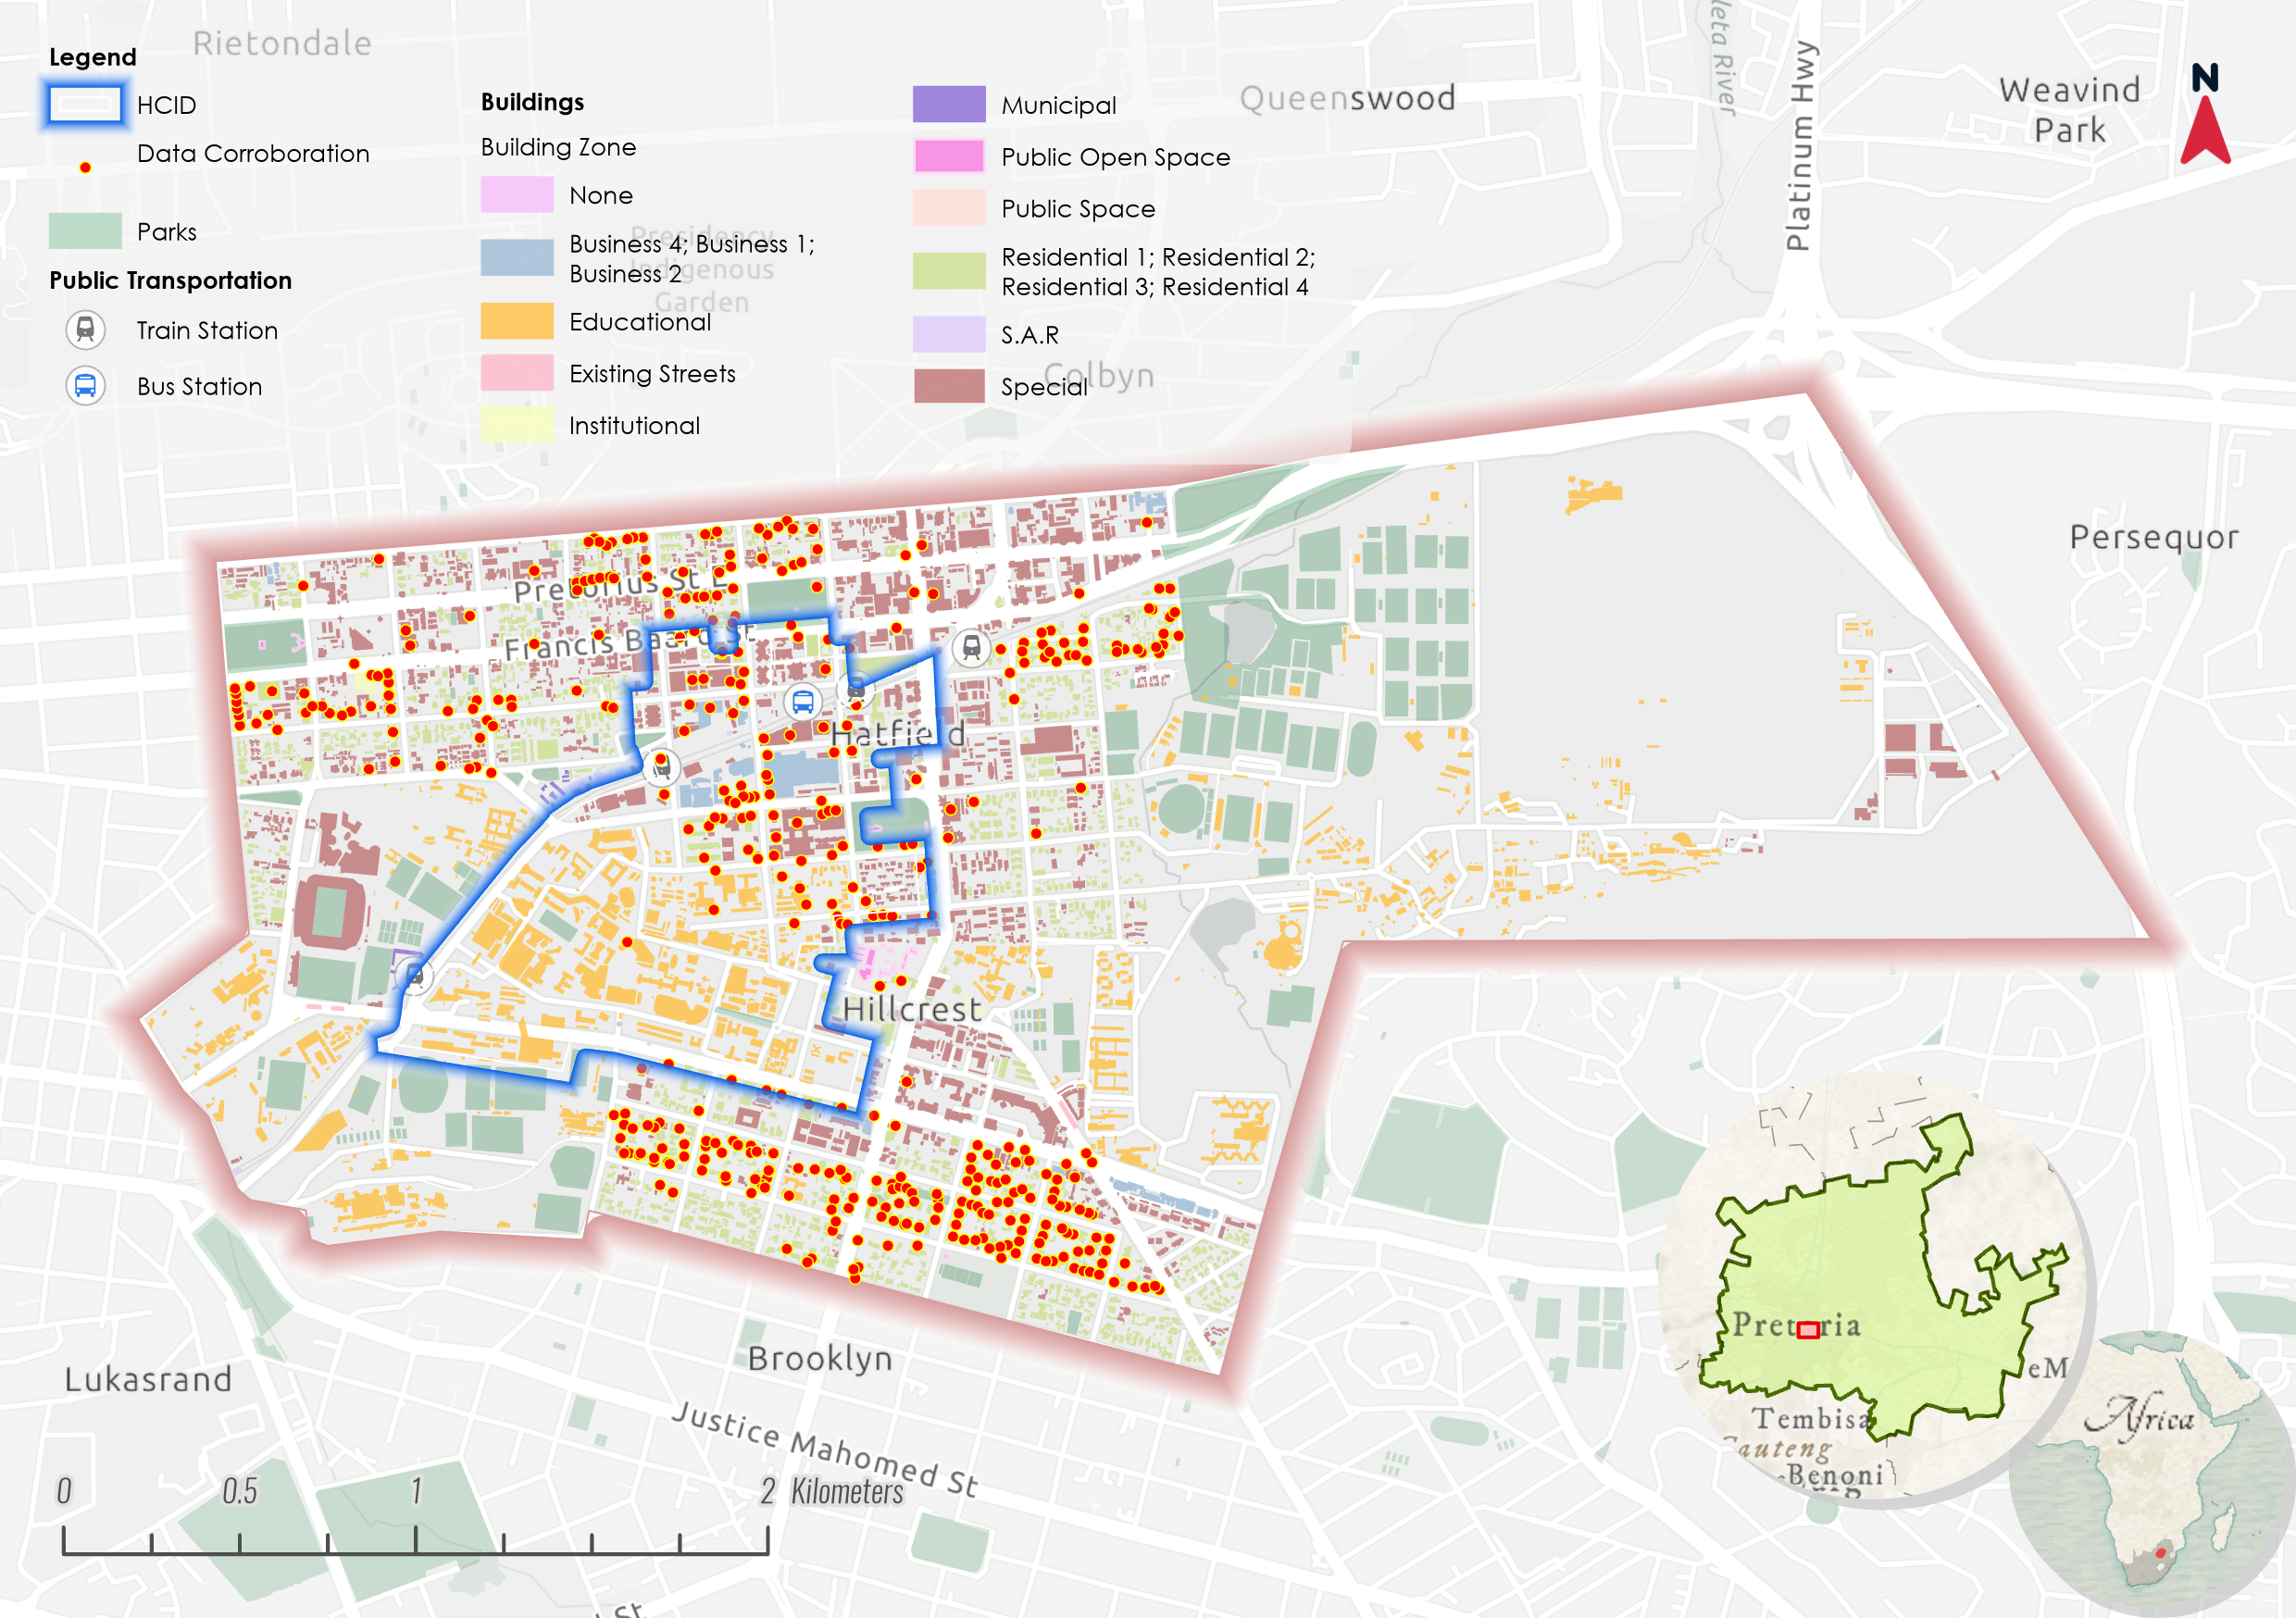
\includegraphics[width=0.8\linewidth]{Figures/Data Corroboration.png}
 %        \caption{Data corroboration on building attributes}
 %        \label{fig:corroboration}
 %    \end{figure}
    
 %    \begin{figure}[H]
 %    \centering
 %    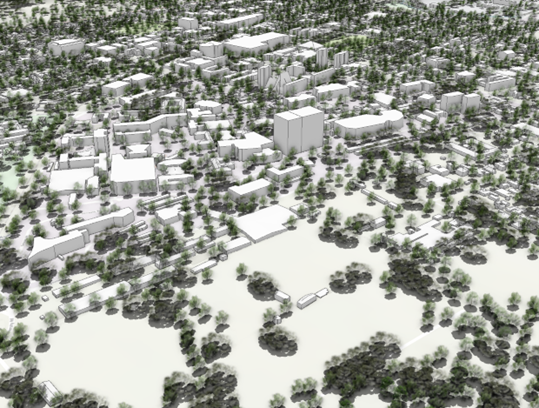
\includegraphics[width=0.8\linewidth]{Figures/3D Study Area.png}
 %        \caption{Study Area 3D Representation. Trees were extracted from LIDAR Scanning}
 %        \label{fig:3Drepr1}
 %    \end{figure}

 %    The building footprint area ranges from 3.5 m$^2$ (a small yet tall maintenance structure) to 25,885 m$^2$ (Loftus Stadium), where 3,506 buildings (85.4\%) do not exceed 500 m$^2$. Figure \ref{fig:buildfoot} shows consistent area distribution per building class, with few outliers. The aggregated footprint extent of the study area is 1,433,951.96 m$^2$, with habitational and school classes occupying more surface land. %(Figure \ref{fig:buildAgg}).

 %    \begin{figure}[ht]
 %    \centering
 %    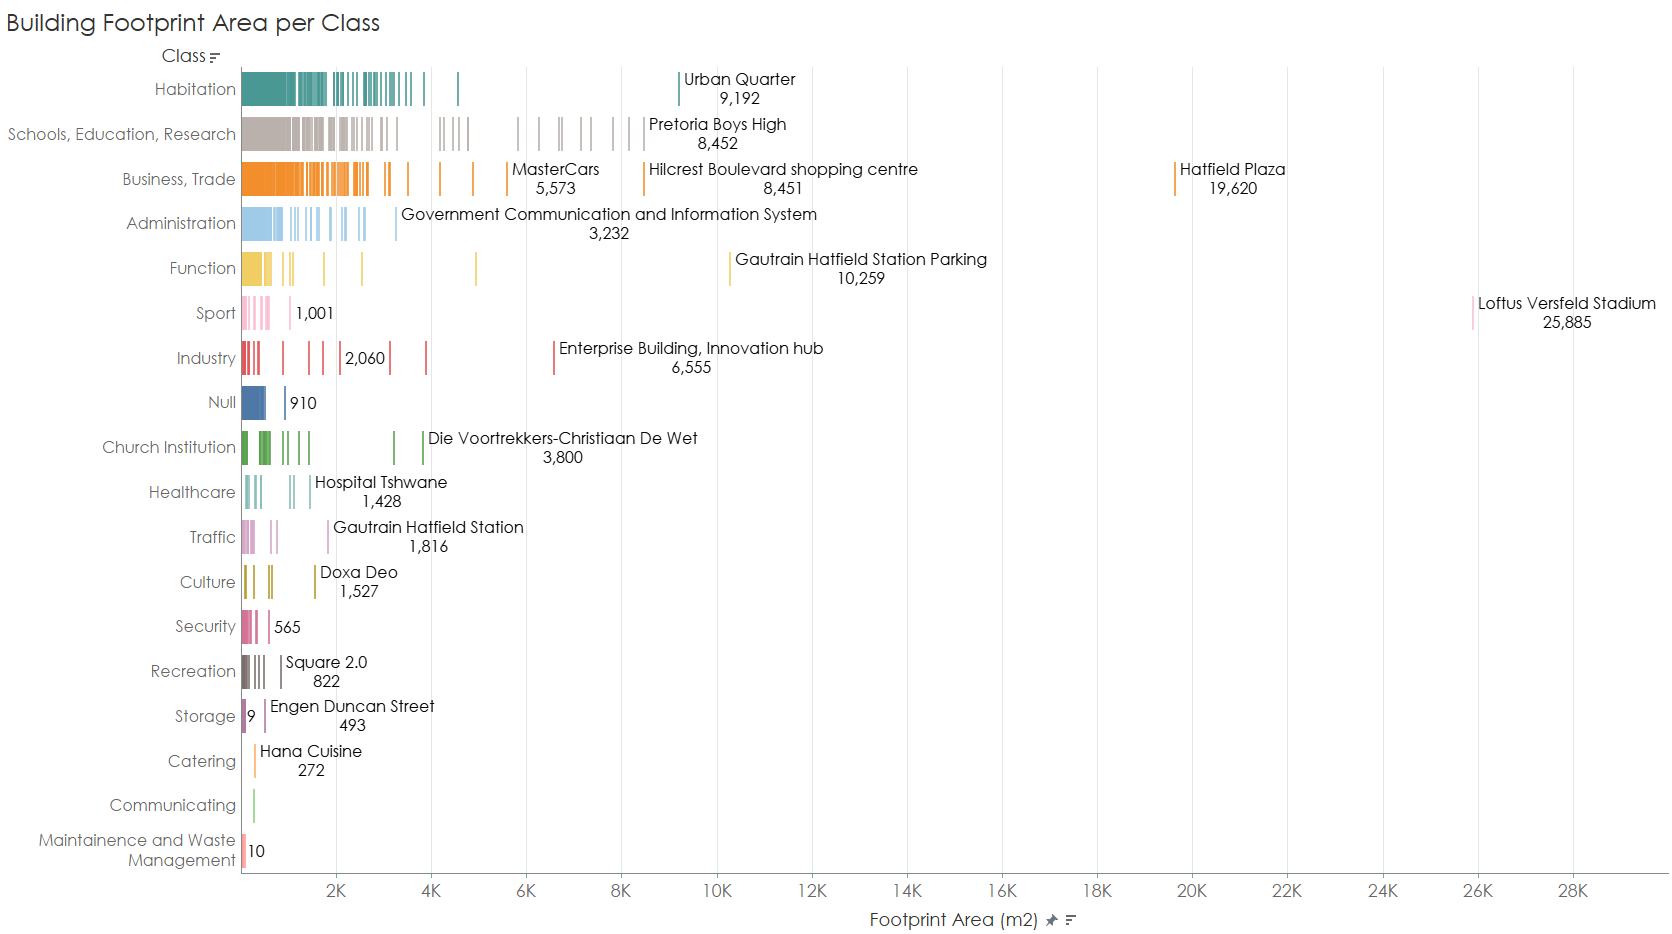
\includegraphics[width=\linewidth]{Figures/Bulding Area.png}
 %       \caption{Building Footprint Area per building Class. For each class, the largest building and its area are shown.}
 %       \label{fig:buildfoot}
 %    \end{figure}

 %    % \begin{figure*}[htb]
 %    % \centering
 %    % 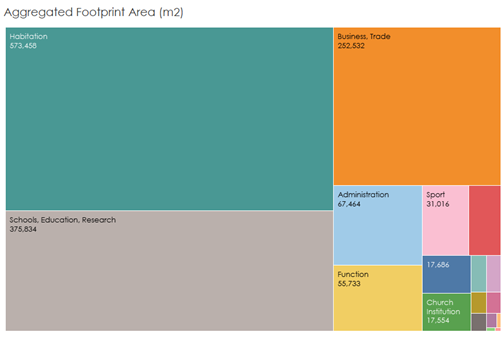
\includegraphics[width=0.8\linewidth]{Figures/FootprintArea.png}
 %    %     \caption{Aggregated Footprint Area distribution per building Class}
 %    %     \label{fig:buildAgg}
 %    % \end{figure*}

 %    Figure \ref{fig:areaMap} displays the distribution of total footprint area, ranging from 7m$^2$ (a security booth) to 336,510.36 m$^2$ (Loftus Stadium). Larger floor area buildings are mainly located in the Hatfield CID. The aggregated footprint extent of the study area is 5,681,494.72 m$^2$, with habitational and school classes also, occupying the most extensive total floor area. The "function" buildings occupy a significant portion of the overall area, with administrative buildings ranking sixth in the total occupied area. This is attributed to the city's significant car dependency and multiple floors of parking lots, excluding underground parking.

 %    \begin{figure}[ht]
 %    \centering
 %    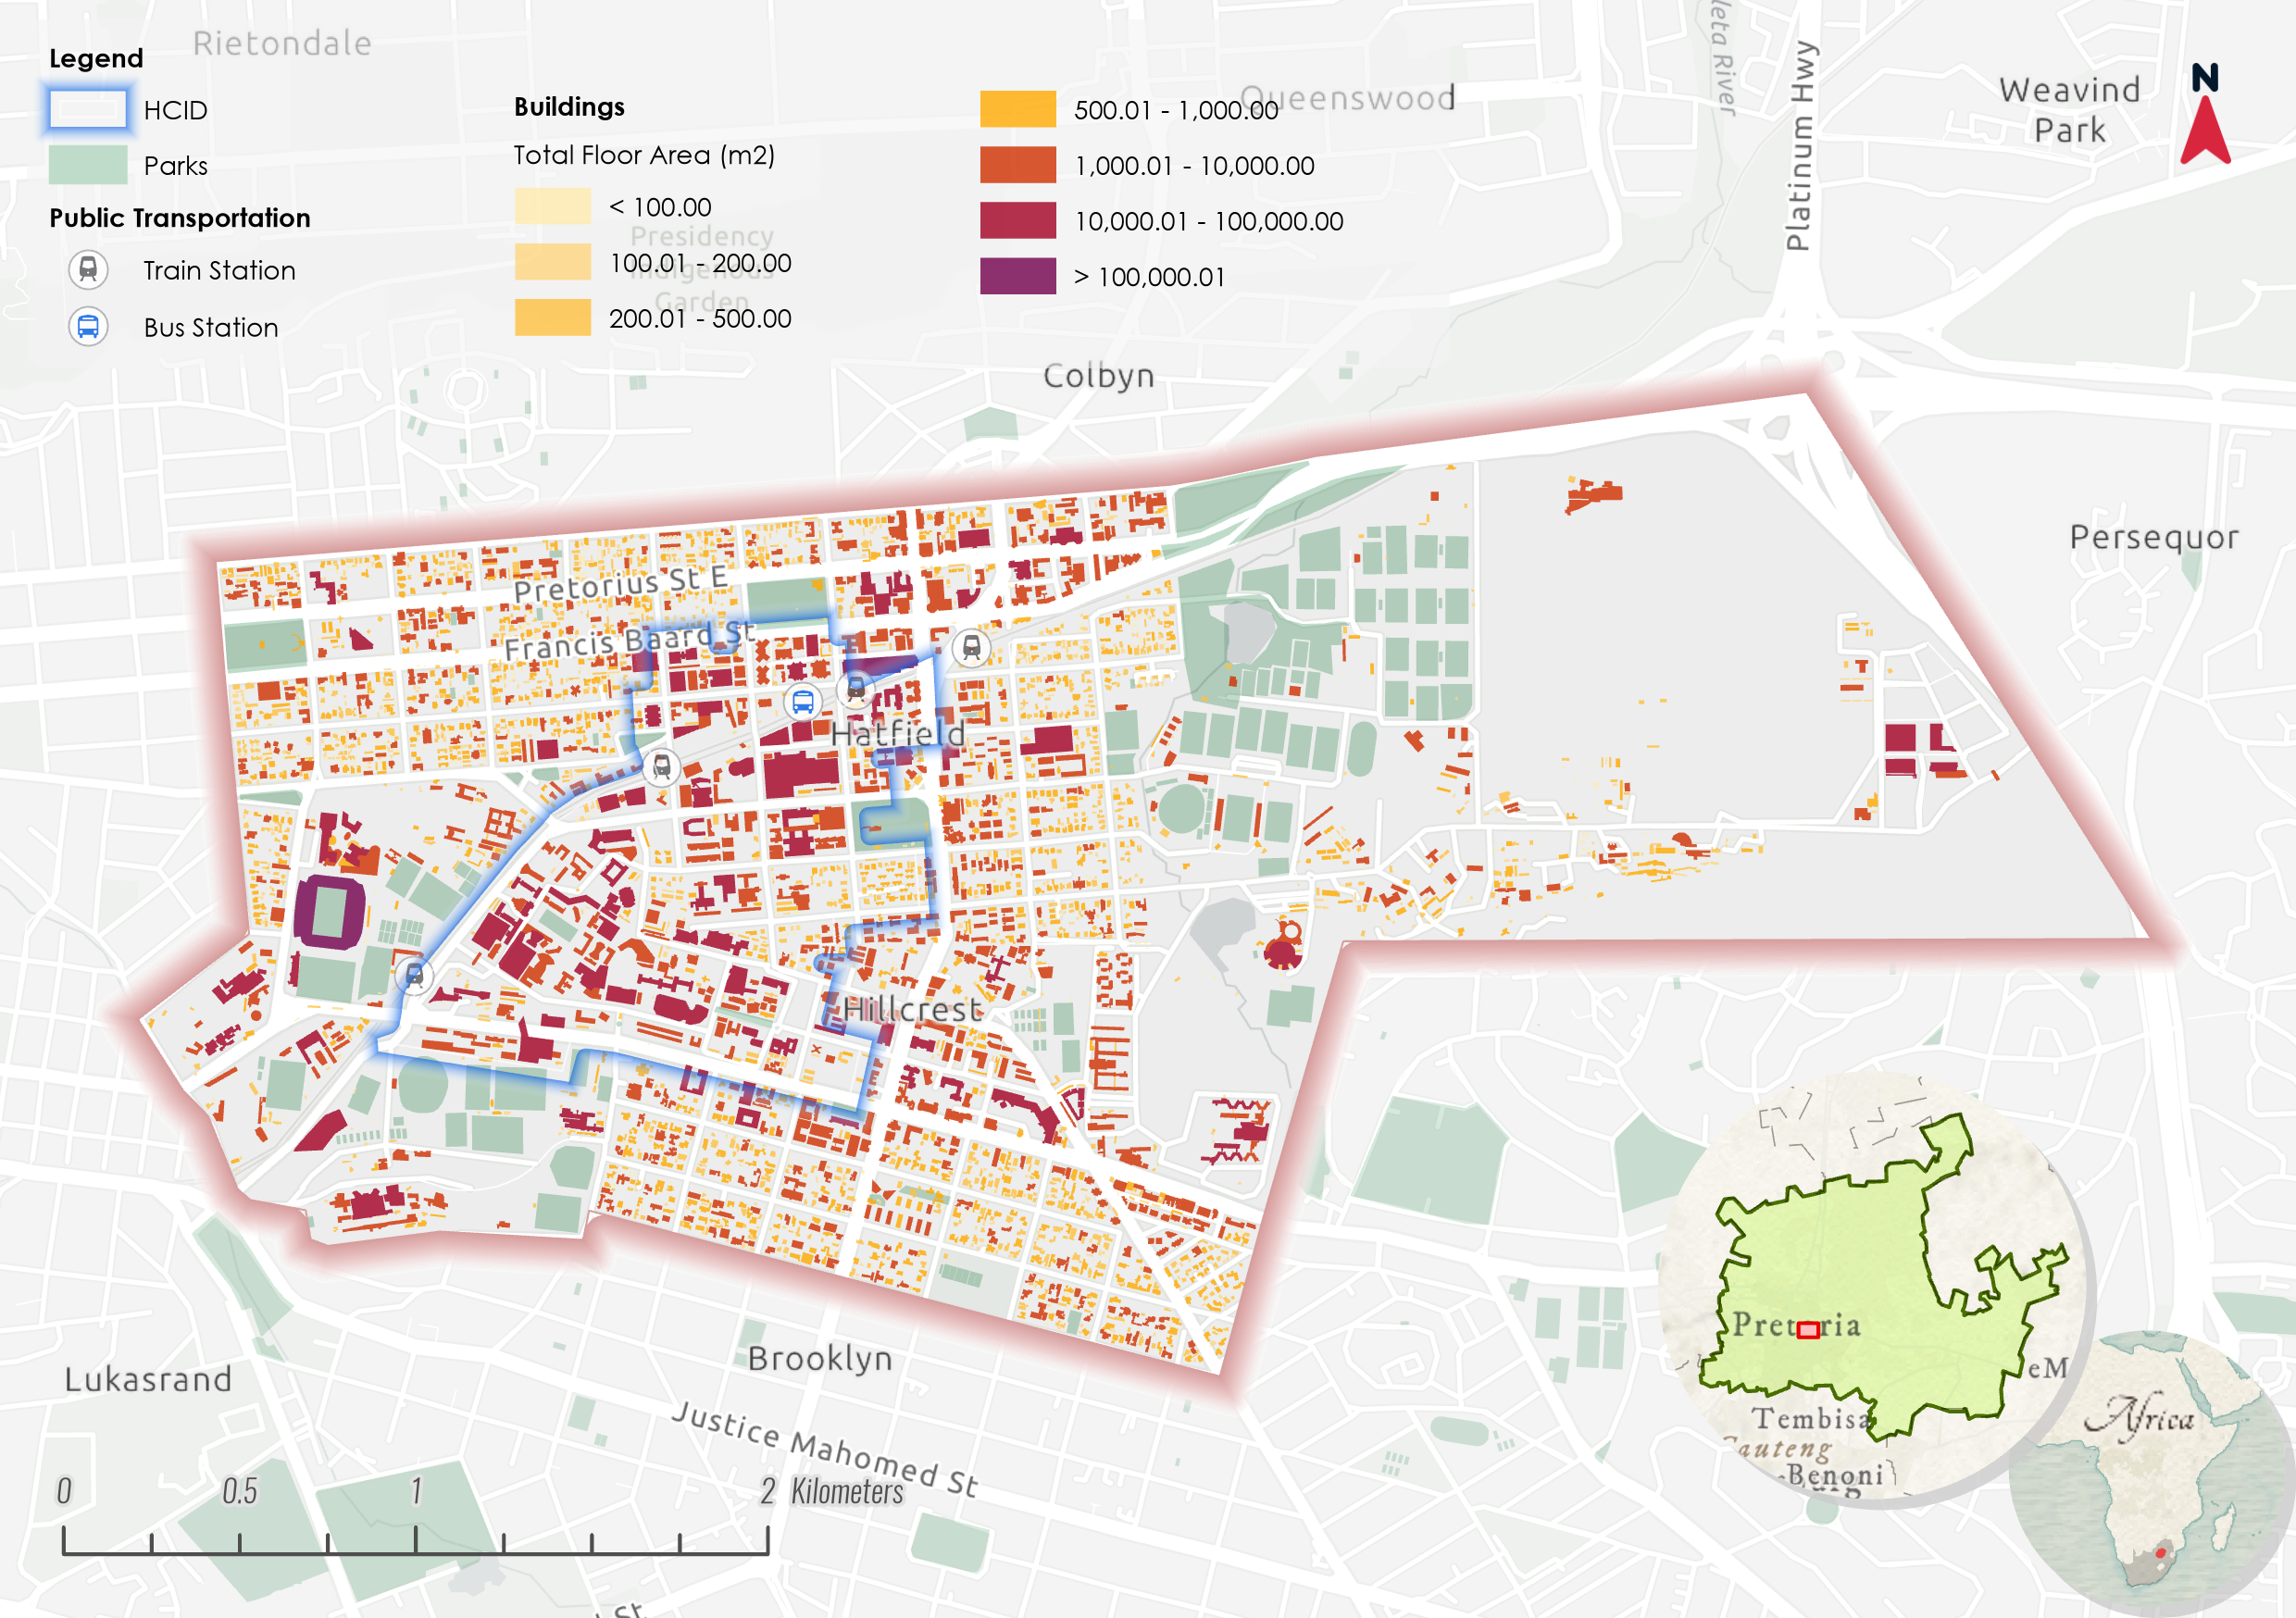
\includegraphics[width=0.9\linewidth]{Figures/Building Total Floor Area.png}
 %        \caption{Buildings Total Floor Area ($m^2$)}
 %        \label{fig:areaMap}
 %    \end{figure}

    \subsection{Solid waste generation analysis} \label{subsec:SolidWasteGen}
   Buildings were assigned to the closest container (Figure \ref{fig:closestCont}). The maximum distance assigned is 881.80 m, equivalent to a 14-minute walk (calculated at 1m/s walking speed). This distance applies to buildings in the industrial park (east of the study area), which were inaccessible during data collection. It's possible that closer containers exist or each building has its own container within manufacturing facilities. Excluding industrial buildings, the longest assignment distance is 427.40m, equivalent to a 7.1-minute walk. The average distance from a building to a container is 90.55m. For non-residential buildings, the average distance is 86.08m, with a median of 72.51m and a standard deviation of 58.16m. The minimum distance from a building to a container is 2.51m. Figure \ref{fig:distances} illustrates the distribution of calculated distances for all buildings.

    \begin{figure*}[!ht]
    \centering
    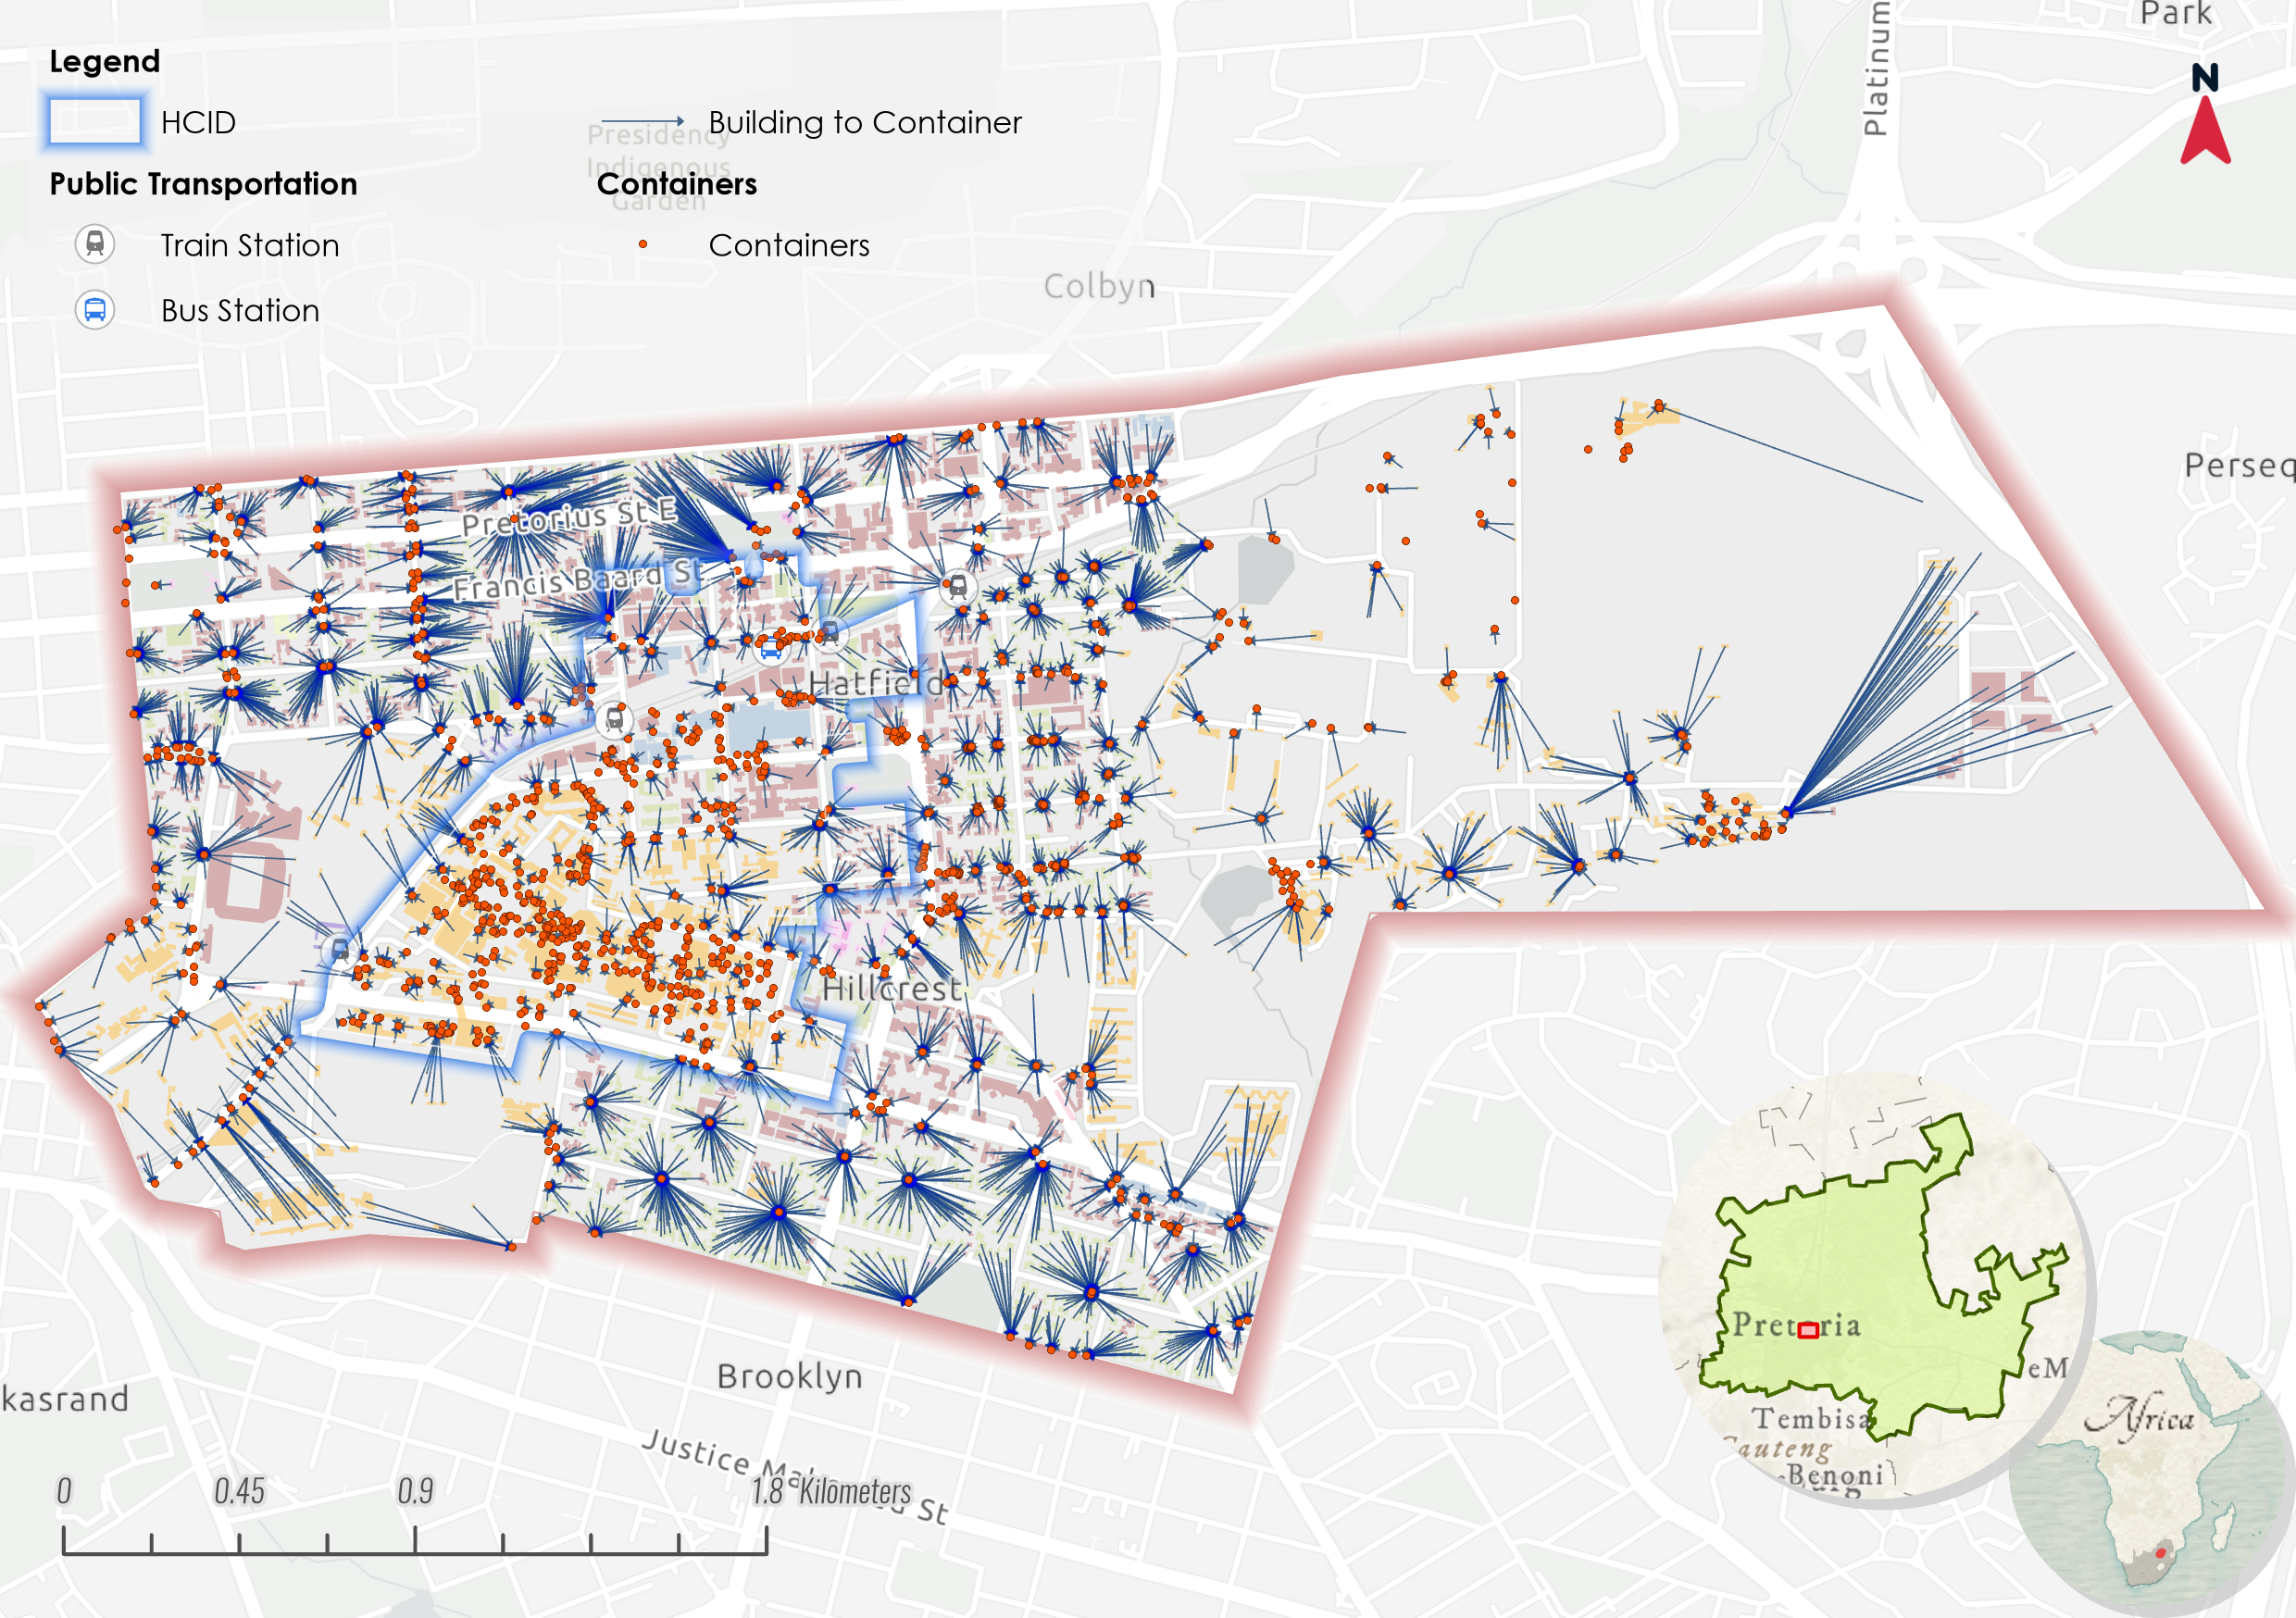
\includegraphics[width=1.2\linewidth]{Figures/Building to Container.png}
        \caption{Building to Container Assignation map.}
        \label{fig:closestCont}
    \end{figure*}

    \begin{figure*}[h!]
    \centering
        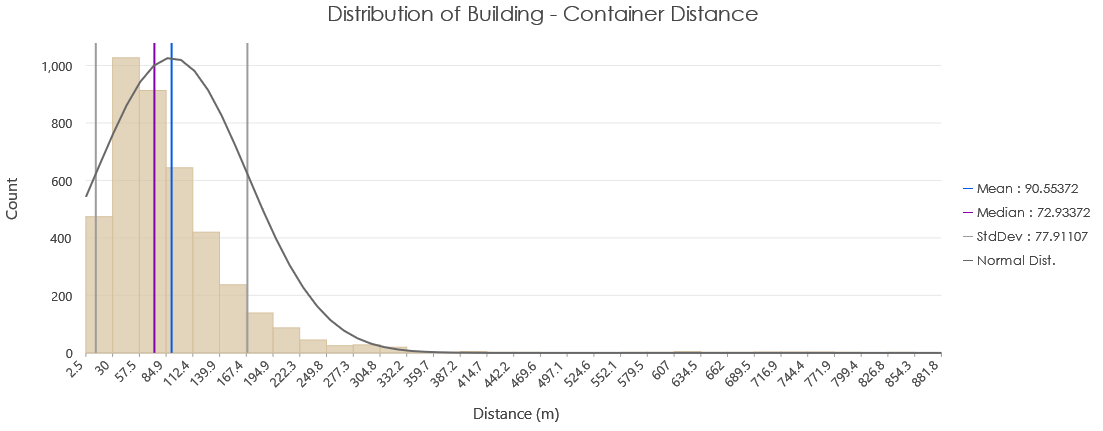
\includegraphics[width=\linewidth]{Figures/Building to container distance.png}
        \caption{Distribution of Building to Container distances in meters.}
        \label{fig:distances}
    \end{figure*}

    Based on average production per capita, residential buildings' waste production ranges from 0 kg/d to 1,575.60 kg/d, with an average of 11.19 kg/d. Due to the method used to calculate inhabitants per building and low population density on each 100x100m grid, 662 buildings (31.95\%) have no residents and, therefore, no waste production. Despite this gap in waste estimation, calculated values for residential buildings total 23.12 tons of waste produced daily.

    For non-residential buildings, Category D has the highest number of buildings (see Figure \ref{fig:buildWaste} and Table \ref{tab:Waste2}). The largest waste production is in Category C, which includes the sports stadium, with a total estimated SW production of 251.81 tons per day \footnote{Due to the sports stadium's event-based operation and high waste production, it was excluded from the daily optimal route calculation. The absence of a designated container for this building, along with its large waste volume, may lead to errors. Placing containers inside rather than in public areas could lead to trucks focusing solely on collecting this waste, deviating from the normal waste collection routine in the city.}. Category A, with only 73 buildings, has a waste production estimate totaling 149.83 tons daily.

    According to estimate calculations, the largest waste producers are educational buildings, generating 198.51 tons/day (42.64\%), and Business and Commercial buildings, producing 170 tons/day (36.58\%). Overall, the largest waste producers include the Sports Stadium (Estimate: 41.72 tons/day), two shopping centers (41.10 and 17.71 tons/day, respectively), and the Information Technology Building of UP (8.08 tons/day).
    
    \begin{figure*}[ht]
    \centering
    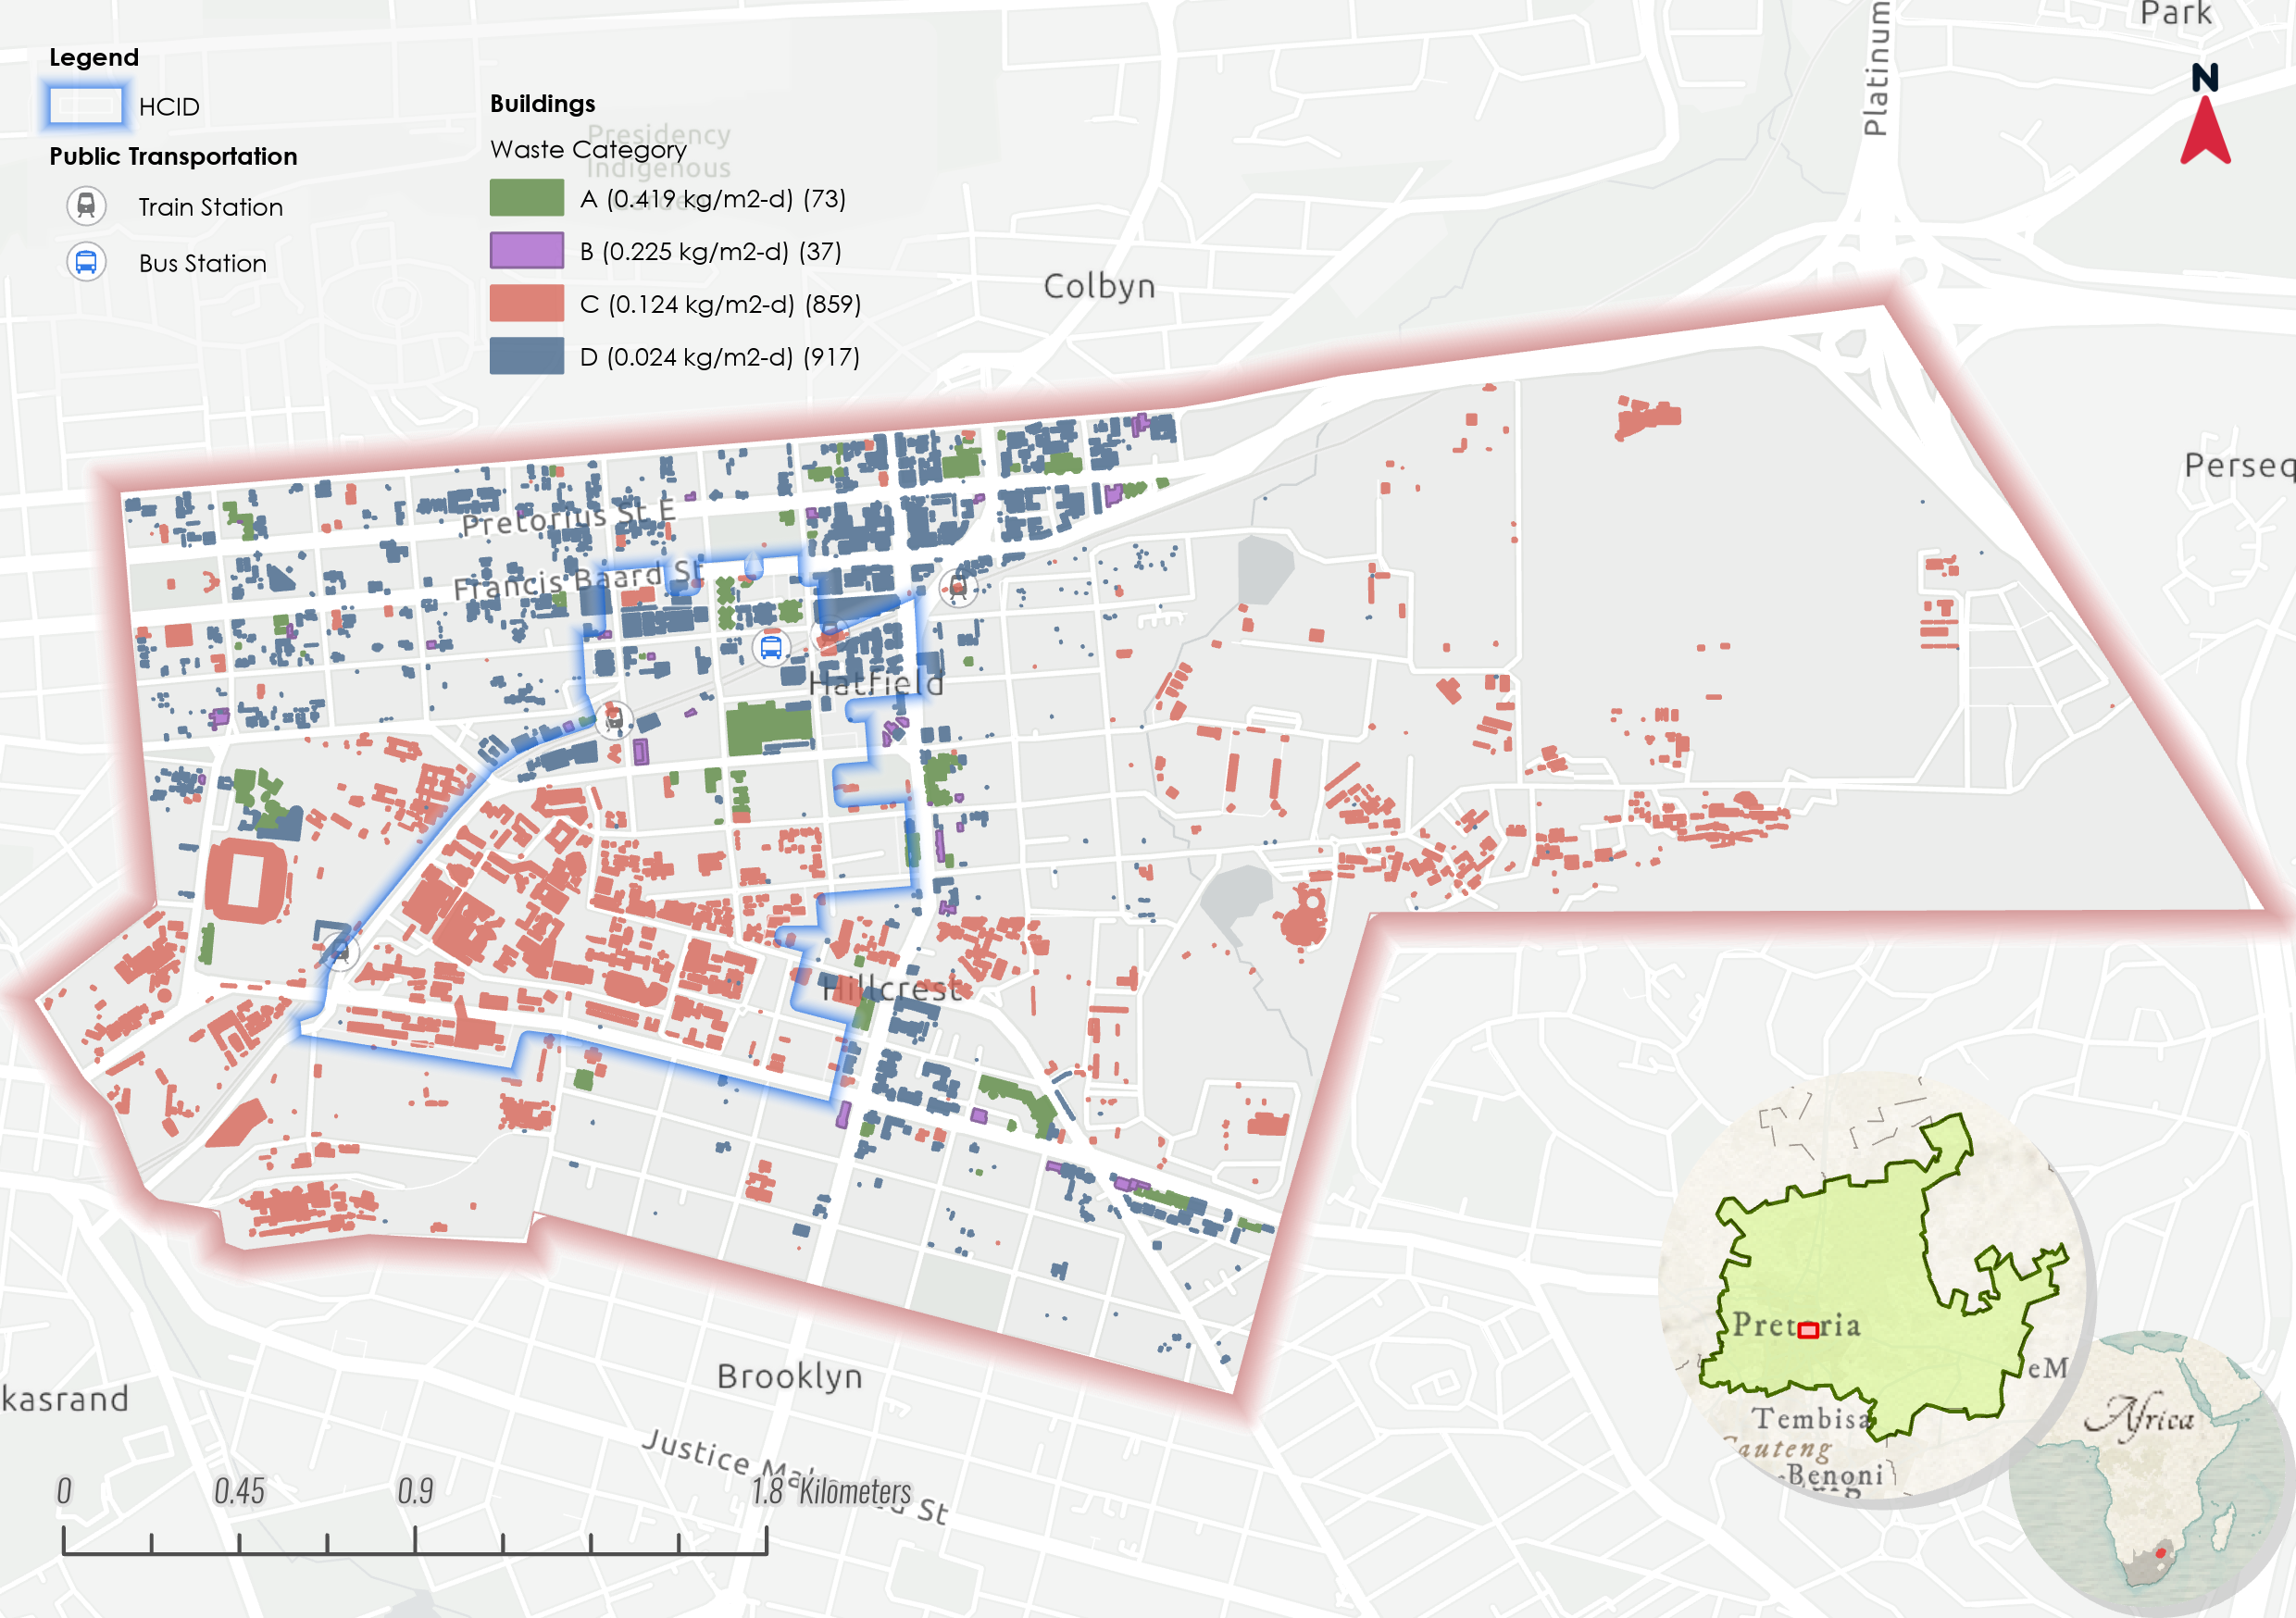
\includegraphics[width=1.2\linewidth]{Figures/Waste Categories.png}
        \caption{Building Classification per Waste Category}
        \label{fig:buildWaste}
    \end{figure*}

    \begin{table}[!h]
        \centering
        \caption{Estimate waste production per building category}
        \scriptsize
        \label{tab:Waste2}
        \begin{tabularx}{\linewidth}{l LLLLL}
            \toprule
            Building Category&Total Waste Production (kg/d)&MAX per building (kg/d)&MIN per building (kg/d)&Average (kg/d)& Std. Dev\\ 
            \midrule
            A&149,828.77&41,103.38&27.72&2,052.45&5,301.89\\
            B&14,169.03&1,531.37&5.00&382.95&425.22\\
            C&251,811.20&41,727.28&1.16&293.14&1,578.39\\
            D&26,581.51&2,462.11&0.17&28.99&106.64\\
            \midrule
            TOTAL&442,390.52&41,727.28&0.17&234.57&1,538.57\\
            \bottomrule
        \end{tabularx}
    \end{table}

    \subsection{Hourly Solid Waste Generation Simulation} \label{subsec:Simulation}

    Considering this production and simulating hourly waste generation from each building, simulations illustrate the status of containers at every hour before calculating the optimal collection route (Figure \ref{fig:Sim1}). These simulations demonstrate that 18 containers are saturated at the beginning of simulated hour 1, indicating sub-optimal use and showing a need for higher capacity allocation. By simulated hour 6, when containers are set for collection, there are 116 bins with a total volume of 56.5 tons. Waste generation is simulated randomly, leading to varying values and locations across simulations. However, areas near the stadium, within the university campus, and near the train station stops consistently require frequent collection to prevent container overflow.

    \begin{figure}[h!]
        \centering
        \begin{subfigure}[b]{0.45\linewidth}
        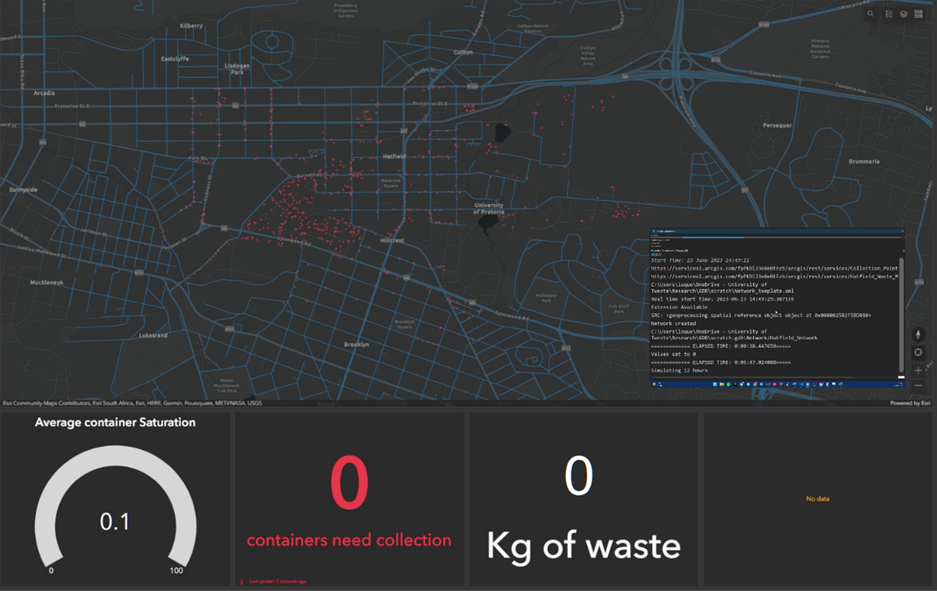
\includegraphics[width=\linewidth]{Figures/Sim1.png} 
        \caption{Initial State}
    \end{subfigure}
    \begin{subfigure}[b]{0.45\linewidth}
        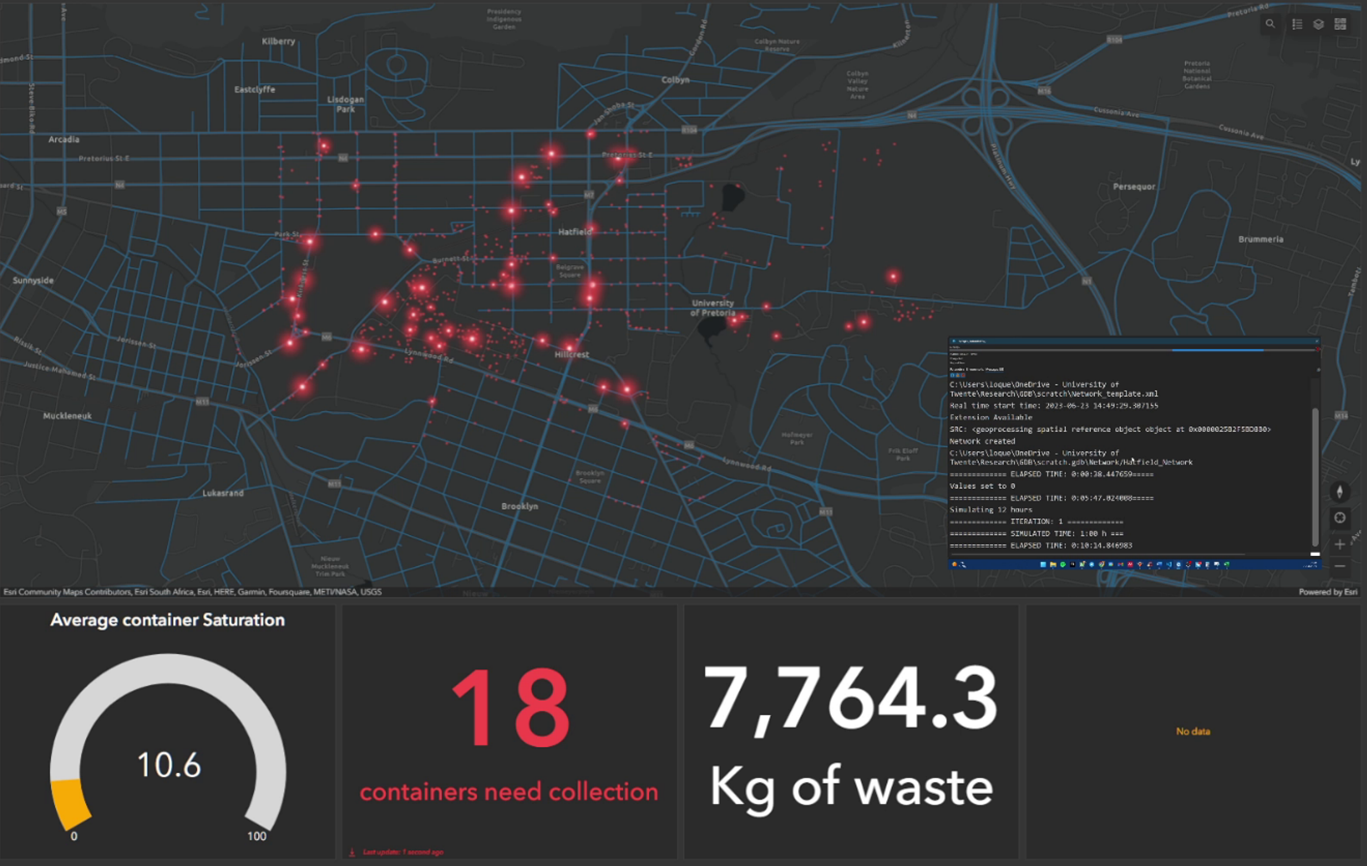
\includegraphics[width=\linewidth]{Figures/Sim2.png}
        \caption{Hour 1}
    \end{subfigure}
    \begin{subfigure}[b]{0.45\linewidth}
        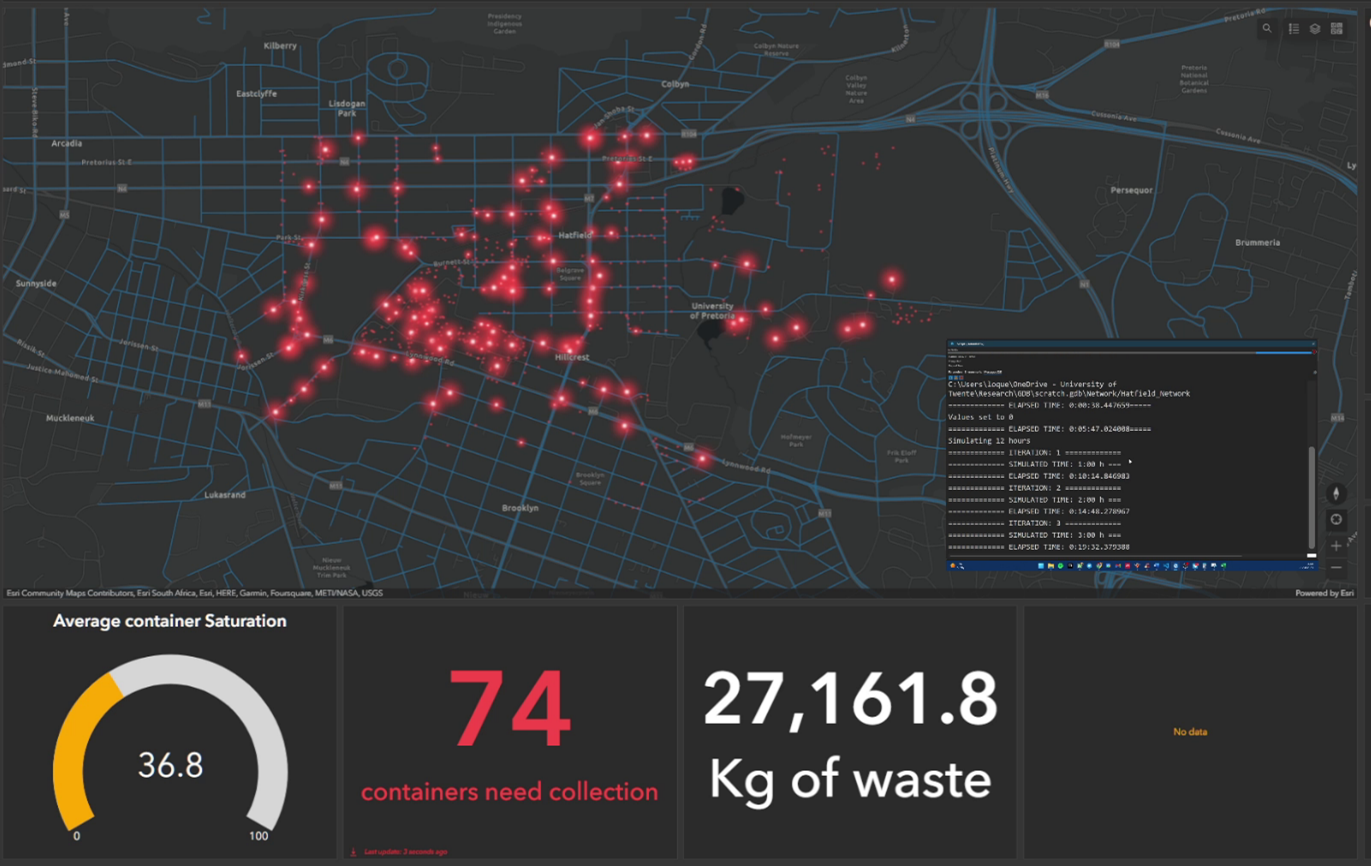
\includegraphics[width=\linewidth]{Figures/Sim3.png}
        \caption{Hour 3}
    \end{subfigure}
    \begin{subfigure}[b]{0.45\linewidth}
        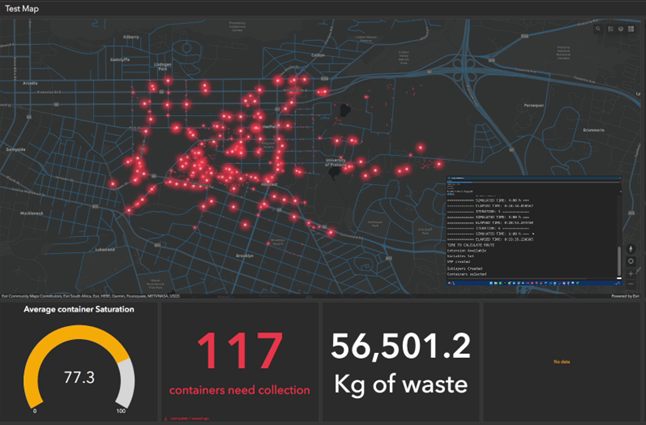
\includegraphics[width=\linewidth]{Figures/Sim6.png}
        \caption{Hour 6 - step before route calculation.}
    \end{subfigure}
    \caption{Waste Generation Simulation}
        \label{fig:Sim1}
    \end{figure}

    \subsection{Optimal Collection Routes}\label{subs:Optimalroute}
    
    The analyzed road network comprises 2,792 edges with speeds ranging from 40 km/h in residential areas to 120 km/h on . %(see Figure \ref{fig:road1}). 
   % Segment lengths vary from 9 cm (dangling arc error) to 2.97 km, with a median of 160.39 m and a standard deviation of 239.56 m. Time (weight) on these edges ranges from 0.25 ms (9cm segment) to 2.97 min, with a standard deviation of 12.92 seconds. 
   A total of 1,572 edges (56.30\%) were identified as unidirectional, mainly located within the study area and corresponding to local roads, while peripheral highways and arterial roads are bidirectional.% (Figure \ref{fig:road2}).

    % \begin{figure*}[h!]
    % \centering
    % 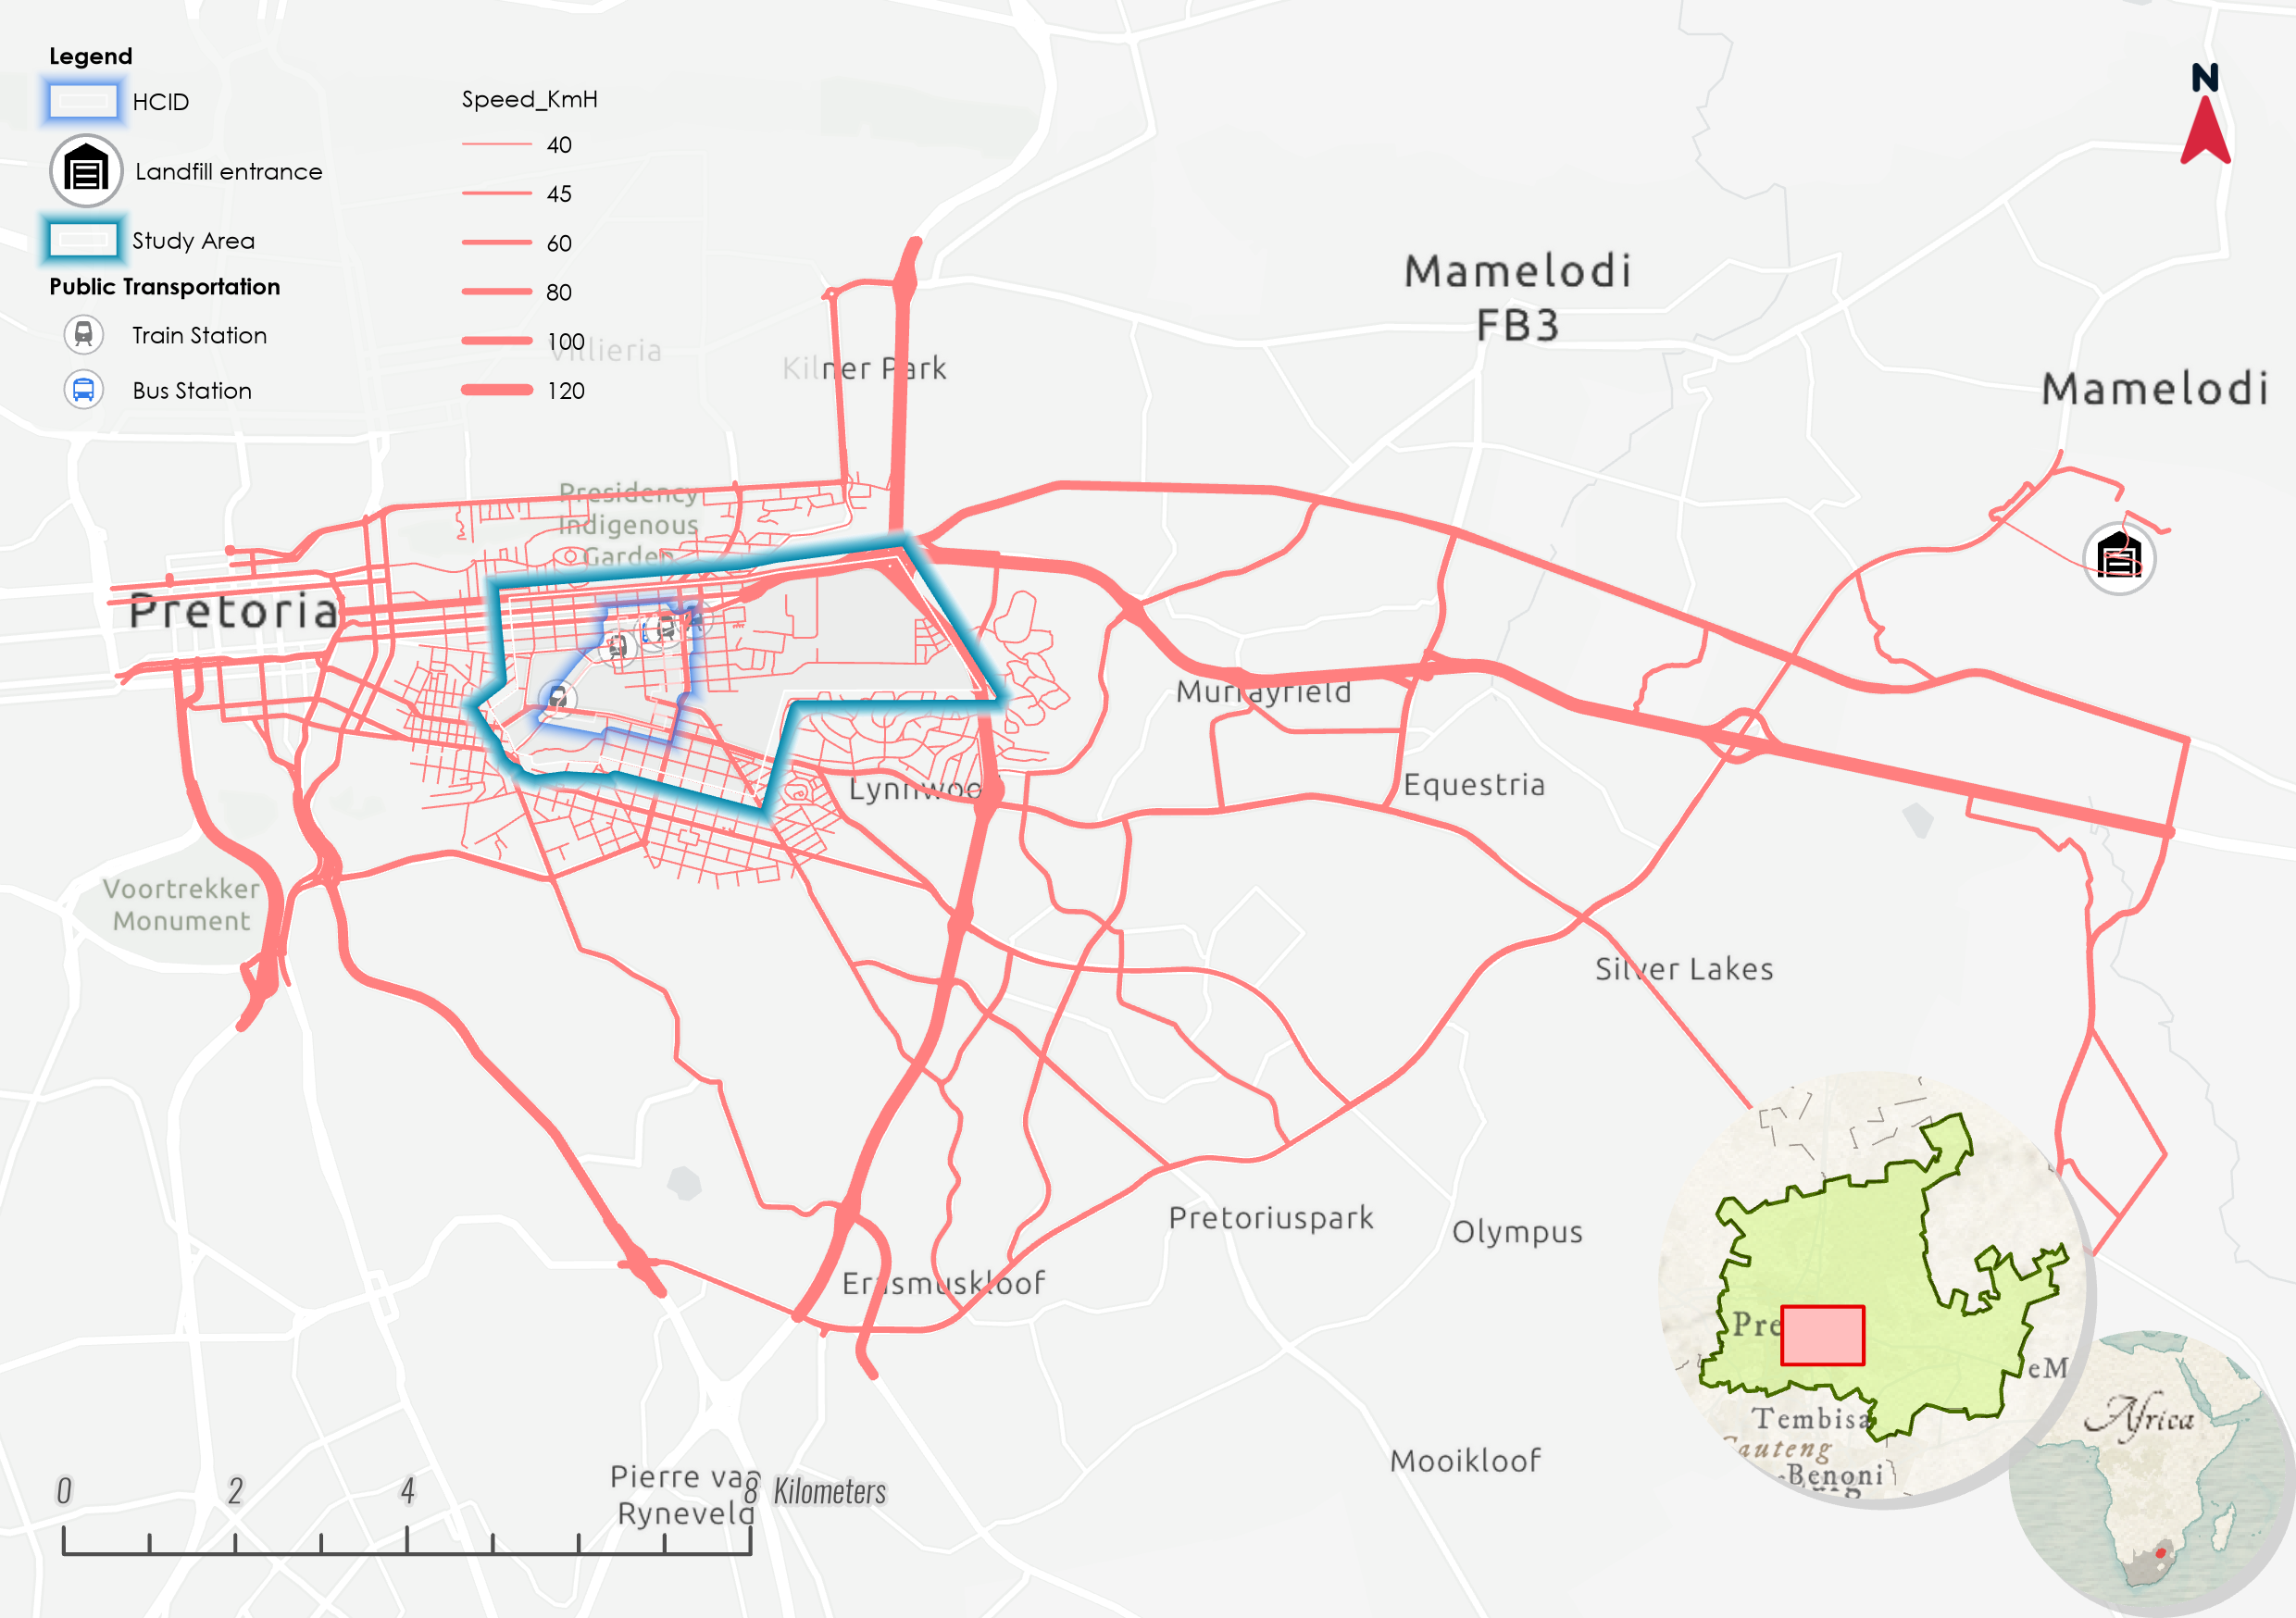
\includegraphics[width=0.85\linewidth]{Figures/Road Speed.png}
    %     \caption{Roads speed from Landfill to Study Area}
    %     \label{fig:road1}
    % \end{figure*}

    % \begin{figure*}[h!]
    % \centering
    % 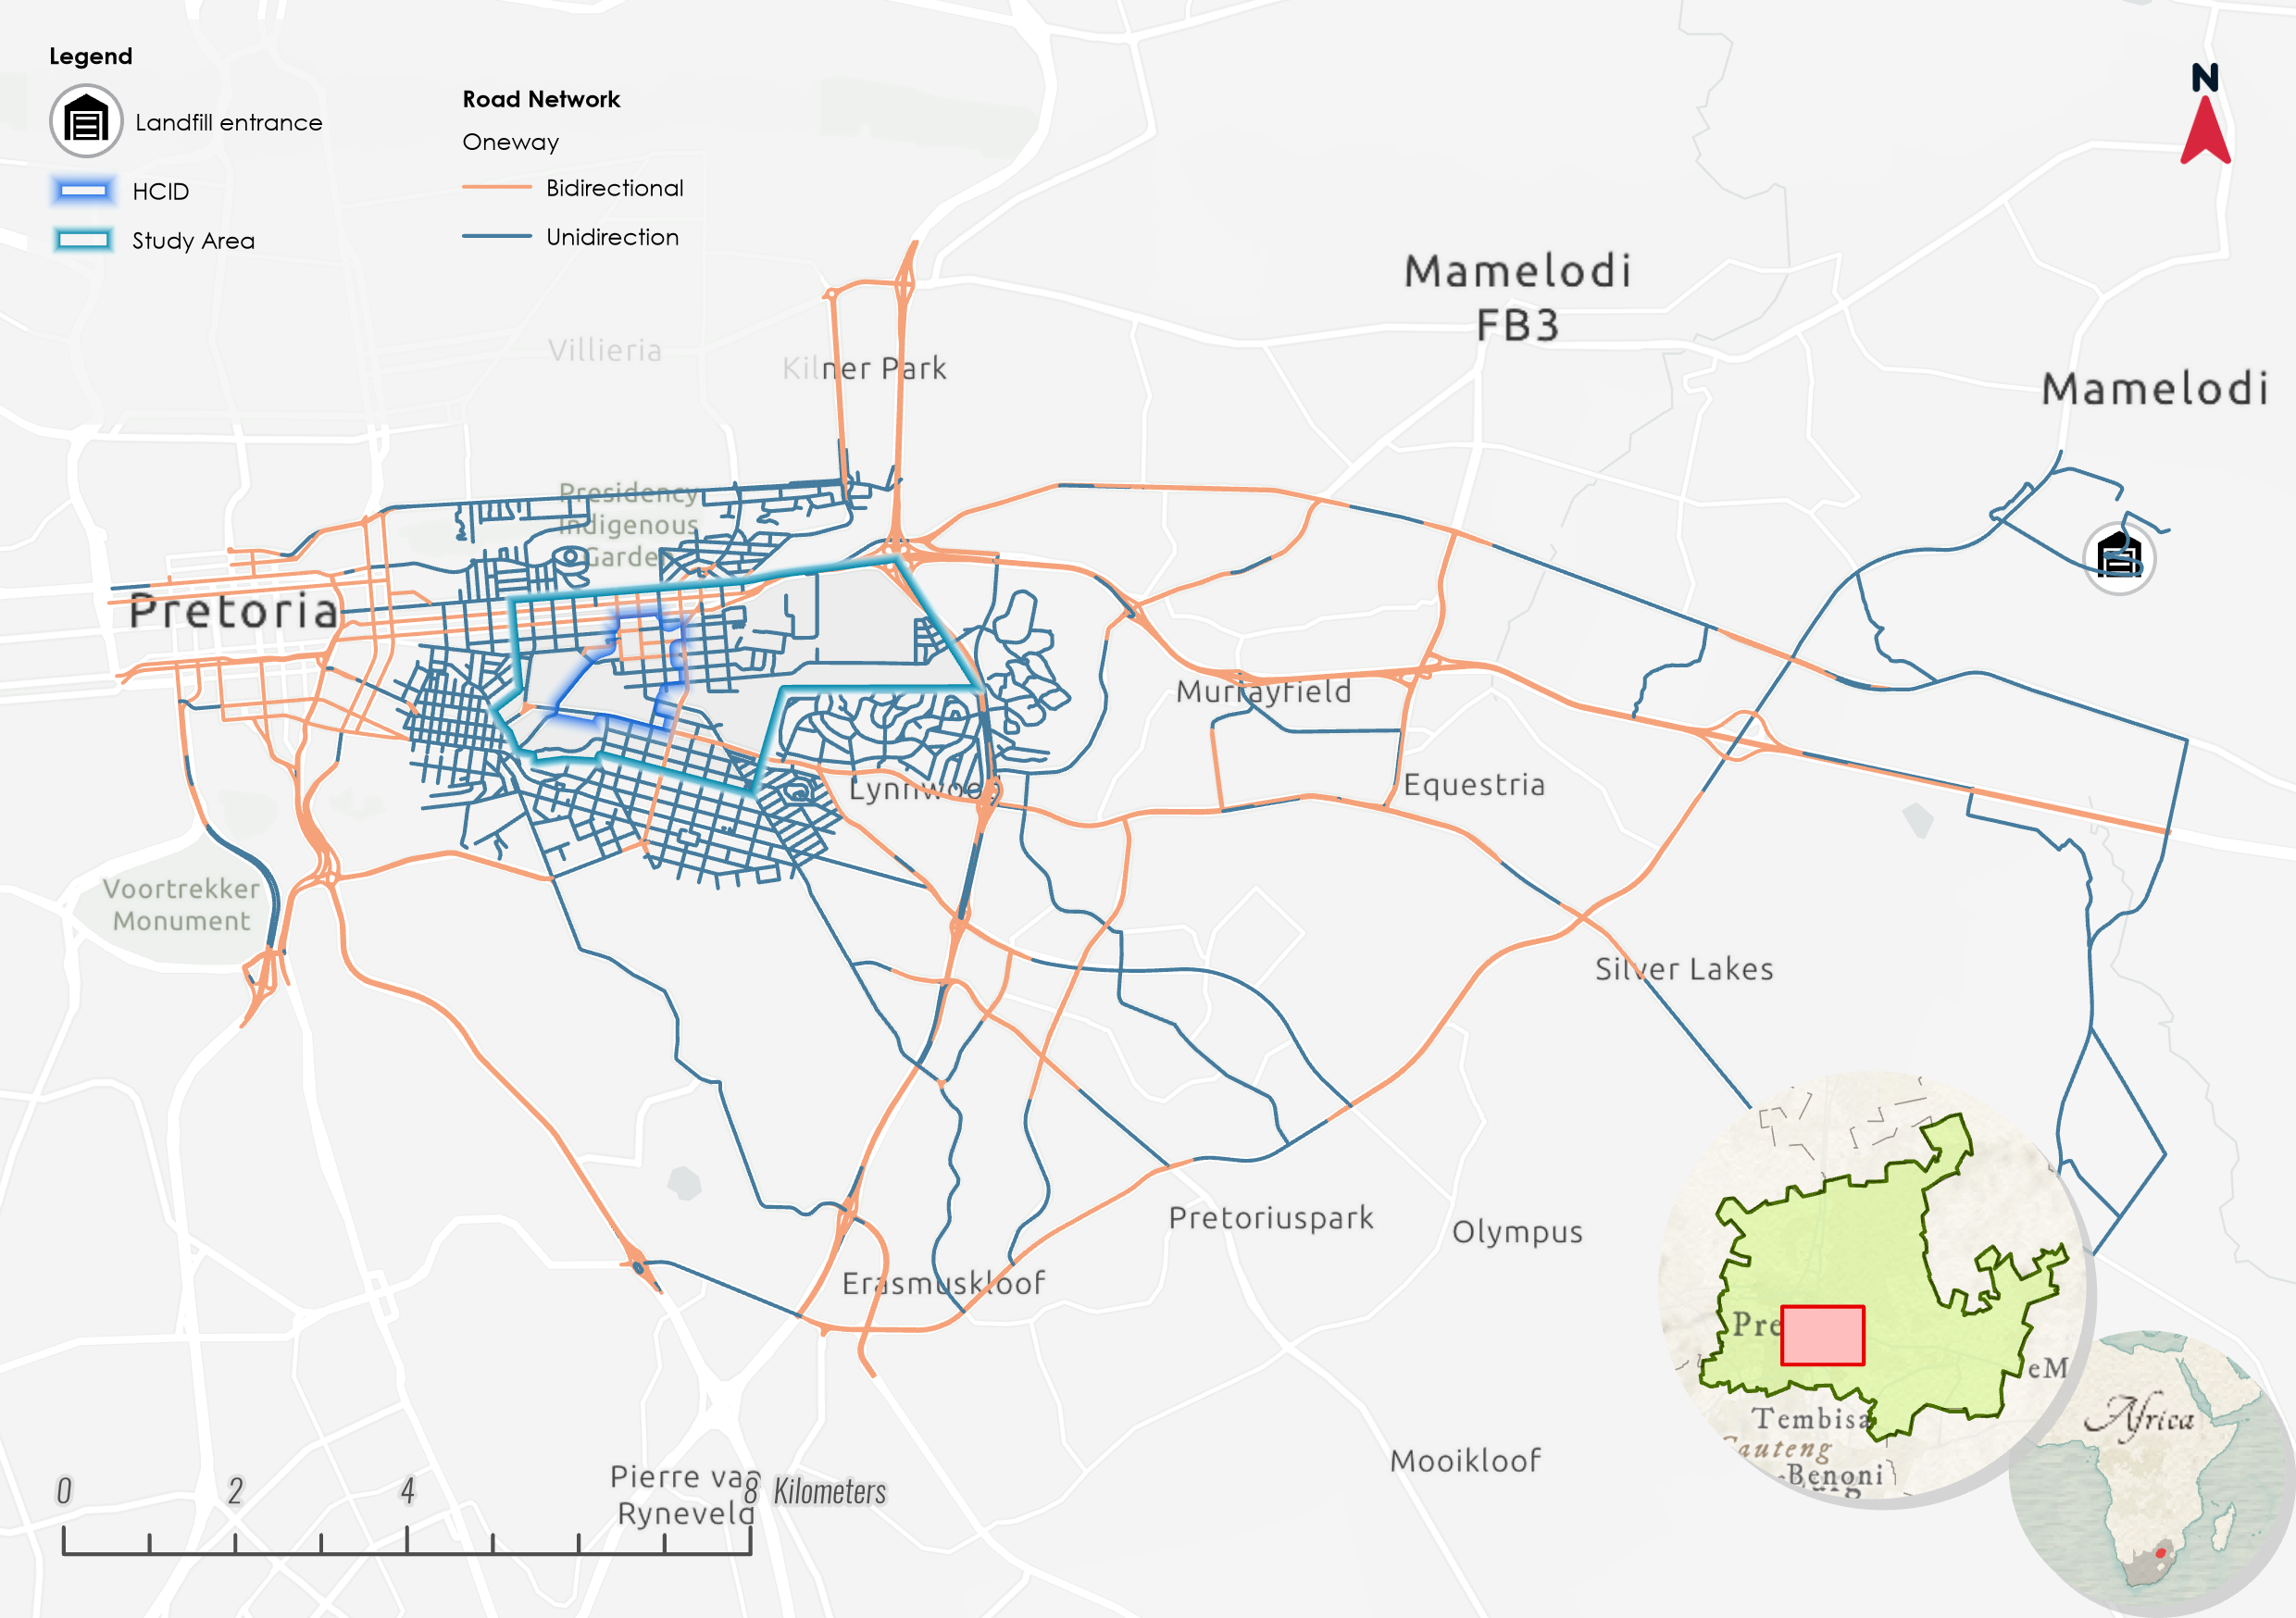
\includegraphics[width=0.85\linewidth]{Figures/Bidirectional.png}
    %     \caption{Type of Roads Map, Bidirectional or Unidirectional classification.}
    %     \label{fig:road2}
    % \end{figure*}

        %Due to the large production of the sports stadium and the fact that this building does not operate daily, it was excluded from the optimal route calculation. The absence of a designated container for this unique building and its large waste production volumes, may lead to calculation errors. Additionally, as the containers are located inside rather than in a public area, it could result in trucks focusing solely on collecting this waste, and not be representative of the normal waste collection routine in the city.%

        During waste collection simulations, a route is generated (Fig. \ref{fig:road3}) along with step-by-step navigation directions (Figure \ref{fig:road4}). After simulating several hours, the multiple paths that trucks follow each day are observed. %(Figure \ref{fig:road5}). 
        However, some locations are repeated due to constant waste overflow (Figure \ref{fig:road6}),  aligning with the results of the waste calculation.

        Each route's expected number of containers to collect varies from 112 to 213. Vehicles typically require four visits to the landfill to discharge waste and collect all containers. However, for waste generation intervals between 6 to 12 hours, nine visits to the landfill are needed. The average collection time is 5 hours and 16 minutes for a 6-hour generation period and 10 hours and 57 minutes for a 12-hour period. The average total traveled distance per route is 236.28 km, equivalent to 1,327 ZAR (69.70 USD) and 2.73 tons of CO2 emissions per route (calculated at 11.59 kg/km) \citep{EPA2023}.

    \begin{figure*}[h!]
    \centering
    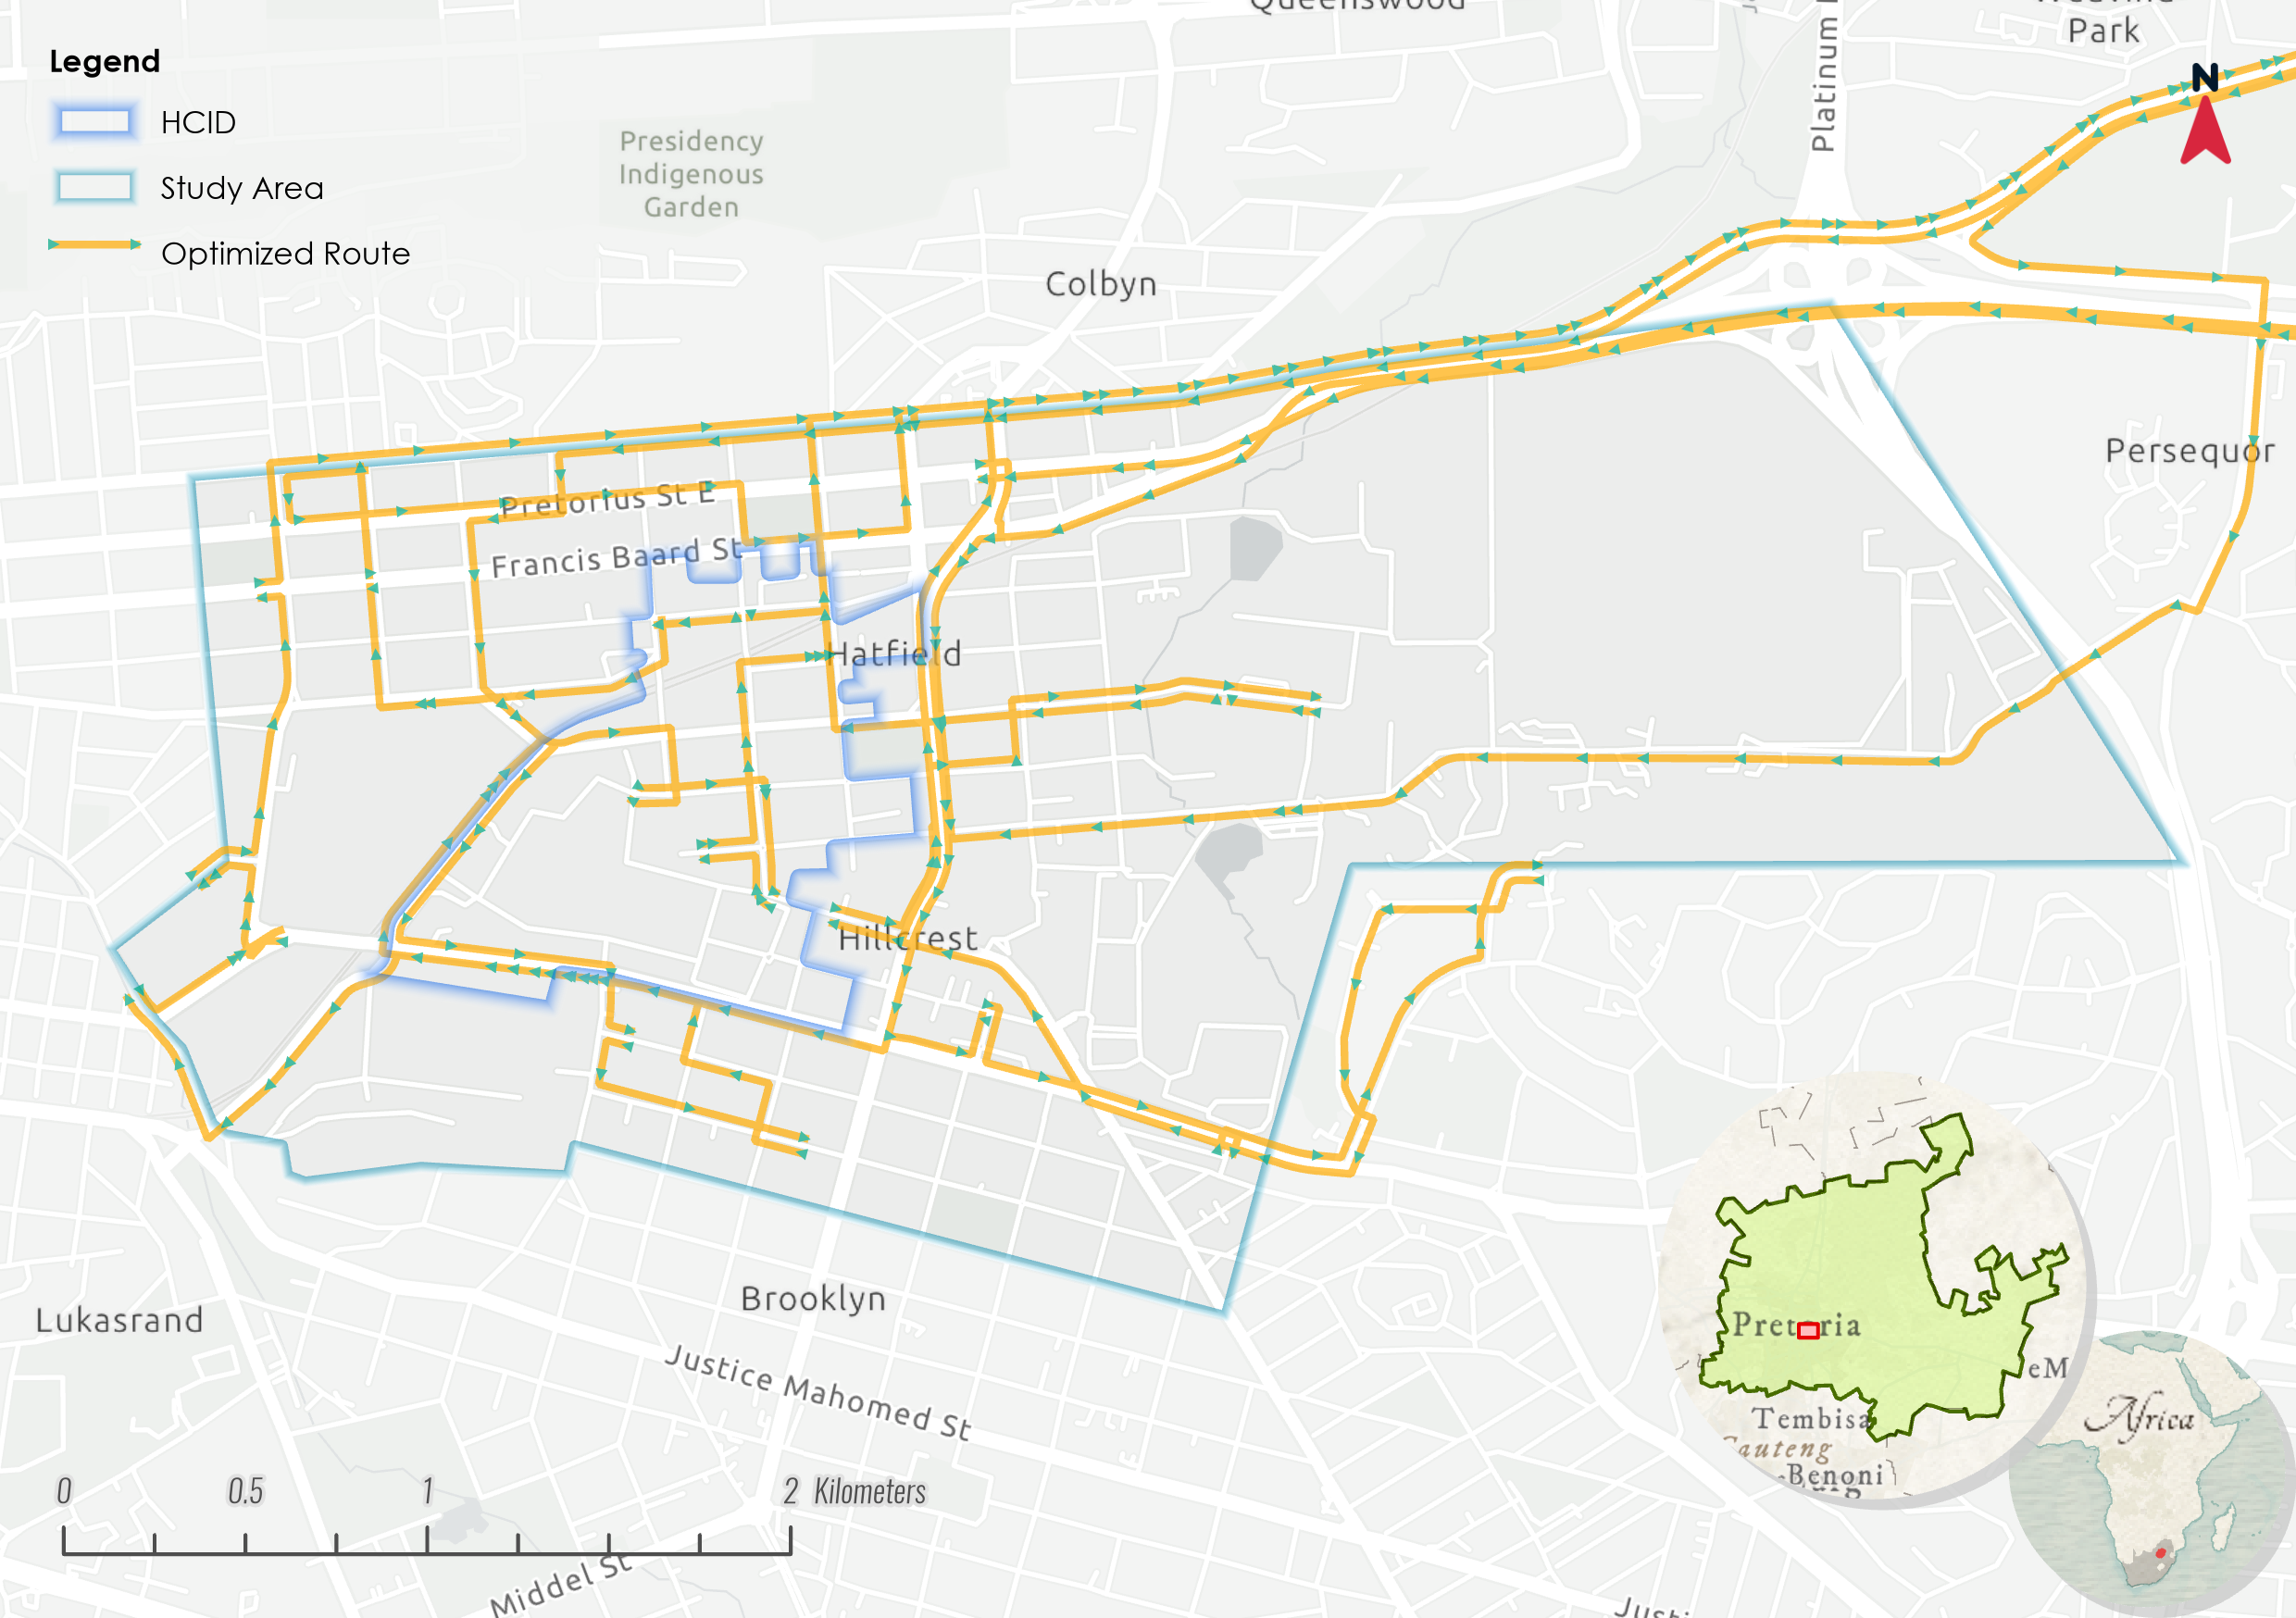
\includegraphics[width=0.8\linewidth]{Figures/Optimal route.png}
        \caption{Optimal Route Example. The route includes returns to the landfill to dump waste and restart capacity.}
        \label{fig:road3}
    \end{figure*}

    \begin{figure}[h!]
    \centering
        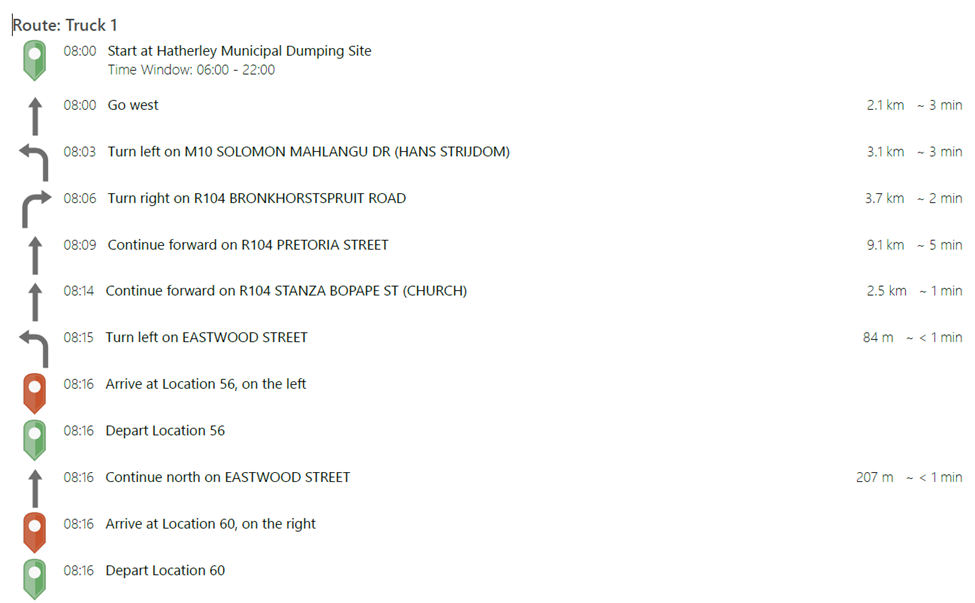
\includegraphics[width=0.9\linewidth]{Figures/road4.png}
        \caption{Step-by-step directions generated on Optimal route calculation.}
        \label{fig:road4}
    \end{figure}

    \begin{figure*}[h!]
    \centering
        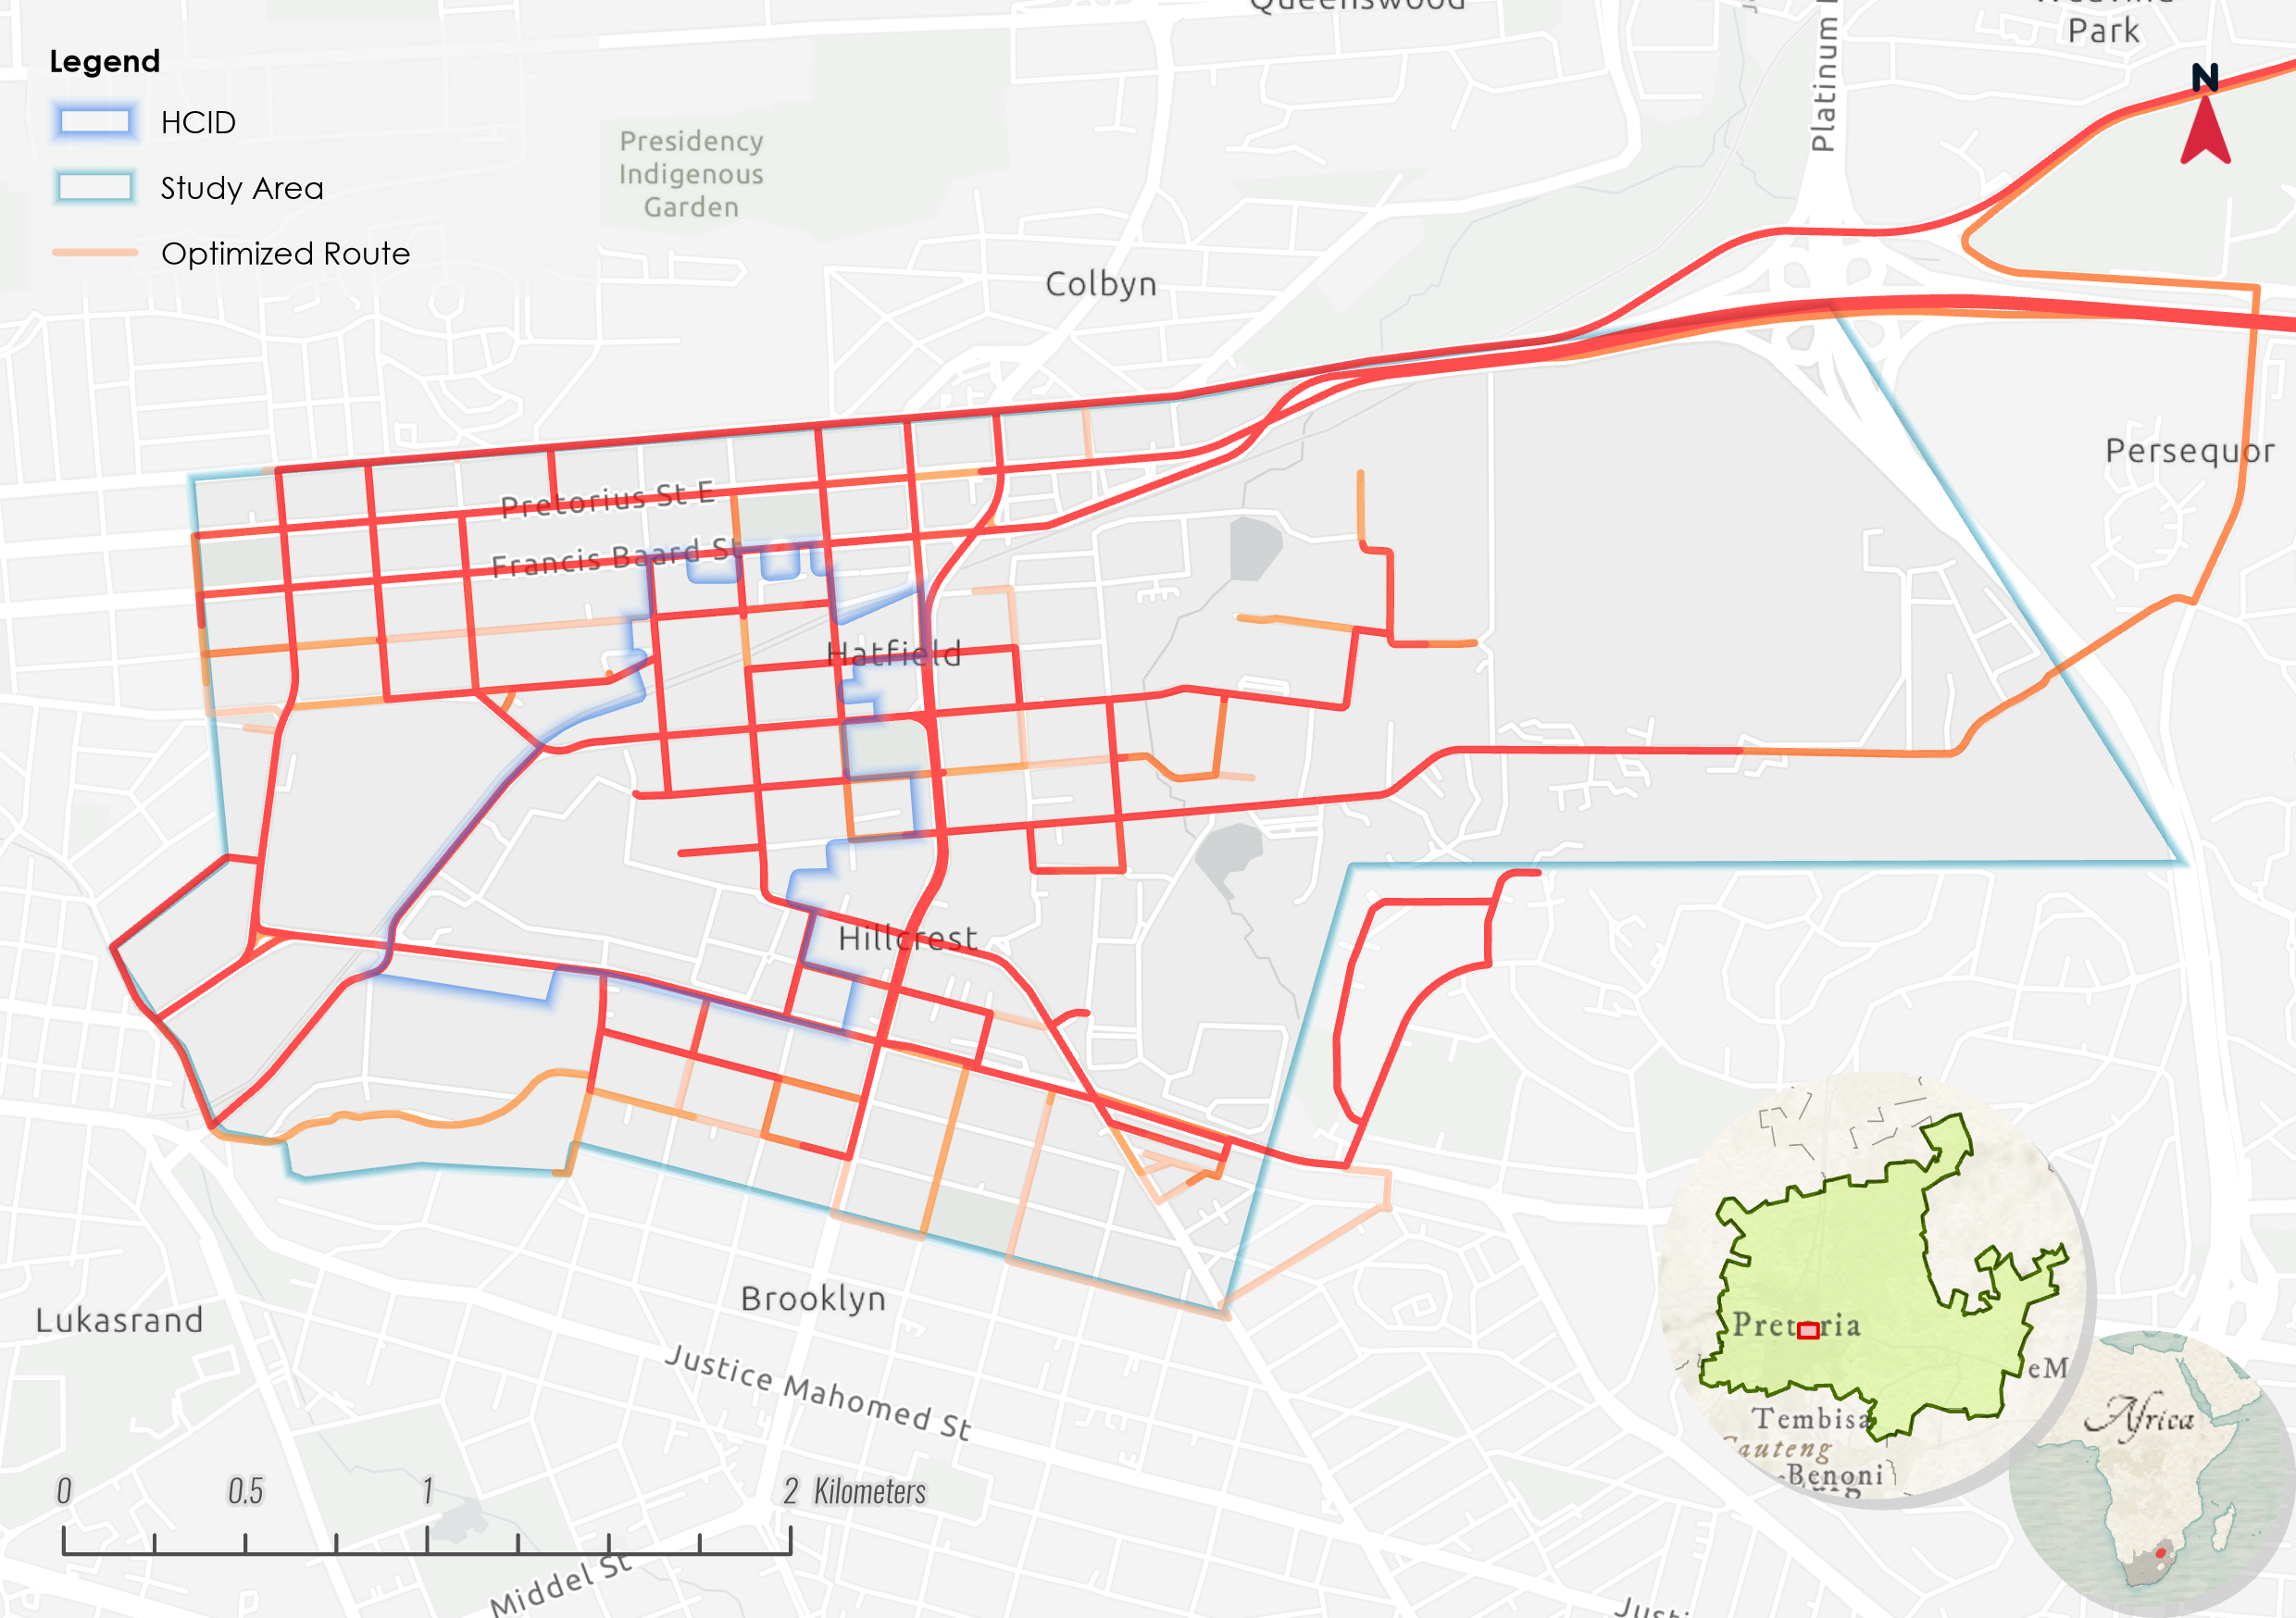
\includegraphics[width=0.8\linewidth]{Figures/Optimal Several runs.png}
        \caption{Multiple paths for waste collection. Darker colors indicate several travels on the same street segment.}
        \label{fig:road5}
    \end{figure*}

    \begin{figure*}[h!]
    \centering
        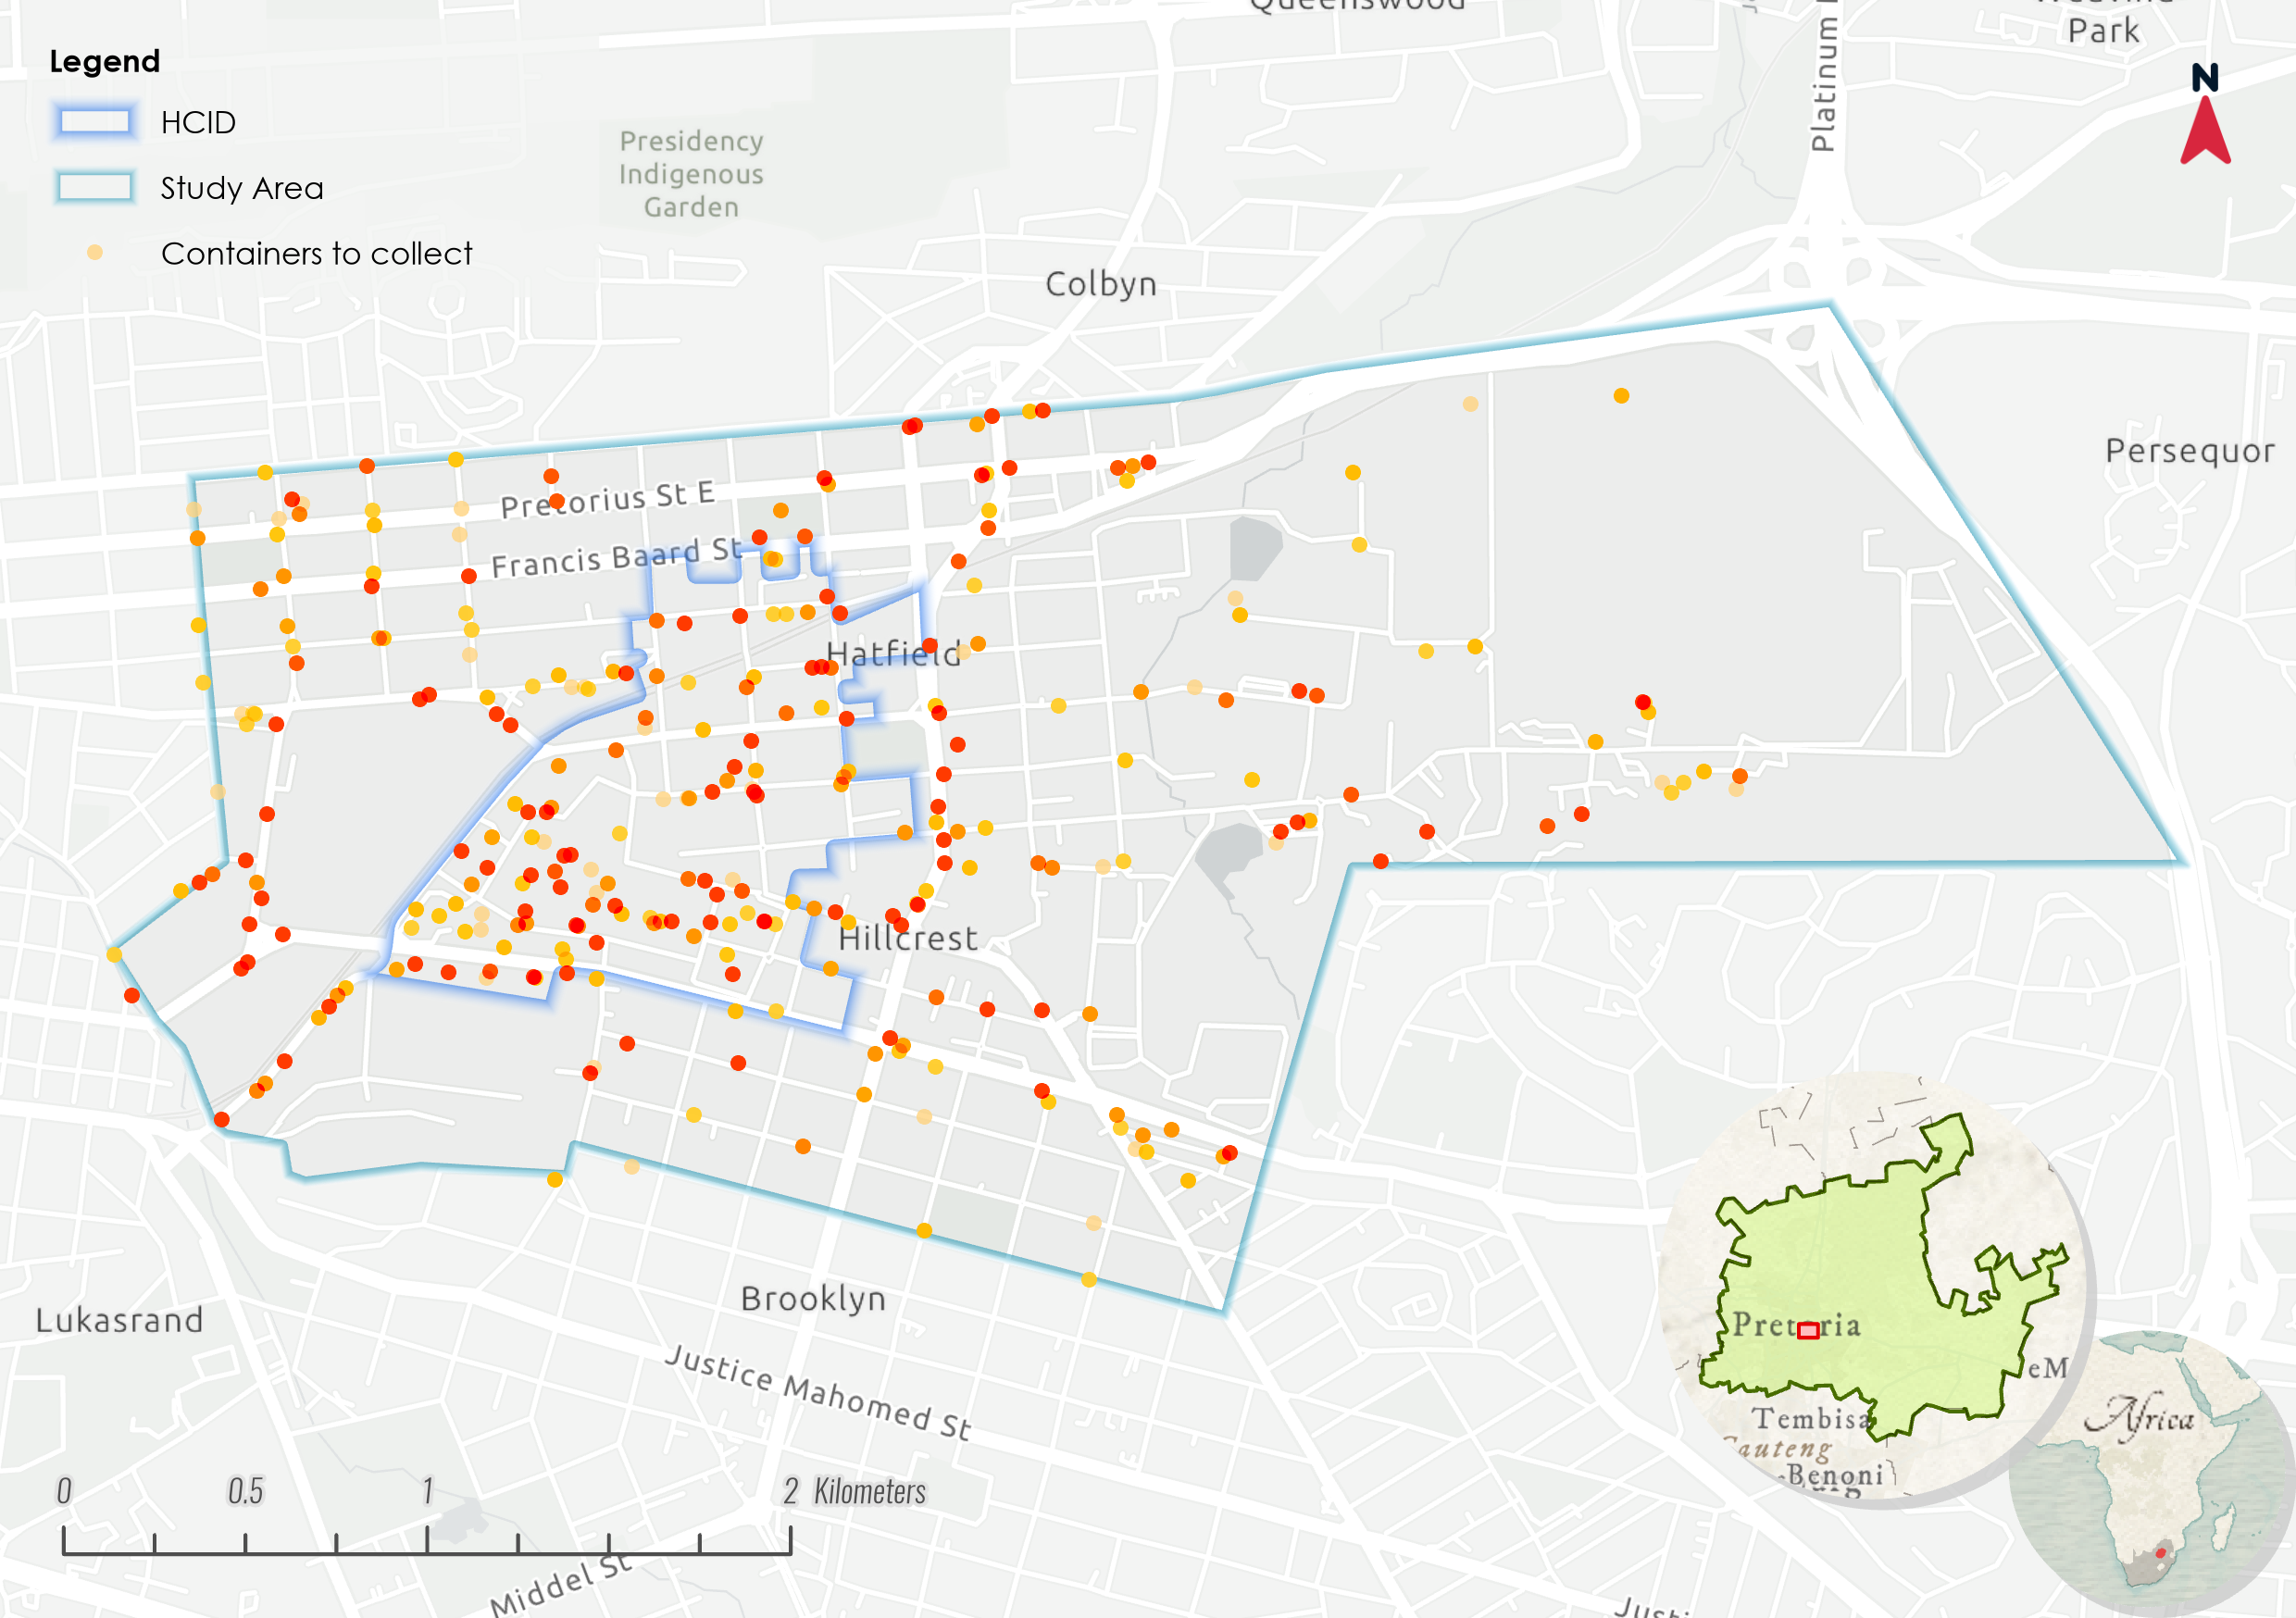
\includegraphics[width=0.8\linewidth]{Figures/Collected containers.png}
        \caption{Containers to collect. Darker colors indicate several collections required on the same container.}
        \label{fig:road6}
    \end{figure*}

    \subsection{Dashboard Design} \label{subsec:Dashboard}

    A centralized control Dashboard was designed to visualize UDT elements. It emphasizes map views of key items and indicators, interacting with the state of each map layer.  The map view includes three visualization options. The first option %(Figure \ref{fig:collections}a)
    highlights containers requiring collection on the map and displays the collection sequence along the route. This dynamic map adapts to real-time container saturation and waste accumulation values. The second option visualizes building classes and their relationship to containers, enabling users to understand the local waste distribution and travel distances to container hubs %(Figure \ref{fig:collections}b).
    The third option tracks waste littering with a heatmap of data collection reports, offering filtering options to highlight litter severity. %(Figure \ref{fig:collections}c).

    % \begin{figure*}[hp]
    % \centering
    % \begin{subfigure}[h]{0.85\linewidth}
    %     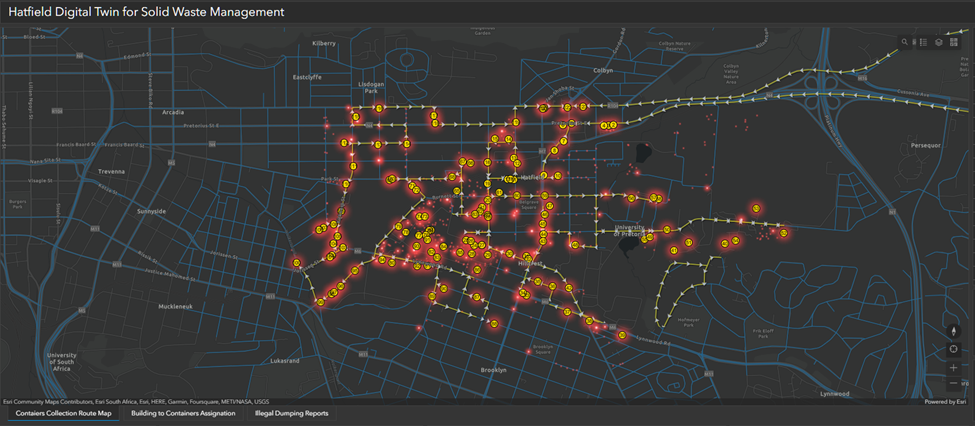
\includegraphics[width=\linewidth]{Figures/Collection1.png}
    %     \caption{Containers collection Route Map}
    %     \label{fig:collection1}
    % \end{subfigure}
    
    % \begin{subfigure}[h]{0.85\linewidth}
    %     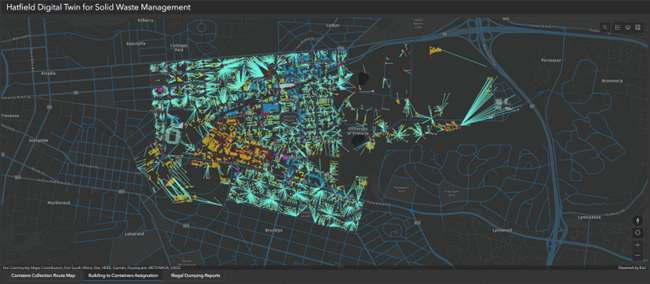
\includegraphics[width=\linewidth]{Figures/Collection2.png}
    %     \caption{Buildings to containers assignation Map}
    %     \label{fig:collection2}
    % \end{subfigure}
    % \begin{subfigure}[h]{0.85\linewidth}
    %     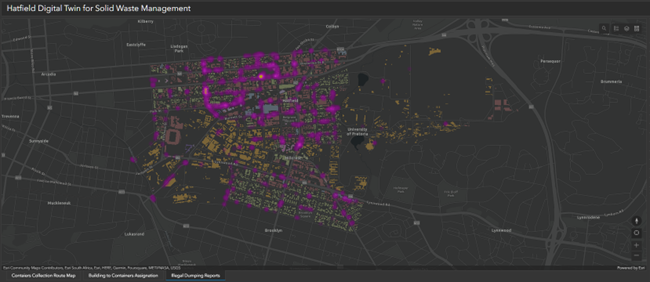
\includegraphics[width=\linewidth]{Figures/Collection3.png}
    %     \caption{Illegal Dumping Reports Map}
    %     \label{fig:collection3}
    % \end{subfigure}
    % \caption{Dashboard visualization Options}
    % \label{fig:collections}
    % \end{figure*}

    Based on identified requirements, the Dashboard displays eleven distinct indicators (Figure \ref{fig:indicators1} and Figure \ref{fig:indicators2})). The first two indicators focus on container saturation, showing average saturation and the number of containers for collection. The third indicator corresponds to map option three, displaying littering reports categorized by severity in a pie chart. The fourth indicator shows the total waste in the study area requiring collection, irrespective of container saturation. It aligns with SDG 11 monitoring (total SW production per day). Indicator 5 displays the total volume of waste production per building class, correlating with map option 2. This indicator is static as it relates to building characteristics and estimated inhabitants. Indicators 6 to 11 relate to the waste collection route and include critical planning elements such as fuel cost, CO2 emissions, total traveled distance, total operation time, number of required returns to landfill (after the truck's capacity is full), and a sequence list for container collection. This sequence is interactive, with activation highlighting items in map option 1.

    \begin{figure}[h!]
    \centering
        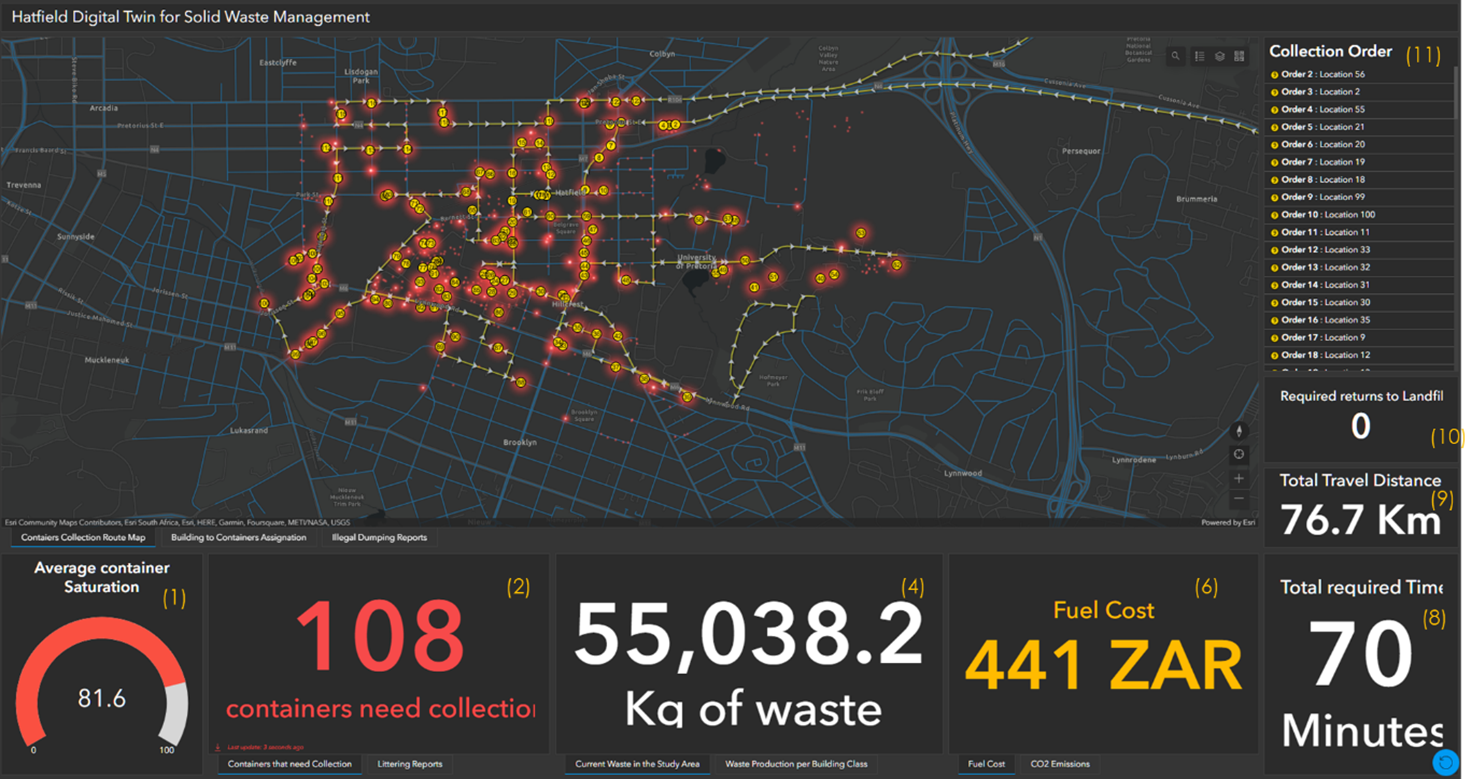
\includegraphics[width=0.9\linewidth]{Figures/indicators1.png}
        \caption{Dashboard and indicators (signaled on yellow brackets)}
        \label{fig:indicators1}
    \end{figure}

    \begin{figure}[h!]
    \centering
        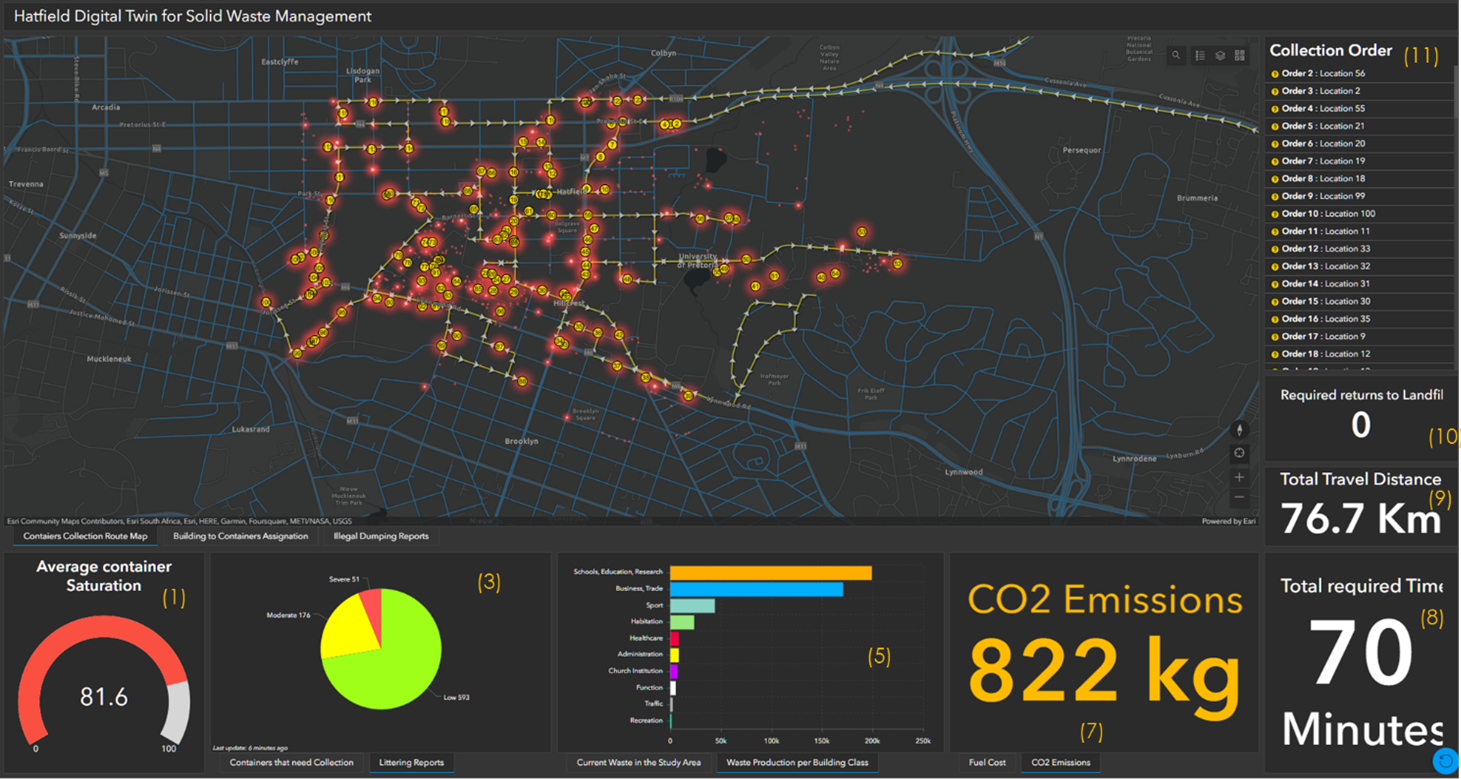
\includegraphics[width=0.9\linewidth]{Figures/indicators2.png}
        \caption{Dashboard and indicators (signaled on yellow brackets)}
        \label{fig:indicators2}
    \end{figure}

    \subsection{Waste Digital Twin Assessment} \label{subsec:Assessment}
   The simulation speed varies between local and cloud-run services. In the local setup, each hour of waste generation calculation takes an average of 5.02 seconds, while calculating optimal collection routes takes 2.72 minutes. Conversely, on the Cloud service , each simulated hour takes 4.18 minutes (a 4,996\% increase), and the optimal route calculation extends to 4.93 minutes (a 181\% increase). This is attributed to the process structure, wherein online stored layers require downloading records, performing individual record updates, and immediately updating tuples to the layer instead of updating all tuples at once at the end of each run.

    The stakeholder assessment survey response rate was 38.1\% (8/21), with one respondent unable to access the Dashboard, and their response was excluded from the analysis. Overall, the Dashboard obtained high scores, with only the Data Accuracy and Decision-making Support indicator scoring below 4 points. A third of the respondents (28.57\%) do not consider that the Dashboard efficiently conveys the container waste quantity and waste generation per building, nor does it accurately consider container saturation. Therefore, improvement and simplification are necessary to enhance the communicative value of the Dashboard, for example, including waste status per container and building-to-container waste generation. Conversely,  85.71\% of respondents rate the Dashboard with 5 points, which indicates that it provides valuable information for collaboration to address collective waste management challenges. (See Table \ref{tab:stakeAssesment} for indicator scores and category averages).

    \begin{table*}[h!]
        \caption{Dashboard survey Score based on a 5-point Likert scale.}
        \label{tab:stakeAssesment}
        \scriptsize
        \begin{tabularx}{\linewidth}{l LLL}
            \toprule
            Category & Indicator                                  & Score & Category Score \\ \midrule
            \multirow{2}{*}{\shortstack{User Friendliness \\and Interactivity}}              & Ease of Use                               & 4.48 & \multirow{2}{*}{4.27} \\
                    & Data Exploration                           & 4.05  &                \\
            \multirow{2}{*}{Spatial Interface}                                & Map Visualization                         & 4.53 & \multirow{2}{*}{4.43} \\
                    & Ease of Learning                           & 4.33  &                \\
            \multirow{2}{*}{\shortstack{Consensus, Effectiveness \\ and Communicative value}} & Data Accuracy and Decision-making support & 3.93 & \multirow{2}{*}{4.11} \\
                    & Stakeholder Communication and collaboration & 4.29  &                \\ \bottomrule
        \end{tabularx}
    \end{table*}

    Due to the low response, open conversation was encouraged to further garner insights about the tools' usefulness and communicative value. The conversation highlighted a lack of clarity in explaining the support system provided by the UDT, and the tool explanation was not assertive enough. This indicates insufficient engagement and explanation of the tool's purpose and goals, hindering stakeholders' understanding and adoption of the tool's capabilities.

    Alternatively, a stakeholder acknowledged that the Digital Twin can demonstrate the added value of their work in public spaces by visualizing their impact on SW management within their operational area. They appreciated the heatmaps as a positive feature for displaying the operational benefits of additional waste collection, distinct from those provided by the municipality. A participant noted a limitation of the routing approach, excluding restricted areas, roads within private property, or containers in restricted access areas. Due to the lack of available data and access restrictions, the model could not consider these factors, highlighting the need for improvement in future iterations. Participants appreciated the data accessibility and user-friendly information provided despite not having expertise in geo-spatial software. They highlight the importance of making the information accessible to more people (for example, students or research groups). However, they emphasize the need for incentives to encourage citizen engagement in self-reporting or data contribution to the project. Regarding design preferences, participants suggest alternative color options for the Dashboard to improve readability.

    \section{Discussion} \label{sec:Discussion}

    The discussion is divided into three parts: 1) evaluating the prototype based on the Gemini Principles, 2) discussing its benefits and practical implications, and 3) addressing considerations such as security, data accuracy, scalability, stakeholder engagement, and challenges encountered. This section shows the importance of UDTs in urban waste management and their potential for promoting sustainability and cost-effectiveness.

    
    \subsection{Findings}\label{subsec:Findings}
    Identifying and classifying the stakeholders in developing digital twins is sometimes overlooked by other researchers \citep{Bartos2021, Jiang2022, Xu2022, Yu2023}. Analyzing stakeholders based on the adapted salience model identified crucial end-users of the tool: the City Improvement District, the Ward representatives, and the Municipality Waste Department. These stakeholders, with shared political power dynamics, emerge as key users due to their influential roles and relationships within the stakeholder network.

    Using the adapted salience model in this way, combined with pairwise comparison, helps mitigate the subjectivity inherent in classifying stakeholders into different typologies, as outlined by \citet{Mitchell1997} and \citet{Shafique2022}. Indeed, while the adapted salience model with pairwise comparison reduces subjectivity, it does not eliminate it entirely, as there is still a degree of subjectivity involved in analyzing and comparing stakeholders within their categories. However, this method provides a structured approach to determine the importance of each stakeholder, taking into account specific cases and locations. In this case, although the Ward Councilor was not actively involved in the UDT piloting process, other stakeholders identified them as an essential agent. The Ward Councilor plays a crucial role in facilitating communication between residents and other actors in the locality. This situation may not hold true in other regions of the country or context. The developing world regions have a wide range of urban contexts and structures. Using the adapted salient model combined with a process of co-creation with local stakeholders exposes these hyper-local nuances for relevant UDTs. For instance, smaller cities and rural areas may exhibit different dynamics, where social leaders and direct resident-to-municipality contact play a more prominent role compared to highly urbanized areas with stronger and structured political relationships.

SW container spatial distribution was found despaired across the study area, with some areas experiencing overflow and environmental risks due to an excess of waste, while others suffer from littering and illegal dumping due to insufficient containers. Specifically, the data highlighted the CID's efforts in litter cleanup and the concentration of containers near educational facilities. These insights suggest targeted and practical interventions, such as installing larger containers near the stadium and shopping centers, increasing collection frequency along the major traffic route, implementing traffic restrictions, or enhancing road maintenance along frequently traversed routes by collection trucks. Additionally, areas with lower waste generation, particularly residential zones, could benefit from centralized neighborhood waste collection points rather than in their own front yards. Importantly, this collaborative data-sharing initiative provided stakeholders with a unified understanding of the city's waste landscape, contrasting with previously fragmented perspectives and isolated agendas by individual stakeholders.
    
Geospatial data integration allowed to estimate population and building use aiming to generate Waste generation simulations. This offers insights into waste flows from buildings to containers, highlighting areas with high production and limited capacity requiring intervention. While the building-to-container assignment may lack accuracy due to access restrictions, it serves as a proxy for collection points, aiding in the strategic placement of larger containers to optimize truck loading times, which are currently going home by home. Clustering can further reduce operational costs by minimizing travel time and workforce hours. However, it is crucial to conduct waste flow analysis using Manhattan distance movement, considering the constraints of city navigation rather than relying on Euclidean distances.

    The proposed container aggregation method is simpler compared to other authors such as \citet{al-refaieOptimizationModelsClustering2020} and \citet{viktorinHierarchicalClusteringbasedAlgorithms2023}, as it involves fewer elements for analysis. As the scale of the problem increases with more buildings and containers, the overall performance may decrease. However, since only the number of inputs affects performance, the method can quickly adapt to larger data sets and changing volumes as the city integrates this technology and citizens provide new reports.

    The current weekly waste collection scheme using a single vehicle appears to be inadequate for significant waste production in this context. However, with multiple waste collection companies serving businesses and large producers, it's crucial to map all collection actors, daily generated quantities, and the rate of waste segregation at the source. This comprehensive understanding of waste flows is essential for recalculating optimal collection routes.

    The proposed waste collection optimization aims to consolidate the collection of multiple nodes, thereby reducing operational times, fuel consumption, and resulting greenhouse gas emissions. The optimized collection routes would cost 1,932,554 ZAR (101,623 USD) annually in the study area alone, representing 0.11\% of the overall city Waste Management budget \citep{tshwane20232024MediumtermRevenue2023}. This amount is significant considering the study area covers only 0.15\% of the city, and the cost is solely related to fuel consumption. 
    Additional costs related to waste management, including landfill operation, workers' wages, provision of containers and trash bags, and vehicle maintenance, need to be considered. While this scenario reflects an optimized waste collection routing, the lack of data on current vehicle paths, total fuel consumption, and detailed collection and transport expenditure makes it impossible to estimate the improvement rate. However, this cost estimation emphasizes expanding the total budget to ensure the city can cover all SW management costs.
    
    The limited number of responses for this pilot makes it difficult to conclusively determine if an operational control dashboard is the most effective method for integrating and making information accessible to stakeholders in the SW management twinning workflow. While stakeholders provided high scores in various indicators such as user-friendliness, interactivity, spatial interface, consensus, effectiveness, and communicative value, more respondents would be needed to draw definitive conclusions.

     Despite the technical challenges involved in creating the UDT and its outcomes, such as tracking appropriate performance metrics or revealing socio-political shortcomings, the greatest value of this bottom-up people-first process lies in its ability to identify holistic areas for waste improvement in cities. By taking a holistic approach, the UDT reveals numerous non-technical possibilities that could be addressed through urban strategic events involving multiple stakeholders. In this way, the Waste UDT serves as a means to an end in serving the greater good rather than merely functioning as a technical instrument of urban management.

\subsection{Gemini Principles analysis} \label{subsec:Gemini}
    This solid waste UDT prototype offers numerous benefits, including targeted waste collection efforts to reduce unnecessary trips and time savings. It identifies littering hotspots, enabling strategic measures like increasing bin numbers or awareness campaigns. Optimizing collection routes and schedules enhances efficiency and reduces fuel consumption, labor, maintenance, and greenhouse gas emissions. Proper waste management promotes a clean, hygienic environment, aligning with Sustainable Development Goals 11 and 12. It also contributes to aesthetically pleasing surroundings, improving residents' and visitors' overall quality of life. The UDT provides valuable waste generation patterns, bin usage, and littering data, enabling appropriate data-driven decision-making and evidence-based policies. Resident participation in reporting waste disposal and collection patterns enhances waste governance.
    
    %Although the purpose of digital twinning for waste management is evident for these authors, it is necessary to include better communication practices to allow stakeholders to understand the capabilities and potential uses of this approach. During the stakeholders’ workshop, it was clear that the purposefulness is unclear for all stakeholders.%

    Data collection is open to all participants, but accuracy procedures must be integrated for quality assurance. Epicollect5 presents a challenge in moderating photographs to prevent offensive or harmful content. Implementing a robust content moderation system with algorithms and human oversight is necessary to maintain UDT integrity and ensure a positive user experience.
 
    Data accuracy, especially the number of residents per building, is constrained by the method used by \citet{Schiavina2022}, leading to unrealistic imbalances like single houses with 16 inhabitants. Integrating census data, such as the recently published results of Census 2022 from the Department of Statistics South Africa, could enhance accuracy \citep{statisticssouthafricaCensus202223}.

    The architecture in Figure \ref{fig:architecture} supports scalability for increasing container numbers, volume capacity, and waste generation, as well as expanding the road network for wider coverage. It also accommodates different types of collection vehicles.  Encouraging more user feedback and co-creative stakeholder engagement ensures relevant adaptation to evolving needs and technological advancements, making this UDT prototype a sustainable tool for long-term waste management solutions.

    \subsection{Limitations} \label{subsec:limitations}

    The waste calculations and categorization of non-residential buildings were based on data from Athens, Greece in 2008, a non-African country with a GDP per capita more than double that of South Africa  \citep{Bank2021}. The significant differences in time (15 years ago), consumption patterns, type of business, and waste segregation can greatly impact the amount of waste generated at each building. Therefore, the waste generation calculations may not accurately reflect the context of the City of Tshwane.

    Comparing the generated waste data to the real scenario was challenging due to the lack of existing data on landfill volumes. Landfill operators do not register the dumped volume, operating more as open-access dumpsters than regulated landfills. Limited research resources constrained the integration and availability of the dashboard online. Establishing a mature open-source UDT accessible via HTTP protocols would entail acquiring a cloud server virtual machine and installing various packages and libraries. Financial costs for deployment, operation, and maintenance were not covered in this research. Additionally, developing a waste management UDT on open-source platforms necessitates a transdisciplinary team with expertise in environmental management, finance, computer science, advanced programming, urban strategy, local social dynamics, and geographical information systems. This diverse team with unique skill sets is essential for delivering value to all local stakeholders.

    \section{Conclusions} \label{sec:conclusions}

    Digital twinning serves as the foundation for a decision support system in strategic waste management initiatives. When evaluating the necessity for new or modified waste containers, UDTs offer realistic simulations to assess their impact on collection efficiency and cost-effectiveness. Visualizing this data allows waste management authorities to pinpoint areas with insufficient coverage and strategically plan container placement for enhanced waste collection in dynamic and tactical ways. Moreover, UDTs facilitate adaptation to evolving waste disposal needs by providing a dynamic model continuously updated with real-world data.
    
    Involving citizen participation in the proposed method mitigates challenges identified in Artificial Intelligence computer vision detection research, such as location accuracy, high resource requirements, and labeling disagreements. It underscores the significance of citizen testimony in mapping solid waste and fosters awareness and sensitivity to waste management among the public. Real-time monitoring helps address the randomness of low-severity littering, contributing to improved solid waste management involving multiple stakeholders.  The design of this UDT facilitates collaborations between stakeholders, enhancing communication and transparency in decision-making processes involving diverse stakeholders. By applying these technologies, the connection between urban developers, urban managers, and citizens can be strengthened, enabling residents to participate in the governance of local solid waste management.
    
    The UDT design facilitates various tests and calculations, enabling the detection of areas where overflow may occur by comparing current container volume capacity with waste generation.  By modifying input values, such as changes in population or consumption habits, it's possible to calculate the relevant capacity for specific locations and simulate the potential effects on waste collection across a city.

    Waste collection often accounts for a significant portion of a city's budget. By implementing a digital twinning approach to urban waste management systems, authorities and citizens can access real-time information on waste container fill levels and plan optimized collection routes. On the city management side, this can reduce fuel consumption, lower vehicle emissions, and minimize operational expenses, resulting in a more sustainable and cost-effective waste management process. There's potential for incentives like dynamic tax breaks or property levies for residents generating less waste or specific types of waste. This could reduce the existing strain on landfills, improve urban circularity objectives, improve public awareness, and align with several related SDG objectives.

    %\textit{Crucial} and \textit{Definitive} stakeholders can gain insights into the system's dynamics by visually representing the city's waste management infrastructure, including containers, littering, collection vehicles, and disposal facilities. This allows them to simulate different scenarios and optimize collection strategies based on various factors, such as waste generation patterns, changes in population, and traffic restrictions.%

     By developing and co-creating holistic digital counterparts of urban waste management infrastructure and processes, policymakers, stakeholders, and residents can comprehensively understand the current state of the urban solid waste landscape. This collective knowledge serves as a holistic decision-making support system for practical, targeted, and dynamic interventions relevant to the activities of the city over time. Through collective efforts and integration of technology and community engagement, improved solid waste management can be achieved, even in resource-constrained settings such as South Africa. UDTs go beyond being digital products; they serve as catalysts for collective urban processes that contribute to the greater good.

    %\printcredits

    \bibliographystyle{apalike-ejor} 
    \bibliography{Main.bib}
    \appendix \label{appendix}
    \end{document}
    \endinput
